\pdfoutput=1
\pdfcompresslevel=9
\pdfinfo
{
    /Author (Krzysztof Opasiak)
    /Title (Rozproszony monitoring systemów komputerowych)
    /Subject (Tematyka)
    /Keywords (Slowa kluczowe)
}
%\documentclass[a4paper,polish,onecolumn,oneside,floatssmall,11pt,titleauthor,wide,openright]{mwrep}
%\usepackage[scale={0.7,0.8},paper=a4paper,twoside]{geometry}
\documentclass[a4paper,onecolumn,oneside,11pt,wide,floatssmall]{mwrep}
% \usepackage{polish}
\usepackage{amsmath}
\usepackage{amsfonts}
\usepackage{amssymb}
\usepackage{amsthm}
\usepackage{bookman}
\usepackage{longtable}
\usepackage{listings}
\usepackage{url}
\usepackage{geometry}
\usepackage[utf8x]{inputenc}
\usepackage[T1]{fontenc}
% \usepackage{t1enc}
% \usepackage[pdftex, bookmarks]{hyperref}
\usepackage[pdftex, bookmarks=false]{hyperref}
\def\url#1{{ \tt #1}}

\usepackage{listings}
\usepackage{float}
\restylefloat{table}

% marginesy
\textwidth\paperwidth
\advance\textwidth -55mm
\oddsidemargin-0.9in
\advance\oddsidemargin 33mm
\evensidemargin-0.9in
\advance\evensidemargin 33mm
\topmargin -1in
\advance\topmargin 25mm
\setlength\textheight{48\baselineskip}
\addtolength\textheight{\topskip}
\marginparwidth15mm

\clubpenalty=10000 % to kara za sierotki
\widowpenalty=10000 % nie pozostawia wdów
\brokenpenalty=10000 % nie dzieli wyrazów pomiędzy stronami
\sloppy

\tolerance4500
\pretolerance250
\hfuzz=1.5pt
\hbadness1450

% ŻYWA PAGINA
\renewcommand{\chaptermark}[1]{\markboth{\scshape\small\bfseries \
#1}{\small\bfseries \ #1}}
\renewcommand{\sectionmark}[1]{\markboth{\scshape\small\bfseries\thesection.\
#1}{\small\bfseries\thesection.\ #1}}
\newcommand{\headrulewidth}{0.5pt}
\newcommand{\footrulewidth}{0.pt}
\pagestyle{uheadings}

\usepackage[pdftex]{color,graphicx}
\usepackage{epstopdf}
\usepackage[polish]{babel}

% \textheight232mm
% \setlength{\textwidth}{\textwidth}
% \setlength{\oddsidemargin}{\evensidemargin}
% \setlength{\evensidemargin}{0.3cm}
\usepackage[sort, compress]{cite}

%\usepackage{multibib}
%\newcites{bk,st,doc,web}{Książki i~artykuły,Standardy i~zalecenia,Dokumentacja produktów,Publikacje i~serwisy internetowe}

\theoremstyle{definition}
\newtheorem{defn}{Definicja}[section]
\newtheorem{conj}{Teza}[section]
\newtheorem{conjmain}{Teza}
\newtheorem{exmp}{Przykład}[section]

\theoremstyle{plain}% default
\newtheorem{thm}{Twierdzenie}[section]
\newtheorem{lem}[thm]{Lemat}
\newtheorem{prop}[thm]{Hipoteza}
\newtheorem*{cor}{Wniosek}

\theoremstyle{remark}
\newtheorem*{rem}{Uwaga}
\newtheorem*{note}{Uwaga}
\newtheorem{case}{Przypadek}

\definecolor{ListingBackground}{rgb}{0.95,0.95,0.95}

\begin{document}

% kody źródłowe wplatane w tekst
\lstdefinestyle{incode}
{
basicstyle={\footnotesize},
keywordstyle={\bf\footnotesize\color{blue}},
commentstyle={\em\footnotesize\color{magenta}},
numbers=left,
stepnumber=5,
firstnumber=1,
numberfirstline=true,
numberblanklines=true,
numberstyle={\sf\tiny},
numbersep=10pt,
tabsize=2,
xleftmargin=17pt,
framexleftmargin=3pt,
framexbottommargin=2pt,
framextopmargin=2pt,
framexrightmargin=0pt,
showstringspaces=true,
backgroundcolor={\color{ListingBackground}},
extendedchars=true,
% title=\lstname,
captionpos=b,
% abovecaptionskip=1pt,
% belowcaptionskip=1pt,
frame=tb,
framerule=0pt,
}

% kody źródłowe z podpisem
\lstdefinestyle{outcode}
{
basicstyle={\footnotesize},
keywordstyle={\bf\footnotesize\color{blue}},
commentstyle={\em\footnotesize\color{magenta}},
numbers=left,
stepnumber=5,
firstnumber=1,
numberfirstline=true,
numberblanklines=true,
numberstyle={\sf\tiny},
numbersep=10pt,
tabsize=2,
xleftmargin=17pt,
framexleftmargin=3pt,
framexbottommargin=2pt,
framextopmargin=2pt,
framexrightmargin=0pt,
showstringspaces=true,
backgroundcolor={\color{ListingBackground}},
extendedchars=true,
% title=\lstname,
captionpos=b,
% abovecaptionskip=1pt,
% belowcaptionskip=1pt,
frame=tb,
framerule=0.1pt,
}

\renewcommand*\lstlistingname{Wydruk}
\renewcommand*\lstlistlistingname{Spis wydruków}

\pagenumbering{roman}
\renewcommand{\baselinestretch}{1.0}
\raggedbottom

\begin{titlepage}
    % Strona tytułowa
    \vbox to\textheight{\hyphenpenalty=10000
    \begin{center}
	\begin{tabular}{p{107mm} p{9cm}}
	    \begin{minipage}{9cm}
	      \begin{center}
	      Politechnika Warszawska \\
	      Wydział Elektroniki i~Technik Informacyjnych \\
	      Instytut Informatyki
	      \end{center}
	    \end{minipage}
	    &
	    \begin{minipage}{8cm}
	    \begin{flushleft}
	     \footnotesize
	      Rok akademicki 2013/2014
	    \vspace*{2.75\baselineskip}
	    \end{flushleft}
	    \end{minipage} \\
	\end{tabular}
        \vspace*{2.5\baselineskip}
	\par\vspace{\smallskipamount}
	\begin{center}
		
\includegraphics[angle=0,scale=1]{img/logo_pw.png}
	\end{center}
	\vspace*{2\baselineskip}{\LARGE Praca dyplomowa inżynierska\par}
	\vspace{3\baselineskip}{\LARGE\strut Krzysztof Opasiak\par}
	\vspace*{2\baselineskip}{\huge\bfseries Rozproszony monitoring systemów komputerowych\par}

	\vspace*{7\baselineskip}
	\hfill\mbox{}\par\vspace*{\baselineskip}\noindent
	\begin{tabular}[b]{@{}p{3cm}@{\ }l@{}}
	    {\large\hfill } & {\large }
	\end{tabular}
	\hfill
	\begin{tabular}[b]{@{}l@{}}
	Opiekun pracy: \\[\smallskipamount]
	{\large dr inż. Piotr Gawkowski}
	\end{tabular}\par
	\vspace*{4\baselineskip}
    \begin{tabular}{p{\textwidth}}
    \begin{flushleft}
	\begin{minipage}{7cm}
	Ocena \dotfill
	\par\vspace{1.6\baselineskip}
	\dotfill
	\par\noindent
	\centerline{\footnotesize Podpis Przewodniczącego} \par
	\centerline{\footnotesize Komisji Egzaminu Dyplomowego}\par
	\end{minipage}
    \end{flushleft}
    \end{tabular}
    \end{center}}

    % Życiorys
    \newpage\thispagestyle{empty}
    \begin{tabular}{p{4cm} p{12cm}}
    \begin{minipage}{5cm}
    
    
\includegraphics[height=5cm,width=4cm]{img/foto.jpg}
    \end{minipage}
    &
    \begin{minipage}{12cm}
    \begin{flushleft}
    \par\noindent\vspace{1\baselineskip}
    \begin{tabular}[h]{l l}
    {\normalsize\it Kierunek:} & {\normalsize \hspace{0.8cm} Informatyka}
    \end{tabular}\par\noindent\vspace{1\baselineskip}
    \begin{tabular}[h]{l l}
    {\normalsize\it Specjalność:}& {\normalsize \hspace{0.4cm} Inżynieria Systemów Informatycznych}
    \end{tabular}
    \par\noindent\vspace{1\baselineskip}
    \begin{tabular}[h]{l l}
    {\normalsize\it Data urodzenia:} & {\normalsize \hspace{4.6cm} 1990.12.28}
    \end{tabular}
    \par\noindent\vspace{1\baselineskip}
    \begin{tabular}[h]{l l}
    {\normalsize\it Data rozpoczęcia studiów:} & {\normalsize \hspace{2.8cm} 2010.10.01}
    \end{tabular}
    \par\noindent\vspace{1\baselineskip}
    \end{flushleft}
    \end{minipage}
    \end{tabular}
    \vspace*{1\baselineskip}
    \begin{center}
	{\large\bfseries Życiorys}\par\bigskip
    \end{center}

    \indent 
    Urodziłem się 28 grudnia 1990 roku w Koninie. Uczęszczałem
    kolejno do Szkoły Podstawowej numer 8 im. Powstańców
    Wielkopolskich w Koninie, a następnie Gimnazjum Towarzystwa
    Salezjańskiego w Koninie.

    \par
    \indent 
    W latach 2006-2010 uczęszczałem do Technikum w Zespole
    Szkół im. Mikołaja Kopernika w Koninie. W trakcie nauki w tej
    szkole dwukrotnie przyznano mi stypendium Prezesa Rady Ministrów
    za bardzo dobre wyniki w nauce oraz wzorowe zachowanie.  W roku
    2010 ukończyłem z wyróżnieniem szkołę średnią, a następnie zdałem
    maturę oraz egzamin zawodowy uzyskując tytuł Technik
    Teleinformatyk.

    \par
    \indent
    W październiku 2010 roku rozpocząłem studia stacjonarne pierwszego stopnia na Wydziale Elektroniki
    i Technik Informacyjnych na kierunku Informatyka.

    \vspace{2\baselineskip}
    \hfill\parbox{15em}{{\small\dotfill}\\[-.3ex]
    \centerline{\footnotesize podpis studenta}}\par
    \vspace{2\baselineskip}
    \begin{center}
 	{\large\bfseries Egzamin dyplomowy} \par\bigskip\bigskip
    \end{center}
    \par\noindent\vspace{1.5\baselineskip}
    Złożył egzamin dyplomowy w dn. \dotfill 20\_\_r
    \par\noindent\vspace{1.5\baselineskip}
    Z wynikiem \dotfill
    \par\noindent\vspace{1.5\baselineskip}
    Ogólny wynik studiów \dotfill
    \par\noindent\vspace{1.5\baselineskip}
    Dodatkowe wnioski i uwagi Komisji \dotfill
    \par\noindent\vspace{1.5\baselineskip}
    \dotfill

    % Streszczenie
    \newpage\thispagestyle{empty}
    \vspace*{2\baselineskip}
    \begin{center}
	{\large\bfseries Streszczenie}\par\bigskip
    \end{center}

    {\itshape Przedmiotem tej pracy jest system monitorowania
      rozproszone uwzględniający wymagania dotyczące monitorowania
      klienta mobilnego.

      \indent Na początku pracy wykonany został przegląd dostępnych na
      rynku systemów monitorujących. W~rozdziale~\ref{chap:Wymagania}
      przedstawiono charakterystykę klienta mobilnego
      i~statycznego. Zdefiniowano tam również wymagania stawiane przed
      projektowanym systemem. Rozdział~\ref{chap:Icinga} zawiera
      szczegółowy opis architektury systemu Icinga oraz omawia
      dostępne do niego dodatki.

      \indent Rozdział~\ref{chap:ProjektSystemu} zawiera opis
      proponowanej przez autora architektury rozwiązania. Zawiera on
      również definicję protokołu komunikacyjnego zaproponowanego
      w~tej pracy.

      \indent Rozdział \ref{chap:Implementacja} zawiera opis wykonanej
      implementacji dodatku umożliwiającego przekazywanie w~bezpieczny
      sposób danych z~urządzenia mobilnego do systemu Icinga.

      \indent W~końcowej części tej pracy znajduje się opis wykonanej
      w~ramach tej pracy konfiguracji testowej zaprojektowanego
      systemu. Zawarto tam również krótkie sprawozdanie oraz
      spostrzeżenia z~okresu testowego użytkowania
      systemu.}\vspace*{1\baselineskip}

    \noindent{\bf Słowa kluczowe}: {\itshape monitorowanie,
      monitorowanie rozproszone, Icinga, protokół komunikacyjny, bezpieczeństwo komunikacji.}
    \par
    \vspace{4\baselineskip}
    \begin{center}
	{\large\bfseries Abstract}\par\bigskip
    \end{center}
    \noindent{\bf Title}: {\itshape Distributed monitoring of computer
      systems.}\par
    \vspace*{1\baselineskip} {\itshape The subject of this thesis is
      distributed monitoring system which takes into account
      requirements of mobile devices.

      \indent In the beginning of this thesis review of few available
      on market monitoring systems has been presented. Chapter
      \ref{chap:Wymagania} describes characteristic of mobile and
      stationary clients. Requirements of proposed system has been
      also included there. Chapter \ref{chap:Icinga} contains detailed
      overview of Icinga and few of its addons.

      \indent Chapter \ref{chap:ProjektSystemu} contains description
      of proposed solution. Definition of communication protocol
      proposed in this thesis has also been included there.

      \indent Chapter \ref{chap:Implementacja} contains description of
      prepared implementation of prepared addon. This addon allow to
      transport data from mobile device to Icinga in a secure manner.

      \indent End of this thesis contains of description of test
      configuration of proposed system and short report with author remarks
      of use of the created system. } \vspace*{1\baselineskip}

    \noindent{\bf Key words}: {\itshape monitoring, distributed
      monitoring, Icinga, communiaction protocol, communication security.}

\end{titlepage}

% ex: set tabstop=4 shiftwidth=4 softtabstop=4 noexpandtab fileformat=unix filetype=tex spelllang=pl,en spell:


\tableofcontents
% \addcontentsline{toc}{chapter}{{Przedmowa1}{vii}}{vii}

% \chapter*{Spis tablic, rysunków i~wydruków}
% \listoftables
% \listoffigures
% \lstlistoflistings

%\setlength{\baselineskip}{7mm}
\newpage
\pagenumbering{arabic}
\setcounter{page}{1}

\chapter{Wprowadzenie}

Komputery oraz inne urządzenia tworzące infrastrukturę informatyczną
przedsiębiorstwa odgrywają bardzo ważną rolę dla procesów biznesowych
firmy. Wiele współczesnych ośrodków badawczych, jak i~firm, nie może
w~ogóle funkcjonować, jeśli zostaną pozbawione swojej
infrastruktury~IT. Znaczna część urządzeń połączona jest ze sobą
tworząc sieć prywatną --- intranet. Do ich połączenia konieczna jest
zarówno rozbudowana struktura okablowania, jak i~zestaw urządzeń
sieciowych. Brak możliwości używania komputera lub komunikacji poprzez
infrastrukturę sieciową niesie ze sobą poważne straty
finansowe. Konieczne jest zatem zapewnienie prawidłowego
funkcjonowania całej infrastruktury, zawsze, gdy jest ona
potrzebna. W~zapewnieniu dostępności usług IT istotne jest ciągłe
monitorowanie ich stanu oraz przewidywanie i~planowanie prac
naprawczych i~konserwacyjnych. Dzięki temu można uniknąć długotrwałych
przerw lub optymalizować ich koszt planując je w~godzinach
najmniejszego zapotrzebowania na usługi. Istotne jest również
wykrywanie z~wyprzedzeniem problemów, gdyż pozwala to podejmować
odpowiednie akcje zaradcze.

Urządzenia elektroniczne posiadają ograniczoną trwałość, dlatego też
istnieje prawdopodobieństwo ich awarii. Ponadto należy pamiętać, iż na
urządzeniach uruchamiane jest oprogramowanie, które może zawierać
błędy. Z~punktu widzenia użytkownika końcowego, za awarię w~danym
systemie należy zatem uznać nie tylko fizyczne uszkodzenie urządzenia,
lecz także sytuację, w~której użytkownik zostaje pozbawiony dostępu do
danej aplikacji czy usługi. Warto również zauważyć, że użytkownik
oczekuje od infrastruktury IT dostarczenia usług o~odpowiednim
poziomie. Zatem należy również uznać za awarię sytuację, gdy usługi
świadczone użytkownikowi nie są na satysfakcjonującym poziomie.

Użytkownik końcowy bardzo często nie jest w~stanie udzielić
precyzyjnej informacji o~usterce, która pojawiła się w~jego
aplikacji. Często ma miejsce sytuacja, w~której użytkownik zgłasza, że
program, z~którego korzysta, nie działa, natomiast faktyczną
przyczyną błędu jest awaria bazy danych lub komunikacji
sieciowej. Indywidualna diagnoza przy każdej awarii jest czasochłonna,
przez co czas do jej usunięcia wydłuża się, powodując straty
finansowe. Konieczne jest zatem monitorowanie stanu urządzeń
składających się na infrastrukturę IT przedsiębiorstwa.

Stan urządzenia informatycznego składa się z~dwóch
elementów. Pierwszym z~nich jest stan usług świadczonych przez to
urządzenie. Przykładami są nie tylko serwery HTTP czy FTP, lecz
również prawidłowe trasowanie pakietów przez router czy filtrowanie
ruchu przez zaporę (ang. {\em firewall}). Sprawdzenie stanu usługi
danego urządzenia zazwyczaj może się w~łatwy sposób odbywać z~innego
urządzenia bez konieczności ingerencji w~przedmiot badań. Drugim
elementem składowym stanu urządzenia są jego parametry
wewnętrzne. Przykładami takich parametrów mogą być: obciążenie
procesora, zużycie pamięci oraz długość kolejek dyskowych. Parametry
urządzenia są zatem jego danymi prywatnymi i~ich uzyskanie z~zewnątrz
jest utrudnione. Do ich pozyskiwania stosuje się zatem specjalne
oprogramowanie, które pozwala na udostępnianie parametrów urządzenia
na zewnątrz. Popularnym narzędziem używanym w~tym celu jest protokół
SNMP (ang. {\em Simple Network Management Protocol})\cite{www:SNMP}.
Protokół ten pozwala na dostęp do drzewiastej struktury (MIB ---
ang. {\em Management Information Base}), która zawiera parametry
urządzenia, jak i~pola sterujące. Poprzez mechanizm pułapek (ang. {\em
  trap}) możliwe jest również zażądanie notyfikacji, gdy jakiś
parametr osiągnie pewną wartość lub wystąpi inne zdarzenie systemowe.

Monitorowanie infrastruktury IT oznacza zatem śledzenie stanów
wszystkich jej urządzeń składowych. Zadaniem systemu monitorującego
jest nie tylko śledzenie stanu urządzeń lecz również przedstawianie go
administratorowi w~sposób zgodny z~jego oczekiwaniami. Można wyróżnić
dwa podstawowe rodzaje monitorowania:

\begin{description}
\item[monitorowanie aktywne] --- rodzaj monitorowania, w~którym system
  monitorujący cyklicznie wykonuje sprawdzenie stanu danego
  urządzenia lub usługi (ang. {\em polling}),
\item[monitorowanie pasywne] --- rodzaj monitorowania, w~którym status
  usługi lub urządzenia zgłaszany jest (być może w~nieregularnych
  odstępach) przez program zewnętrzny do systemu monitorującego.
\end{description}

Każdy ze~sposobów monitorowania posiada zarówno swoje wady, jak
i~zalety. Wybór metody monitorowania zależy zatem od charakterystyki
monitorowanego parametru lub usługi. Jeśli podlega on nieregularnym
i~krótkotrwałym zmianom, a~każda z~nich powinna być odnotowana,
stosuje się monitorowanie pasywne. Klasycznym przykładem zastosowania
monitorowania pasywnego jest oczekiwanie na pojawienie się pułapki
protokołu SNMP. Nigdy nie wiadomo, kiedy ani ile notyfikacji
nadejdzie. Natomiast jeśli dana wartość posiada charakterystykę
zmieniającą się w~sposób ciągły, należy korzystać wtedy
z~monitorowania aktywnego, które dokonuje próbkowania danej wartości
w~określonych odstępach czasu.

Sieci bardzo dużych przedsiębiorstw posiadają budowę
wielosegmentową. Ze względów bezpieczeństwa bardzo często składa się
ona z~sieci wirtualnych, czy wręcz fizycznie odizolowanych od siebie
podsieci. Ponadto sieci przedsiębiorstwa bardzo często zawierają
zapory ogniowe, które filtrują ruch pomiędzy jej segmentami. Ze
względu na fragmentację konieczne jest użycie systemu w architekturze
rozproszonej.

Najprostszą realizacją rozproszonego systemu monitorowania jest użycie
monitorowania pasywnego do monitorowania wszystkich urządzeń i~usług,
które nie są widoczne z~sieci, w~której uruchomiony jest system
monitorujący. Niestety może to wymagać zmian w~konfiguracji wszystkich
urządzeń i~uruchomienia na nich dodatkowego oprogramowania. Takie
zmiany mogą nie być dozwolone na prostych urządzeniach, których
kontrola odbywa się poprzez preinstalowany system producenta.

Możliwa jest również konfiguracja wieloinstancyjnego systemu
monitorowania. W~każdej odizolowanej komórce sieci należy umieścić
instancję systemu, która będzie zbierała dane z~tej komórki
sieci. Monitorowanie danego fragmentu infrastruktury może się odbywać
zarówno w~sposób aktywny, jak i~pasywny. Po wstępnym przetworzeniu
takich danych muszą one zostać zsynchronizowane pomiędzy instancjami,
a~następnie umieszczone w~instancji nadrzędnej lub innym zbiorczym
miejscu docelowym. Rozwiązanie to posiada liczne zalety i~jest bardzo
często stosowane. Dodatkowo niektóre z~systemów (np. {\em Icinga})
umożliwiają wymianę danych pomiędzy instancjami bez konieczności
istnienia wyróżnionej instancji nadrzędnej.

Niezależnie od przyjętej architektury monitorowania, samo
przedstawienie administratorowi danych bieżących jest często
niewystarczające. Precyzyjna diagnoza awarii w~możliwe krótkim czasie
od jej wystąpienia jest bardzo ważna. Jednak istotna jest również
możliwość analizy danych historycznych awarii, aby umożliwić wykrycie
potencjalnie krytyczniejszej awarii jeszcze przed jej
wystąpieniem. Dostępne są na rynku systemy monitorujące, które
pozwalają na gromadzenie informacji w~bazach danych. Kolejnym krokiem
może być wówczas analiza takiej bazy z~wykorzystaniem systemu
eksperckiego, który wykaże odpowiednie zależności i~na tej podstawie
umożliwi wykrycie potencjalnej awarii jeszcze przed jej wystąpieniem.

Współczesne korporacje posiadają nie tylko rozbudowaną infrastrukturę
sieciową, lecz również bardzo dużą liczbę urządzeń mobilnych, takich
jak laptopy, tablety czy inne urządzenia specyficzne dla danej
firmy. Wraz z upowszechnieniem się rozwiązań chmurowych i
wirtualizacji stacji roboczych popularność zyskuje idea BYOD
(ang. Bring Your Own Device). Bardzo często okazuje się, że poprawne
działanie tych urządzeń wpływa znacząco na efektywność pracy osób,
które ich używają. Monitorowanie takiego urządzenie jest zadaniem
nietrywialnym. Należy pamiętać, iż urządzenie mobilne może nie mieć
chwilowej możliwości komunikacji z~systemem monitorującym. Jeśli
przerwy w~łączności występują stosunkowo często, to w~przypadku braku
późniejszej synchronizacji danych można doprowadzić do fałszywych
predykcji systemu eksperckiego. Aby tego uniknąć, konieczne jest
lokalne buforowanie danych podlegających analizie i~ich dostarczenie,
kiedy tylko stanie się to możliwe. W~przypadku klienta mobilnego
niezwykle istotna jest również kwestia bezpieczeństwa. Urządzenia
takie często nie pracują wewnątrz sieci firmowej, lecz używają do
komunikacji wielu różnych, niezaufanych sieci. Dane zebrane podczas
monitorowania klienta mobilnego mogą zawierać tajemnice handlowe firmy
(np. adresację wewnętrzną, nazwy zasobów sieciowych). Konieczne jest
zatem zapewnienie zarówno poufności, jak i~integralności danych
podczas synchronizacji.

W~chwili pisania tej pracy, nie udało się odnaleźć na rynku systemu,
który umożliwiałby monitorowanie klienta mobilnego zarówno wśród
systemów bezpłatnych jak i~komercyjnych. Ważne jest dostarczenie
odpowiedniego systemu, który pozwoli na kompleksowe monitorowanie
wszystkich urządzeń występujących w~firmie, zarówno mobilnych, jak
i~statycznych. W~związku z~powyższym w~niniejszej pracy wykonano
rozbudowę popularnego systemu monitorowania {\em Icinga}, aby umożliwić
monitorowanie przy jego użyciu obu typów urządzeń. W~ramach pracy
zaproponowany został protokół komunikacyjny pozwalający na przekazanie
danych z~urządzenia mobilnego do systemu monitorującego. Ponadto
opracowano i~zaimplementowano dodatek do systemu {\em Icinga} pozwalający na
dostarczenie danych do systemu monitorującego używając zaproponowanego
protokołu. Praca ta jest częścią systemu monitorowania urządzeń
mobilnych opracowywanego na Wydziale Elektroniki i~Technik
Informacyjnych. Istotnym etapem tej pracy było również utworzenie
zaproponowanego systemu monitorowania w~środowisku testowym. Ważnym
elementem składowym tego systemu jest również praca inżynierska Pana
Marcina Kubika\cite{book:pracaKubika}, w~której zawarto opis
implementacji aplikacji monitorującej przeznaczonej dla platformy
Android. Aplikacja ta wykorzystuje opracowany w~ramach niniejszej
pracy protokół i~dodatek do rejestrowania w~systemie {\em Icinga} zbieranych
danych o~monitorowanym urządzeniu mobilnym. Na podstawie danych
pochodzących z~kilkutygodniowego okresu testowego użytkowania systemu
potwierdzono konieczność monitorowania zarówno urządzeń stacjonarnych,
jak i~mobilnych. Podczas testów wykorzystana została też wcześniej
wspomniana aplikacja opracowana przez Pana Kubika.

Układ pracy jest następujący. Rozdział~\ref{chap:Systemy} zawiera opis
oraz porównanie kilku wybranych systemów monitorowania o~otwartym
kodzie. W~rozdziale \ref{chap:Wymagania} przedstawiono problematykę
monitorowania klienta statycznego oraz mobilnego. Ponadto po wykonaniu
analizy, przedstawiono wymagania, jakie są stawiane przed systemem
kompleksowego monitorowania przedsiębiorstwa. Rozdział
\ref{chap:Icinga} zawiera opis systemu {\em Icinga}, na bazie którego
budowany jest projektowany system. W~rozdziale
\ref{chap:ProjektSystemu} przedstawiono projekt systemu monitorowania
oraz opis protokołu komunikacyjnego. Rozdział \ref{chap:Implementacja}
zawiera opis wykonanej w~ramach niniejszej pracy implementacji dodatku
pozwalającego na przekazanie danych o~stanie urządzenia pochodzących
z~monitorowanego urządzenia mobilnego do systemu {\em Icinga}. W~rozdziale
\ref{chap:Testy} znajduje się opis konfiguracji testowej wykonanego
systemu, a~także sprawozdanie z~jego użytkowania. Podsumowanie
niniejszej pracy zawarto w~rozdz.~\ref{chap:Podsumowanie}, w~którym
wskazano również potencjalne możliwości rozwoju wykonanego systemu.

\chapter{Dostępne systemy monitorujące}
\label{chap:Systemy}

\section[Przegląd systemów][Przegląd systemów dostępnych na rynku]{Przegląd systemów dostępnych na rynku}

Na rynku dostępnych jest wiele bardzo różnych systemów
monitorujących. Narzędzia z~tej grupy możemy podzielić na dwie
kategorie:

\begin{itemize}
\item Systemy dostępnościowe
\item Systemu analityczne
\end{itemize}

Systemy monitorujące w~których główny nacisk położony jest na
zapewnienie ciągłej dostępności monitorowanych usług nazywane są
systemami dostępnościowymi. Wspierają one administratora
w~codziennych zadaniach, poprzez nieustanne monitorowanie aktualnego
stanu sieci. Narzędzia te są wykorzystywane przede wszystkim do
szybkiego powiadamiania oraz lokalizacji awarii.

Systemy analityczne, w~kontekście monitorowania infrastruktury
sieciowej, to systemy, które są nastawione na zbieranie i~analizę
posiadanych danych. Tego typu systemy nie są zazwyczaj wykorzystywane
do powiadamiania czy lokalizacji awarii. Ich zadaniem jest przede
wszystkim gromadzenie danych dotyczących zużycia poszczególnych
zasobów, czy też wskaźników jakości poszczególnych usług. Systemy tego
typu posiadają zazwyczaj bardzo rozbudowane narzędzia służące do
generacji i~analizy wykresów na podstawie zebranych wcześniej danych.

W~ostatnich latach można zauważyć wzrost popularności rozwiązań
hybrydowych. Pozwalają one na kompleksowe zarządzanie infrastrukturą
sieciową. Dzięki zastosowaniu takiego systemu administrator uzyskuje
jeden uniwersalny interfejs. Możliwy jest w nim zarówno pogląd
bieżącego stan sieci i~diagnoza awarii, jak i~analiza danych
historycznych.

Przechowywanie danych zgromadzonych podczas monitorowania może odbywać
się na różne sposoby. Podstawową techniką przechowywania danych,
jeszcze 5 lat temu były płaskie pliki zawierające zgromadzone
dane. Rozwiązanie tego typu jest bardzo uciążliwe, a~sprawne
zarządzanie zgromadzonymi danymi wymaga dużego wkładu pracy własnej
administratora. Obecnie rozpowszechniają się techniki przechowywania
zebranych danych w~oparciu o~bazy danych. Współcześnie używane typy
baz danych to:

\begin{itemize}
\item Relacyjne bazy danych
\item Cykliczne bazy danych\footnote{ang. {\em Round Robin Database}}
\end{itemize}

Dane przechowywane w~relacyjnych bazach danych zorganizowane są
w~postaci tabel, a~powiązania pomiędzy danymi nazywane są
relacjami. Taka organizacja bazy danych sprawia, że baza danych w
której gromadzone są wyniki wraz z~upływem czasu rośnie. Powoduje to
zwiększenie zajętości przestrzeni dyskowej, a~także wpływa na czas
wykonywania operacji. Dane są przechowywane w~bazie do czasu, gdy
użytkownik jawnie je usunie. Pozwala to na przeglądanie dowolnie
długiego okresu historii, bez utraty dokładności, a~także na
dynamiczne zarządzanie czasem przechowywania danych.

Cykliczne bazy danych posiadają natomiast stały, definiowany podczas
tworzenia rozmiar. Rozmiar ten określa liczbę porcji danych jaka może
być przechowywana w~bazie. Jeśli rozmiar bazy przekroczy rozmiar
zadany przy tworzeniu, wykonywana jest konsolidacja danych. Polega ona
na wyliczeniu zadanych wartości w~odpowiednich przedziałach
i~zachowanie ich w~pojedynczych rekordach, oraz usunięcie dokładnych
danych. Możliwe są trzy typy konsolidacji danych, minimum, średnia
oraz maksimum. Rozmiar bazy danych jest definiowany w~chwili jej
tworzenia i~późniejsza modyfikacja tego rozmiaru nie jest już
możliwa. Ponadto należy zwrócić szczególną uwagę, na fakt iż dane są
usuwane z~bazy danych bez wiedzy użytkownika, przez co taka baza
danych nie może zostać użyta do dokładnej analizy danych
historycznych.

Każdy typ systemu, jak i~rodzaj bazy danych posiada swoje
zastosowanie. Należy zatem rozważnie zdefiniować wymagania jakie
stawia się przed systemem. Precyzyjne sformułowanie wymagań oraz
dokładna analiza możliwości każdego z~systemów zapewni wybór narzędzia
dostosowanego do potrzeb. Możliwa jest jednak sytuacja, w~której żaden
z~dostępnych systemów, nie będzie spełniał wszystkich stawianych
wymagań. Konieczne jest w takiej sytuacji podjęcie wysiłku modyfikacji
systemu spełniającego najwięcej wymagań, lub zaprojektowanie oraz
implementacja takiego systemu od podstaw.

\subsection[Cacti][System monitorowania Cacti]{System monitorowania Cacti}

Jest to system monitorujący, rozwijany przez The Cacti Group
Inc. i~dystrybuowany na licencji~GPL\footnote{ ang. {\em General
    Public License} - popularna licencja oprogramowania o~otwartych
  źródłach. Treść licencji można znaleźć w~\cite{www:GPLv2}.}. System
bazuje na narzędziu RRDtool. Jest to narzędzie, które pozwala na
wykorzystanie cyklicznej bazy danych do składowania pomiarów wartości
w zadanym przedziale czasowym. Ponadto dostarcza ono funkcji do
generacji wykresów w~kilku formatach. Dokładny opis wszystkich
możliwosći RRDTool można znaleźć w~\cite{www:RRDtool}. Dzięki
wykorzystaniu wspomnianego narzędzia system ma bardzo prostą budowę
i~składa się z~następujących elementów:

\begin{itemize}
\item interfejs użytkownika,
\item dostawca danych.
\end{itemize}

Interfejs użytkownika został napisany w~języku PHP. Do jego działania
niezbędny jest serwer http np. Apache. Rysunek
\ref{fig:CactiInterface} przedstawia przykładową podstronę systemu
Cacti. Z~poziomu interfejsu użytkownika możliwa jest graficzna
konfiguracja całego systemu. Interfejs posiada klasyczna
budowę. Składa się on z~jednokolorowego paska menu, w~którym zawarte
są odnośniki do poszczególnych podstron oraz z~pulpitu, na którym
wyświetlane są wybrane dane. Interfejs umożliwia graficzne
przedstawienie wyników w~postaci wykresów. Format wykresu może być
definiowany bezpośrednio przez użytkownika, lub można skorzystać
z~bogatej biblioteki gotowych szablonów. Dostęp do interfejsu
zabezpieczony jest poprzez mechanizm uwierzytelnienia użytkownika
systemu monitorującego. Możliwe jest definiowanie wielu użytkowników
oraz ich uprawnienia. Każdy użytkownik ma możliwość definiowania
własnego zestawu wykresów oraz pulpitów.

%czy trzeba dawać to do źródel?
\begin{figure}[h]
\label{fig:CactiInterface}
\caption{Interfejs użytkownika systemu Cacti.}
\begin{center}
\makebox[\textwidth]{%
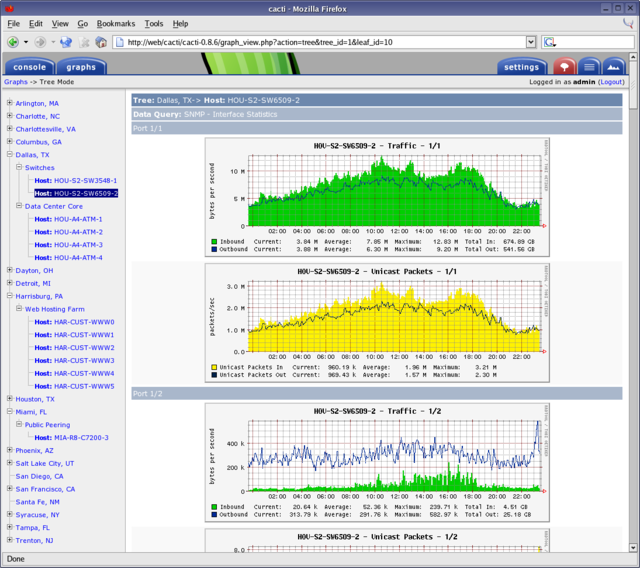
\includegraphics[width=1\textwidth]{img/cacti.png}
}\\[0.1cm]
\end{center}
\end{figure}


Dostawca danych jest to element systemu, który jest odpowiedzialny za
faktyczne wykonywanie sprawdzeń danej wartości i~przekazywanie ich do
narzędzia RRDTool. System umożliwia wybór jednego z~dwóch dostawców
danych. Pierwszym z~nich jest cmd.php, który jest prostym skryptem
napisanym w języku php. Umożliwia on monitorowanie aktywne urządzeń
przy pomocy protokołu SNMP\footnote{ {\em Simple Network Management
    Protocol} -- protokół zarządzania urządzeniami sieciowymi
  i~uzyskiwania informacji o~ich stanie. Zorganizowany w~formie
  drzewa, gdzie każdy liść posiada globalnie unikalny identyfikator
  o~ściśle określonym znaczeniu. Szeroko opisany w \cite{www:SNMP}.}. Skrypt
cmd.php przeznaczony jest do monitorowania jedynie niewielkich
sieci. Ze względów wydajnościowych, nie jest możliwe wykorzystanie go
do monitorowania rozległej infrastruktury.

Drugim z~możliwych do wyboru dostawców danych jest program Spine,
nazywany również Cacttid. Jest to program napisany w~języku~C, który
uruchomiony jest jako serwis systemowy na urządzeniu
monitorującym. Umożliwia on monitorowanie urządzeń zarówno poprzez
protokół SNMP jak i~z~wykorzystaniem innych metod. Możliwość
dostarczenia własnych metod monitorowania opiera się na dostarczeniu
skryptu lub pliku wykonywalnego, który będzie cyklicznie uruchamiany
przez Cactid, a~jako wyniki przekazywane w taki sam sposób jak
z~sprawdzeń operlających się na SNMP.

Żaden z~dostawców danych nie umożliwia monitorowania danego urządzenia
lub usługi w~sposób pasywny. Cacti nie posiada również żadnego
mechanizmu, który pozwoliłby na monitorowanie sieci w~sposób
rozproszony. Oznacza to, iż administrator musi zmienić konfigurację
sieci, tak aby jeden serwer miał dostęp do każdego urządzenia, lub
konfigurować i~zarządzać osobną instancją w~każdym serwerze. Jest to
bardzo niewygodne i~wręcz uniemożliwia monitorowania rozległych sieci
przy pomocy Cacti\footnote{Więcej informacji na temat systemu
  monitorowania Cacti można znaleźć w~\cite{www:Cacti}.}.

\subsection[Nagios][System monitorowania Nagios]{System monitorowania Nagios}

System Nagios został opublikowany w~1999 na licencji GPL. System od
niemal 15 lat jest ciągle rozwijany i~udoskonalany, zarówno przez
autorów jak i~przez szeroką społeczność. W~systemie Nagios najwyższym
priorytetem jest dbałość o~zapewnienie dostępności wszystkich
monitorowanych usług. Organizacja systemu zakłada, iż w~sieci znajdują
się urządzenia, które mogą świadczyć pewne usługi. Każde urządzenie
jak i~usługa może być w jednym z trzech stanów logicznych:

\begin{description}
\item[OK] usługa działa poprawnie
\item[WARNING] monitorowane parametry przekroczyły stan ostrzegawczy
\item[CRITICAL] parametry usługi przekroczyły stan krytyczny, usługa
  lub urządzenie nie funkcjonuje
\end{description}

System posiada rozbudowane algorytmy określania stanu każdego
urządzenia oraz usługi. Działanie usługi, jest zawsze zależne od stanu
urządzenie, na którym dana usługa jest świadczona. Ponadto użytkownik
może definiować zależności pomiędzy urządzeniami. System Nagios
posiada rozbudowany system powiadamiania administratora o~wystąpieniu
awarii oraz o~jej zakończeniu, lub innych zdefiniowanych wydarzeniach
systemowych. Ponadto możliwe jest automatyczne wykonywanie
zdefiniowanych programów lub skryptów, jeśli wystąpiło jakieś
zdarzenie. Podstawowa wersja systemu składa się z następujących
elementów:

\begin{itemize}
\item Interfejs graficzny
\item Rdzeń monitorujący
\end{itemize}

Interfejs graficzny został napisany w~języku~C z~wykorzystaniem
technologi CGI\footnote{{\em Common Gateway Interface} --
  znormalizowany interfejs służący do komunikacji pomiędzy serwerem
  www, a~zewnętrznymi programami. Interfejs ten jest wykorzystywany do
  generowania stron internetowych na żądanie klienta. Zewnętrzny
  program generuje stronę w~języku HTML, a~następnie serwer przesyła
  ją do klienta. Szczegółowy opis można znaleźć w~\cite{www:CGI}}. Jego wygląd
jest zgodny z~standardami z~lat 90. Klasyczna strona WWW bez
dynamicznie zmieniającej się treści. Dane odświeżane są na żądanie
klienta, lub co określony czas. Wykorzystana technologia zakłada
przesyłanie za każdym razem całego dokumentu HTML do klienta,
w~związku z~czym generowany jest nadmierny ruch sieciowy. Widok
użytkownika składa się z~kliku części. Po lewej stronie widoczne jest
klasyczne menu, umożliwiające użytkownikowi wybór treści. Na górze
strony natomiast znajduje się podsumowanie aktualnego stanu
monitorowanych urządzeń i~usług. Centralną część okna zajmuje pulpit,
który prezentuje użytkownikowi treść wybraną wcześniej
z~menu. Interfejs użytkownika umożliwia podgląd aktualnego stanu usług
oraz urządzeń. Informacja ta może być wyświetlana w~formie listy
zawierającej urządzenie i~usługi, lub w~postaci mapy sieci, która
pozwala na monitorowanie stanu urządzenia w~korelacji z~jego logicznym
umieszczeniem w~strukturze sieciowej. Możliwe jest również
przeglądanie historii awarii oraz prostych wykresów zależności stanu
urządzenia lub usługi w~zadanym przedziale czasu. Dostęp do interfejsu
chroniony jest przy pomocy autoryzacji uwierzytelnienia http. Możliwe
jest definiowanie wielu użytkowników, jednak tylko z~poziomu
urządzenia na którym uruchomiony jest system monitorujący. Należy
zauważyć również, że wszyscy użytkownicy posiadają takie same
uprawnienia do wyświetlania danych oraz zarządzania.

%czy prawa autorskie?
\begin{figure}[h]
\label{fig:NagiosInterface}
\caption{Interfejs użytkownika systemu Nagios.}
\begin{center}
\makebox[\textwidth]{%
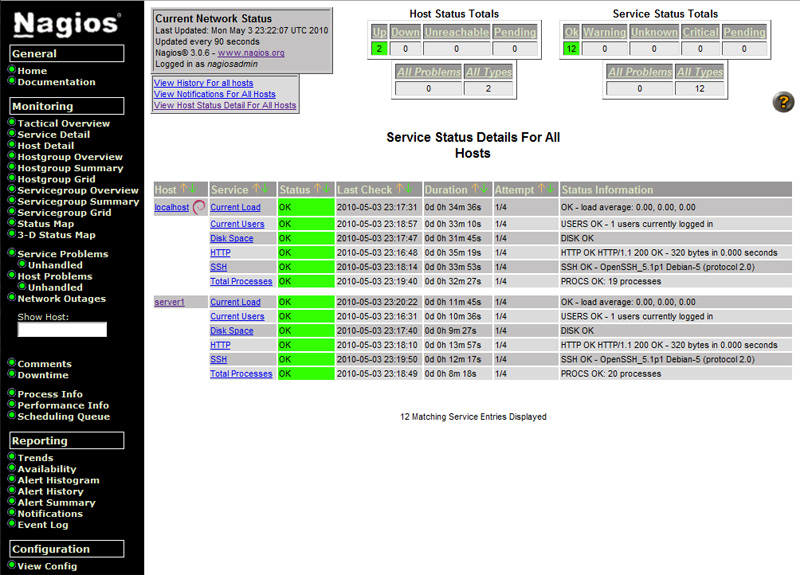
\includegraphics[width=1\textwidth]{img/nagios.jpg}
}\\[0.1cm]
\end{center}
\end{figure}

Rdzeń monitorujący został zaimplementowany w~języku C. Jest to centrum
całego systemu, gdyż zajmuje się on przetwarzaniem wszystkich
bieżących danych monitorowania, a~następnie składowaniem ich
w~plikach. Ta cześć systemu jest odpowiedzialna za wykonywanie
sprawdzeń w~określonych odstępach czasu. Każde sprawdzenie odbywa się
poprzez wykonanie komendy zdefiniowanej przez użytkownika. Komenda ta
może zawierać zarówno wykonanie pliku binarnego jak i~dowolnego
skryptu. W~ramach projektu Nagios, rozwijany jest zestaw
wtyczek\footnote{Należy zwrócić uwagę na różne znaczenie słów wtyczka
  (ang. {\em Plugin}) oraz dodatek (ang. {\em Addon}). }, czyli
programów służących do monitorowania podstawowych usług oraz
parametrów urządzeń. Dostępna jest bardzo duża liczba wtyczek, dzięki
czemu system Nagios może monitorować w~sposób aktywny wszystkie
podstawowe parametry lub usługi. Możliwe jest również definiowanie
własnych wtyczek, które będą sprawdzały stany pewnych specyficznych
dla danej sieci parametrów. W~celu zapewnienia poprawnego
funkcjonowania całego systemu, konieczne jest, aby dodatkowe wtyczki
spełniały wymagania opisane w~\cite{www:NagiosPluginsTutorial}. System
umożliwia również monitorowanie dowolnych usług w~sposób
pasywny. Programy dostarczające odczytów pasywnych również są
zobowiązane do przestrzegania wcześniej wspomnianych zasad.

\begin{figure}[h]
\label{fig:NagiosInterface}
\caption{Interfejs użytkownika systemu Icinga.}
\begin{center}
\makebox[\textwidth]{%
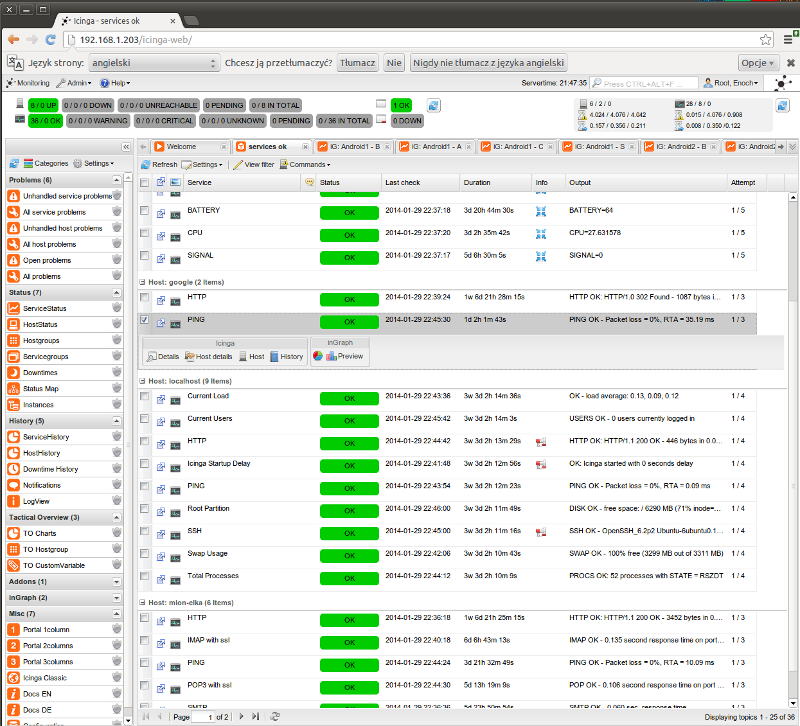
\includegraphics[width=1\textwidth]{img/icinga.png}
}\\[0.1cm]
\end{center}
\end{figure}

System posiada rozbudowane możliwości monitorowania
rozproszonego. Niestety, do wykonania znacznej części z~tych
konfiguracji potrzebne są elementy systemu, które są dystrybuowane za
opłatą. Istnieją również darmowe dodatki, które pozwalają na
przechowywanie zgromadzonych danych zarówno w~bazie relacyjnej jak
i~cyklicznej. Możliwa jest również częściowa integracja systemu
Nagios\footnote{Szczegółowe informacje na temat rozszerzania
  funkcjonalnosci oraz samego systemu można znaleźć
  w~\cite{www:Nagios}.}  z~dodatkami lub systemami, które pozwalają na
wizualizacje zgromadzonych danych.

\subsection[Icinga][System monitorowania Icinga]{System monitorowania Icinga}
\label{subsec:Icinga}

System Icinga powstał w 2009 roku jako klon (ang. fork) systemu
Nagios. System został wzbogacony o~wiele nowych elementów, a~także
poprawiono wiele błędów obecnych w~systemie Nagios. Dzięki zachowaniu
wstecznej kompatybilności zarówno wszystkie wtyczki jak i~dodatki
systemu Nagios mogą być wykorzystane w~systemie Icinga. Pozyskano temu
bardzo dużą bazę wtyczek, co umożliwia monitorowanie tych samych usług
i~urządzeń co przodek.

System Icinga został wyposażony w zupełnie nowy interfejs
graficzny\footnote{Skorzystanie z nowego interfejsu wymaga użycia
  modułu IDOUtils oraz bazy danych. Możliwe jest wykorzystanie również
  klasycznego interfejsu, który nie posiada takich wymagań.}. Został
on zaimplementowany w języku PHP przy użyciu szkieletu aplikacji
agavi\footnote{{\em Agavi } -- szkielet aplikacji języka PHP5
  pozwalający na łatwą realizację funkcjonalnośći zgodne z modelem
  programowym Model-Widok-Kontroler. Szerszy opis znajduje się na
  stronie domowej projektu: \cite{www:Agavi}}. Jest on zatem oparty na
technologii Ajax, dzięki której komunikacja z~użytkownikiem, nie opera
się na przesyłaniu całych stron w~języku HTML, lecz na realizacji
żądań generowanych poprzez język skryptowy wykonywany po stronie
użytkownika. Dzięki zastosowaniu tej technologi, proces wyświetlania
strony zużywa mniejszą część pasma, a~serwer został odciążony. Nowy
interfejs użytkownika jest w~pełni dynamiczny, składa się on
z~rozszerzalnego menu po lewej stronie oraz pulpitów użytkownika
w~centralnej części. Możliwe jest otwieranie wielu pulpitów oraz
wyświetlanie poszczególnych informacji w~osobnych oknach, które można
swobodnie przemieszczać w~obszarze strony. Przykładowy pulpit dostępny
dla użytkownika został przedstawiony na
\ref{fig:IcingaInterface}.Znacznej zmianie uległ również model
bezpieczeństwa. W~nowym interfejsie graficznym, każdy użytkownik,
posiada swój zestaw zdefiniowanych uprawnień. Oznacza to, że możliwe
jest ograniczenie użytkownikowi dostępu do danych o~konkretnej usłudze
lub zabronić wykonywania niektórych czynności
administracyjnych. Zarządzanie użytkownikami oraz ich uprawnieniami
możliwe jest również z~poziomu graficznego interfejsu użytkownika, co
znacząco podnosi wygodę użytkowania systemu.

Kolejną istotną różnicą, jest zmiana architektury systemu. System
Nagios posiada budowę monolityczną, a~współpraca pomiędzy
poszczególnymi jego komponentami odbywa się w~sposób bardzo zawiły
i~niejednorodny. System Icinga wprowadził natomiast budowę
modularną. Wszystkie możliwe komponenty systemu zostały wyodrębnione,
a~do swobodnej komunikacji pomiędzy nimi zdefiniowano wygodne
API. Taka budowa umożliwia przede wszystkim rozmieszczenie
poszczególnych komponentów systemu na różnych fizycznych maszynach, co
w~przypadku dużych sieci może spowodować znaczący wzrost wydajności
i~niezawodności. Dostarczenie jednolitego REST API\footnote{ang. {\em
    Representational state transfer} -- lekka metoda przesyłania
  danych pomiędzy klientem a~serwerem.} umożliwia również prostsze
tworzenie dodatków rozbudowujących możliwości systemu.  W~systemie
Icinga rozbudowano także możliwości współpracy z~bazą danych. System
ten umożliwia współpracę, już nie tylko z~bazą MySQL, lecz również
z~bazami PostgreSQL czy też z~systemem zarządzania bazą danych firmy
Oracle. Możliwość wykorzystania bazy danych Oracle, jest bardzo
istotna, jeśli dane dotyczące pomiarów muszą być przechowywane przez
długi czas, lub jeśli monitorowana infrastruktura jest bardzo
rozbudowana.

System Icinga, nie tylko umożliwia rozmieszczenie modułów na różnych
fizycznych maszynach, lecz również umożliwia wiele innych
konfiguracji, które można wykorzystać podczas monitorowania
rozproszonego. Szczególnie wartą zauważenia jest konfiguracja,
w~której występuje wiele równorzędnych instancji rdzenia
monitorującego, natomiast wszystkie współpracują używając jednej bazy
danych. Centralna baza danych stanowi źródło danych dla interfejsu
graficznego. Taka konfiguracja umożliwia monitorowanie bardzo rozległej
lub wielosegmentowej infrastruktury. Należy również nadmienić, iż
wszystkie elementy niezbędne do konfiguracji takiego rozwiązania są
darmowe.

\section[Podsumowanie][Podsumowanie]{Podsumowanie}

Współczesne systemy monitoringu, są bardzo bogato wyposażone
i~posiadają szereg zaawansowanych możliwości. Każdy z~systemów oferuje
unikalny zestaw rozwiązań, które z~pewnością mogą zostać wykorzystane
w~wielu instytucjach. Porównując wszystkie omówione systemy, należy
zwrócić szczególną uwagę, na różnice w~ich możliwych zastosowaniach
docelowych.

Systemy, takie jak Cacti zaliczane są do grupy systemów
analitycznych. Ich celem jest zatem zapewnienie możliwości
gromadzenia oraz analizy danych. Zbierane dane mają charakter
pojedynczych, dokładnych wartości, na podstawie których prezentowane
są użytkownikowi odpowiednie wykresy. Niestety ze względu na sposób
gromadzenia danych - protokół SNMP, oraz ubogość metod ich gromadzenia
systemy te, nie mogą być wzbogacone o~funkcjonalność charakterystyczną
dla systemów dostępnościowych.

Drugą grupę systemów stanowią natomiast systemy dostępnościowe, takie
jak Nagios czy Icinga. Ich głównym celem jest monitorowanie bieżącego
stanu infrastruktury i~raportowanie użytkownikowi najświeższych
informacji. Systemy te zostały również zaprojektowane, aby wspomagać
administratora w~lokalizacji awarii. Głównym typem danych na których
operują te systemy jest stan urządzenia lub usługi. Zdefiniowanie
odpowiednich poziomów kwantyzacji dla stanów pozwala na szybkie
uzyskiwanie poglądowych informacji o~stanie sieci. Podczas
monitorowania gromadzone są również dane szczegółowe. Ich
przetwarzaniem nie zajmują się już jednak same systemy monitorowania,
lecz liczne dodatki do nich. Możliwe jest zatem rozbudowanie systemu
tego typu, o~dodatkowe elementy, które pozwolą uzyskać system
hybrydowy. System taki będzie mógł pełnić rolę zarówno systemu
dostepnościowego jak i analitycznego.

Wybierając system monitorujący, należy zatem dokonać szczegółowej
analizy wymagań stawianych przed systemem. Szczegółowe porównanie
wszystkich przedstawionych systemów monitorowania zawarto
w~\ref{tab:PorownanieSys}.

\begin{longtable}[c]{|p{4.5cm}||p{3cm}|p{3cm}|p{3cm}|}
  \caption[Porównanie systemów monitorowania]{Porównanie systemów monitorowania} \label{tab:PorownanieSys} \\
  \hline \multicolumn{1}{|c||}{Nazwa systemu} &
  \multicolumn{1}{c|}{Cacti} & \multicolumn{1}{c|}{Nagios} &
  \multicolumn{1}{c|}{Icinga} \tabularnewline \hline \hline
  \endfirsthead

  \multicolumn{4}{c}%
  {{\tablename\ \thetable{} -- Kontynuacja z~poprzedniej strony}} \\
  \hline
  \multicolumn{1}{|c||}{Nazwa systemu} &
  \multicolumn{1}{c|}{Cacti} & \multicolumn{1}{c|}{Nagios} &
  \multicolumn{1}{c|}{Icinga} \tabularnewline 
  \hline \hline
  \endhead

  \hline \multicolumn{4}{|r|}{{Kontynuacja na następnej stronie}} \\ \hline
  \endfoot

  \hline\hline
  \endlastfoot

  \raggedright{Podgląd stanu bieżącego} & \raggedright{Nie} &
  \raggedright{Ta}k & \raggedright{Ta}k \tabularnewline 
  \hline

  \raggedright{Podgląd danych historycznych} &\raggedright{Tak} &
  \raggedright{Tak, przez dodatek} & \raggedright{Tak, przez dodatek}
  \tabularnewline
  \hline

  \raggedright{Dane w~formie wykresu} & \raggedright{Tak} &
  \raggedright{Tak, przez dodatek} & \raggedright{Tak, przez dodatek}
  \tabularnewline 
  \hline

  \raggedright{Przechowywanie danych w~bazie cyklicznej} & \raggedright{Tak} &
  \raggedright{Tak, przez dodatek} & \raggedright{Tak, przez dodatek}
  \tabularnewline
  \hline

  \raggedright{Przechowywanie danych w~bazie relacyjnej} & \raggedright{Nie} &
  \raggedright{Tak, przez dodatek} & \raggedright{Tak, przez dodatek}
  \tabularnewline
  \hline

  \raggedright{Powiadomienia o~awarii} & \raggedright{Nie} &
  \raggedright{Tak, email lub telefon} & \raggedright{Tak, email lub telefon}
  \tabularnewline
  \hline

  \raggedright{Wsparcie w~lokalizacji awarii} & \raggedright{Nie} &
  \raggedright{Tak, poprzez mapę logiczną sieci} & \raggedright{Tak, poprzez mapę logiczną sieci}
  \tabularnewline
  \hline

  \raggedright{Obsługa SNMP} & \raggedright{Tak} &
  \raggedright{Tak, przez wtyczkę} & \raggedright{Tak, przez wtyczkę}
  \tabularnewline
  \hline

  \raggedright{Zbieranie danych spoza SNMP} & \raggedright{Tak, niewielka liczba dostępnych metod} &
  \raggedright{Tak, bogaty zestaw wtyczek} & \raggedright{Tak, bogaty zestaw wtyczek}
  \tabularnewline
  \hline

  \raggedright{Monitorowanie pasywne} & \raggedright{Nie} &
  \raggedright{Tak} & \raggedright{Tak}
  \tabularnewline
  \hline

  \raggedright{Nowoczesny interfejs użytkownika} & \raggedright{Nie} &
  \raggedright{Nie} & \raggedright{Tak, z wykorzystaniem technologi AJAX}
  \tabularnewline
  \hline

  \raggedright{Wielu użytkowników} & \raggedright{Tak} &
  \raggedright{Tak} & \raggedright{Tak}
  \tabularnewline
  \hline

  \raggedright{Metoda uwierzytelnienia} & \raggedright{Uwierzytelnienie wewnętrzne} &
  \raggedright{Uwierzytelnienie http} & \raggedright{Uwierzytelnienie wewnętrzne}
  \tabularnewline
  \hline

  \raggedright{Zarządzanie kontami użytkowników z~interfejsu} & \raggedright{Tak} &
  \raggedright{Nie} & \raggedright{Tak}
  \tabularnewline
  \hline

  \raggedright{Definiowanie uprawnień dla użytkowników} & \raggedright{Tak, przez interfejs graficzny} &
  \raggedright{Nie} & \raggedright{Tak, przez interfejs graficzny}
  \tabularnewline
  \hline

  \raggedright{Modularność} & \raggedright{Nie} &
  \raggedright{Nie} & \raggedright{Tak}
  \tabularnewline
  \hline

  \raggedright{Rozmieszczenie modułów na różnych urządzeniach fizycznych} & \raggedright{Nie dotyczy} &
  \raggedright{Nie dotyczy} & \raggedright{Tak}
  \tabularnewline
  \hline

  \raggedright{Możliwość monitorowania rozproszonego z~instancją
    nadrzędną} & \raggedright{Nie} & \raggedright{Tak} &
  \raggedright{Tak}
  \tabularnewline
  \hline

  \raggedright{Możliwość monitorowania rozproszonego bez instancji nadrzędnej} & \raggedright{Nie} &
  \raggedright{Tak, konieczny płatny dodatek} & \raggedright{Tak}
  \tabularnewline
  \hline

  \raggedright{Generacja raportów} & \raggedright{Nie} &
  \raggedright{Nie} & \raggedright{Tak, z~wykorzystaniem JasperReports}
  \tabularnewline
  \hline

  \raggedright{Możliwość monitorowania klienta mobilnego} & \raggedright{Nie} &
  \raggedright{Nie} & \raggedright{Nie}
  \tabularnewline
  \hline

  \raggedright{Dostępność} & \raggedright{Darmowy} &
  \raggedright{Częściowo darmowy, wiele płatnych elementów i~funkcjonalności} & \raggedright{Darmowy}
  \tabularnewline
  \hline

  \raggedright{Licencja} & \raggedright{GPL v2} &
  \raggedright{GPL v3 (tylko darmowe elementy)} & \raggedright{GPL v2}
  \tabularnewline
  \hline

\end{longtable}

Przedstawione systemy monitorujące w~znacznym stopniu zaspokajają
zapotrzebowanie rynku na systemy monitorowania. Pojawia się jednak
pewna nisza związana z~monitorowaniem urządzeń mobilnych. Zadanie to
nie jest trywialne i~wymaga obecności dodatkowych mechanizmów zarówno
na urządzeniu mobilnym, jak i~w~innych elementach systemu. Żaden
z~analizowanych systemów nie posiadał w~swej implementacji ani
w~oficjalnych repozytoriach z~dodatkami, oprogramowania, które
pozwalałoby na monitorowanie parametrów urządzenia mobilnego.


%\chapter{Rodzaje systemów monitorujących}

\section[Systemy aktywne][Systemy aktywne]{Systemy aktywne}

\section[Systemy pasywne][Systemy pasywne]{Systemy pasywne}



\chapter{Monitorowanie klienta mobilnego jako monitorowanie rozproszone}
\label{chap:Wymagania}
\section[Charakterystyka problemu][Charakterystyka problemu]{Charakterystyka opoblemu}

\section[Wymagania funkcjonalne][Wymagania funkcjonalne]{Wymagania funkcjonalne}

\section[Wymagania niefunkcjonalne][Wymagania niefunkcjonalne]{Wymagania niefunkcjonalne}

\chapter{System monitorowania Icinga}
\label{chap:Icinga}

\section[Opis systemu][Opis systemu]{Opis systemu}

System Icinga powstał jako klon systemu Nagios. Zachowana została
kompatybilność wsteczna przez co możliwe jest używanie dodatków oraz
wtyczek przeznaczonych dla systemu Nagios. Podstawowa konfiguracja
systemu Icinga składa się dwóch modułów:

\begin{itemize}
\item Rdzeń monitorujący
\item Interfejs użytkownika
\end{itemize}

Rdzeń monitorujący stanowi element centralny całego systemu. Do jego
zadań należy przede wszystkim monitorowanie usług i~urządzeń zgodnie
z~ustawieniami zawartymi w~plikach konfiguracyjnych. System posiada
możliwość monitorowania zarówno aktywnego jak
i~pasywnego. Monitorowanie aktywne wykonywane jest przy pomocy
zewnętrznych programów lub skryptów nazywanych wtyczkami. Każda usługa
oraz urządzenia posiada zdefiniowaną komendę sprawdzającą która
definiuje jaką wtyczkę należy uruchomić oraz jakie dane do niej
przekazać. Każda wtyczka posiada zdefiniowany zestaw danych
wejściowych, które odpowiadają jej opcjom konfiguracyjnym. Po
zakończeniu pomiaru wtyczka przekazuje dane o~jego wynikach do systemu
monitorującego. Przekazanie to odbywa się dwiema drogami. Pierwsza
z~nich to wartość zwrócona z~programu, która determinuje w~jakim
stanie znajduje się urządzenie lub usługa. Zwrócona wartość powinna
być jedną z następujących:

\begin{description}
\item[0] OK, wtyczka mogła wykonać sprawdzenie i~usługa lub urządzenie
  jest w~stanie OK
\item[1] WARNING, wtyczka mogła wykonać sprawdzenie ale parametry
  urządzenia lub usługi przekraczają poziom ostrzegawczy.
\item[2] CRITICAL, wtyczka mogła wykonać sprawdzenia ale parametry
  urządzenia lub usługi przekraczają poziom krytyczny.
\item[3] UNKNOWN, wtyczka nie była w~stanie wykonać sprawdzenia ze
  względu na dostarczenie nie prawidłowych parametrów wywołania lub
  niskopoziomowego błędu systemu.
\end{description}

Większość wtyczek dokonuje pewnych pomiarów, dlatego każde ich
wykonanie gromadzi zdecydowanie więcej danych niż można przekazać
poprzez jedną z~czterech wartości. Przekazanie pozostałych informacji
odbywa się poprzez dane tekstowe, wypisywane przez wtyczkę na
standardowym wyjściu programu. Dane te rozdzielane są znakiem~| na dwie
grupy. Przed tym znakiem, znajdują się dane czytelna dla człowieka. Po
znaku znajdują się dane wydajnościowe w~formacie klucz=wartość,
przeznaczone do analizy przez zewnętrzne programy np. do generacji
wykresów. Znak~| oraz druga grupa nie są obowiązkowe.

System Icinga umożliwia również monitorowanie w~sposób
pasywny. Dostarczanie wyników sprawdzenia pasywnego odbywa się poprzez
plik komend zewnętrznych. Plik komend zewnętrznych jest to potok
nazwany przez który poszczególne komendy trafiają do rdzenia
monitorującego. Pełna lista dostępnych komend znajduje się
w~\cite[412-436]{www:IcingaDoc}. Zatem pewien dowolny program wykonuje
sprawdzenia urządzenia lub usługi, po czym zapisuje wynik tego
sprawdzenia zgodnie z~formatem do potoku. Format przekazywanego
rezultatu sprawdzenia został opisany
w~\cite[296-299]{www:IcingaDoc}. Jeśli program wykonuje się na
urządzeniu innym niż to na którym uruchomiony jest rdzeń monitorujący
konieczne jest przesłanie danych do tego systemu. System Icinga
posiada do tego celu dodatek NSCA, który został szeroko opisany
w~\ref{sec:NSCA}

Dane otrzymane od wtyczki są przez system monitorujący przechowywane
wraz z~innymi danymi potrzebnymi do monitorowania w~plikach, a~gdy
przestają one być potrzebne, są kasowane. System Icinga udostępnia
jednak możliwość przechowywania tych danych w~bazie danych przy pomocy
komponentu systemu IDOUtils. Został on dokładnie opisany
w~\ref{sec:IDOUtils}. Rdzeń monitorujący posiada także możliwość
udostępniania danych wydajnościowych otrzymanych przez każdą wtyczkę
dla zewnętrznych programów. Możliwe jest zdefiniowanie formatu danych
wyjściowych. Po włączeniu eksportu danych wydajnościowych, rdzeń
monitorujący będzie zapisywał do zdefiniowanych plików dane
wydajnościowe pochodzące od wtyczek jak i~czasy ich przybycia. Dane te
są wykorzystywane np. przez dodatek inGraph opisany
w~\ref{sec:inGraph}.

System Icinga odziedziczył po systemie Nagios klasyczny interfejs
oparty na~technologii CGI. Ponieważ technologia ta jest już
przestarzała, udostępniono użytkownikom również w~pełni nowoczesny
interfejs nazywany icinga-web. Jest to dynamiczny interfejs
użytkownika zaimplementowany w~języku PHP przy wykorzystaniu
technologii AJAX. Różnice pomiędzy tymi interfejsami zauważalne są nie
tylko w~warstwie prezentacji lecz również w~architekturze i~warstwie
komunikacji z~rdzeniem monitorującym. Interfejs klasyczny
wykorzystywał pliki generowane przez rdzeń monitorujący do pobierania
aktualnych danych, przez co musiał on znajdować się na tym samym
urządzeniu co rdzeń monitorujący. W~przypadku interfejsu icinga-web
komunikacja z~rdzeniem monitorującym odbywa się poprzez bazę danych,
dzięki czemu elementy te mogą znajdować się na różnych fizycznych
urządzeniach. Ponadto interfejs ten wykorzystuje drugą bazę danych
o~bardzo prostym schemacie jako miejsce przechowywania danych
konfiguracyjnych. Należy również dostrzec różnice
w~bezpieczeństwie. Interfejs klasyczny zabezpieczony był jedynie
poprzez mechanizm uwierzytelnienia http i~wszyscy użytkownicy mieli
dostęp do całego systemu. Interfejs icinga-web posiada swoją bazę
użytkowników oraz ich uprawnień. Umożliwia to ograniczenie praw danego
użytkownika np. tylko do wyświetlania stanu konkretnego urządzenia lub
usługi.

\section[Komponent IDOUtils][Komponent IDOUtils]{Komponent IDOUtils}
\label{sec:IDOUtils}

Komponent IDOUtils jest to zestaw programów dzięki którym możliwe jest
składowanie informacji generowanych przez rdzeń monitorujący w~bazie
danych. W~wersji dostępnej podczas pisania tej pracy wspierany były
następujące systemy zarządzania bazą danych:

\begin{itemize}
\item MySql,
\item PostgreSQL,
\item Oracle.
\end{itemize}

W~celu zapewnienia funkcjonalności omawianego komponentu, konieczne
jest utworzenie bazy danych o~odpowiednim schemacie, który został
opisany w~\cite[669-750]{www:IcingaDoc}. Udostępnione zostały również
skrypty SQL, które definiują odpowiednie tabele. Ponadto administrator
musi zapewnić odpowiednia konfigurację bazy danych, w~tym konto
użytkownika i~hasło, w~taki sposób, aby umożliwić odpowiednim
elementom komponentu IDOUtils dostęp do bazy danych.

W~celu odciążenia urządzenia, na którym uruchomiony jest system
Icinga. Komponent ten został podzielony, na kilka elementów, które
mogą znajdować się na różnych urządzeniach. Można wyróżnić następujące
elementy:

\begin{description}
\item[IDOMOD] moduł rdzenia monitorującego, który pozwala mu na dostęp
  do bazy danych
\item[LOG2IDO] program pozwalający na import utworzonych wcześniej
  plików do bazy danych
\item[FILE2SOCK] program pozwalający na przekierowanie danych
  zapisywanych do pliku do gniazda TCP lub Unix
\item[IDO2DB] demon, który jest odpowiedzialny za wykonywanie operacji
  na bazie danych
\end{description}

Podstawowymi elementami całego komponentu są IDOMOD oraz IDO2DB. Moduł
rdzenia IDOMOD ładowany jest przez rdzeń systemu Icinga tuż po
starcie. Po załadowaniu zapewnia on spójny interfejs do uzyskiwania
danych dla wszystkich pozostałych części rdzenia
monitorującego. Ponieważ wykonywanie operacji na bazie danych może być
czasochłonne nie powinno być to wykonywane przez rdzeń
monitorujący. Z~tego powodu powstał program IDO2DB. Jest on
uruchomiony jako demon na dowolnym urządzeniu. Zadaniem tego serwisu
jest fizyczna realizacja żądań na bazie danych.

Ponieważ rdzeń monitorujący oraz demon IDO2DB mogą znajdować się
zarówno na jednym urządzeniu jak i~na różnych urządzeniach konieczne
jest zapewnienie odpowiednich mechanizmów komunikacji pomiędzy nimi.
Gdy programy te znajdują się na różnych urządzeniach, jako mechanizm
komunikacji wykorzystywane są gniazda TCP. W~podstawowej konfiguracji
dane przekazywane są w~sposób niezaszyfrowany. Jeśli jednak istnieje
potrzeba zapewnienia tajności oraz integralności przekazywanych danych
możliwe jest użycie protokołu SSL\footnote{ ang. {\em Secure Socket
    Layer} -- protokół warstwy prezentacji, zapewniający poufność oraz
  integralność przesyłanych danych.}. W~sytuacji, gdy oba programy
uruchomione są na tym samym urządzeniu, w~celu poprawy wydajności
możliwe jest użycie gniazd protokołu Unix\footnote{ and. {\em Unix
    Domain Socket} -- metoda komunikacji między procesowej w~systemach
  Unix. Posiada jednolite API jak gniazda domeny
  internetowej.}. Najpopularniejszy sposób użycia został przedstawiony
schematycznie na~\ref{fig:IDOUtils}.

\begin{figure}[ht]
  \caption{Schemat wykorzystania IDOUtils w systemie Icinga.}
  \label{fig:IDOUtils}
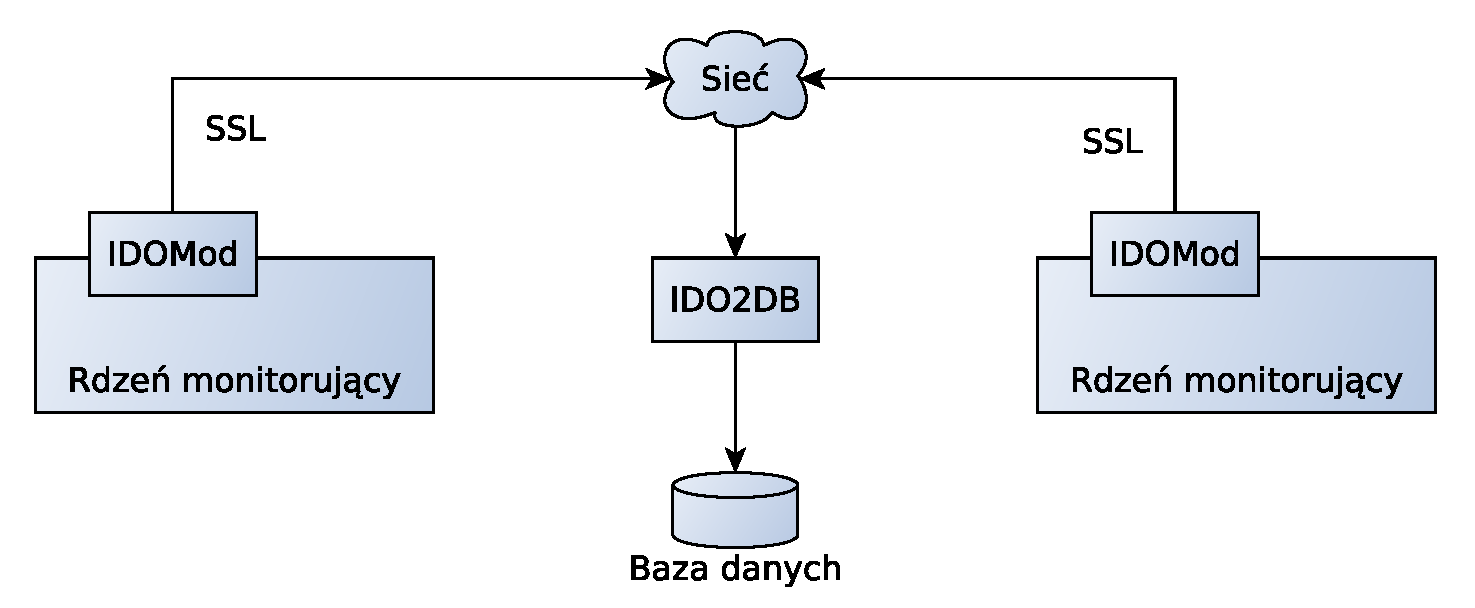
\includegraphics[width=1\textwidth]{img/idoutils}
\end{figure}

W~celu zapewnienia możliwości migracji z~środowiska, które korzystało
wcześniej z~przechowywania danych w~plikach, został dostarczony
program LOG2IDO. Pozwala on, na import danych historycznych do bazy
danych. Program ten, analogicznie jak IDOMOD nie operuje bezpośrednio
na bazie danych, lecz komunikuje się tymi samymi metodami co IDOMOD
z~demonem IDO2DB. Zarówno program LOG2IDO jak i~moduł IDOMOD mogą
kierować żądania do IDO2DB poprzez plik. W~celu zapewnienia
przekazywania tych danych z~pliku do demona IDO2DB opracowano program
FILE2SOCK. Jest to prosty program, który przekazuje dane zapisane do
danego pliku do demona IDO2DB. Program ten nie zajmuje się w~żadnym
stopniu przetwarzaniem odczytaniem danych, lecz jedynie przesłaniem ich
poprzez gniazdo internetowe lub Unix do demona IDO2DB.

\section[Dodatek inGraph][Dodatek inGraph]{Dodatek inGraph}
\label{sec:inGraph}

inGraph jest to dodatek do systemów Icinga oraz Nagios, który
umożliwia prezentację danych zgromadzonych poprzez system monitorujący
w~postaci wykresów. Dodatek ten został opracowany przez firmę NETWAYS
GmbH i~wydany na licencji GPL w~wersji 3. Cechą, która odróżnia
dodatek inGraph od innych rozwiązań, przeznaczonych do analizy danych
historycznych jest wykorzystanie relacyjnej bazy danych do
przechowywania danych otrzymanych od systemu monitorującego. Dane, Na
podstawie otrzymanych danych dodatek inGraph dokonuje przeliczeń dla
odpowiednich przedziałów czasowych, które używane są do późniejszej
generacji wykresów. Rozmiary przedziałów definiowane są przez
użytkownika w plikach konfiguracyjnych. Wykorzystanie tego rodzaju
bazy danych powoduje nieustanny wzrost rozmiaru bazy. W celu
optymalizacji zajętości przestrzeni dyskowej dodatek inGraph
administruje danymi zgodnie z polityką zdefiniowaną w plikach
konfiguracyjnych. Dla każdego przedziału czasowego zdefiniowany jest
również okres przechowywania danych. Dodatek umożliwia przeglądanie
danych dokładnych z najmniejszych przedziałów czasu, jak i~wykresów
długoterminowych prezentujących trendy danej wartości. Ponieważ dane
są bezpośrednio administrowane przez dodatek inGraph, możliwa jest
zmiana czasów przechowywania danych z wskazanych przedziałów nawet w
trakcie działania systemu\footnote{Dla porównania należy przypomnieć
  systemy oparte na cyklicznych baza danych, gdzie rozmiar definiowany
  może być tylko i wyłącznie podczas tworzenia bazy.}.

Dodatek inGraph składa się z~dwóch niezależnych elementów,
komunikujących się poprzez XML-RPC\footnote{ang. {\em XML Remote
    Procedure Call} -- zdalne wywołanie procedur przy użyciu
  XML. Metoda zdalnego wywoływania funkcji oparta na dokumentach w
  formacie XML. Szczegółowy opis w~\cite{www:XMLRPC}.}:

\begin{itemize}
\item interfejs graficzny,
\item rdzeń zbierający dane.
\end{itemize}

Rdzeń zbierający oraz przetwarzający dane został napisany w~języku
Python. Jego zadaniem jest pobieranie danych od systemu
monitorującego, dokonywanie ich przeliczeń, oraz umieszczanie ich
wyników w~bazie danych. Do pobierania danych z~systemu monitorującego
wykorzystano mechanizm udostępniania danych wydajnościowych. System
monitorujący, musi eksportować dane przy pomocy formatu zrozumiałego
dla dodatku inGraph. Demon zbierający dane dokonuje analizy
otrzymanych danych, a~następnie wykonuje wszystkie niezbędne
obliczenia, a~wyniki zapisuje w~bazie danych MySQL lub
PostgreSQL. Ważną różnicą pomiędzy danymi składowanymi w~tej bazie,
a~danymi przechowywanymi przez system monitorujący jest ich
format. Systemy monitorujące, przechowują w~postaci numerycznej
jedynie skwantowany stan danej usługi lub urządzenia. Dodatek inGraph
przechowuje natomiast w~swojej bazie dane w~postaci już
przetworzonej. Oznacza to iż dokonywany jest rozbiór składniowy
rezultatów pomiarów i~w~bazie danych zapamiętywane są pochodzące
z~tych rezultatów dane w~postaci numerycznej. Typowy przepływ danych
został przedstawiony na~\ref{fig:inGraphFlow}.

\begin{figure}[ht]
  \caption{Typowy przepływ danych przy wykorzystaniu dodatku inGraph.}
  \label{fig:inGraphFlow}
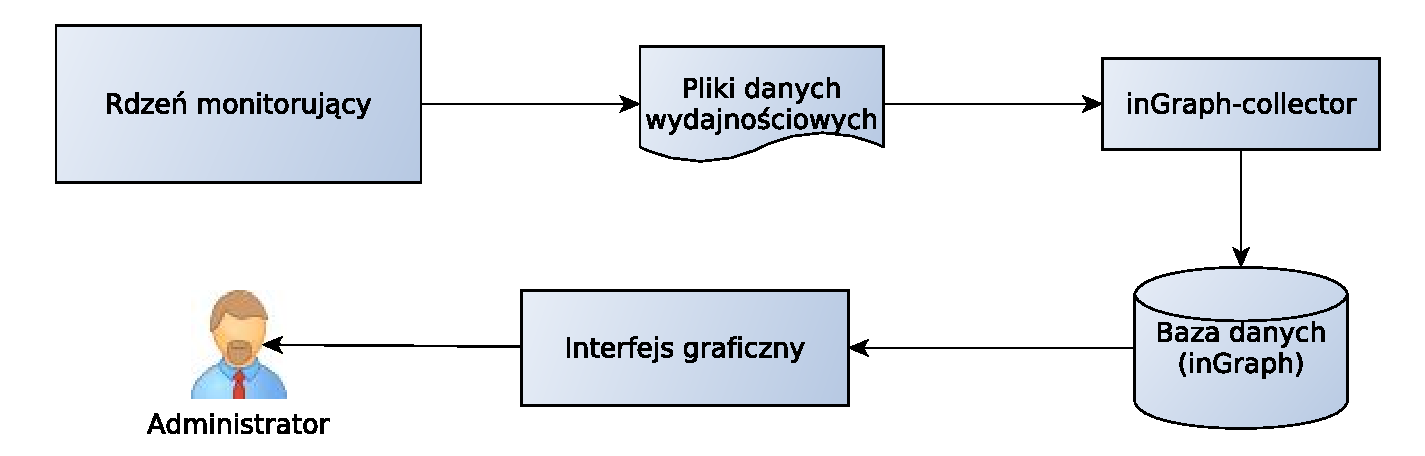
\includegraphics[width=1\textwidth]{img/ingraphFlow}
\end{figure}

Interfejs użytkownika został napisany w~językach PHP oraz
JavaScript. Umożliwia on podgląd danych zebranych i~przetworzonych
przez rdzeń dodatku. Interfejs może funkcjonować zarówno jako
niezależny serwis jak i~jako integralna część interfejsu systemu
Icinga. Umożliwia on generację wykresów dla każdego z~urządzeń oraz
dla każdej z usług. Formaty wykresów, a~także przedziały agregacji
danych definiowane są w~plikach konfiguracyjnych w formacie
JSON\footnote{ang. {\em JavaScrip Object Notation} -- lekki format
  tekstowy wymiany danych komputerowych. Szczegółowo opisany w~\cite{www:JSON}.}.
Użytkownik po wybraniu usługi lub urządzenia uzyskuje interaktywny
wykres przezentujący dane w~zadanym okresie. Wszystkie wykresy
wygenerowane przez program są w~pełni konfigurowalne jak
i~edytowalne. Typ prezentowanych danych jest uzależniony od rozmiaru
przedziału czasu w~którym generowany jest wykres. Jeśli okno czasu
jest odpowiednio małe, na wykresie zostaną przedstawione dane
dokładne. W~sytuacji, gdy nie jest możliwe przedstawienie danych
dokładnych, ze względu na rozmiar zadanego okresu czasu, dane są
agregowane w~przedziały, a~na wykresie udostępniana jest wartość
minimalna, maksymalna oraz średnia dla danego przedziału agregacji
danych. Przykładowe wykresy wygenerowany przy pomocy dodatku inGraph
można zobaczyć na \ref{fig:inGraph}. Szczególną uwagę warto zwrócić na
szare pola reprezentujące minimum oraz maksimum w~danym przedziale.

\begin{figure}[ht]
  \caption{Interfejs dodatku inGraph.}
  \label{fig:inGraph}
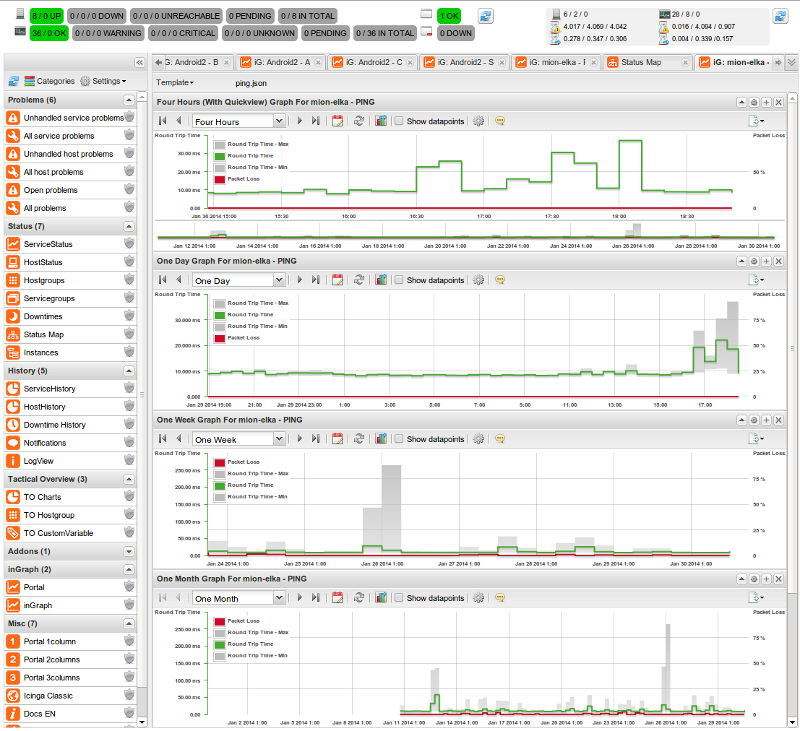
\includegraphics[width=1\textwidth]{img/ingraph.png}
\end{figure}


\section[Dodatek NSCA][Dodatek NSCA]{Dodatek NSCA}
\label{sec:NSCA}

\subsection[Opis dodatku NSCA][Opis dodatku NSCA]{Opis dodatku NSCA}

NSCA - Nagios Service Check Acceptor jest to dodatek do systemów
monitorujących opartych o~system Nagios, więc również systemu
Icinga. Pozwala on na wykorzystanie mechanizmów pasywnego
monitorowania z~systemu innego niż ten na którym uruchomione jest
oprogramowanie monitorujące. Program ten został napisany w~całości
w~języku~C i~wydany na licencji pozwalającej na wgląd do kodu
źródłowego. Wykorzystuje on plik zewnętrznych komend i~nie integruje
się z~rdzeniem monitorującym. Dzięki temu możliwe jest jego
wykorzystanie zarówno w~systemie Nagios jak i~jego klonach takich jak
system Icinga. Dodatek ten składa się z~dwóch modułów:

\begin{itemize}
\item moduł wysyłający (send\_nsca) służący do wysyłania wyników
  sprawdzeń z~monitorującego systemu do centralnego serwera, na którym
  umieszczony jest rdzeń systemu monitorującego odpowiedzialny za
  przetwarzanie wyników sprawdzeń,
\item moduł odbierający (nsca) służący do odbierania wyników sprawdzeń
  od klientów i~dostarczaniu ich do pliku komend zewnętrznych danego
  systemu monitorującego.
\end{itemize}

\begin{figure}[ht]
  \caption{Schemat działania dodatku NSCA.}
  \label{fig:nsca}
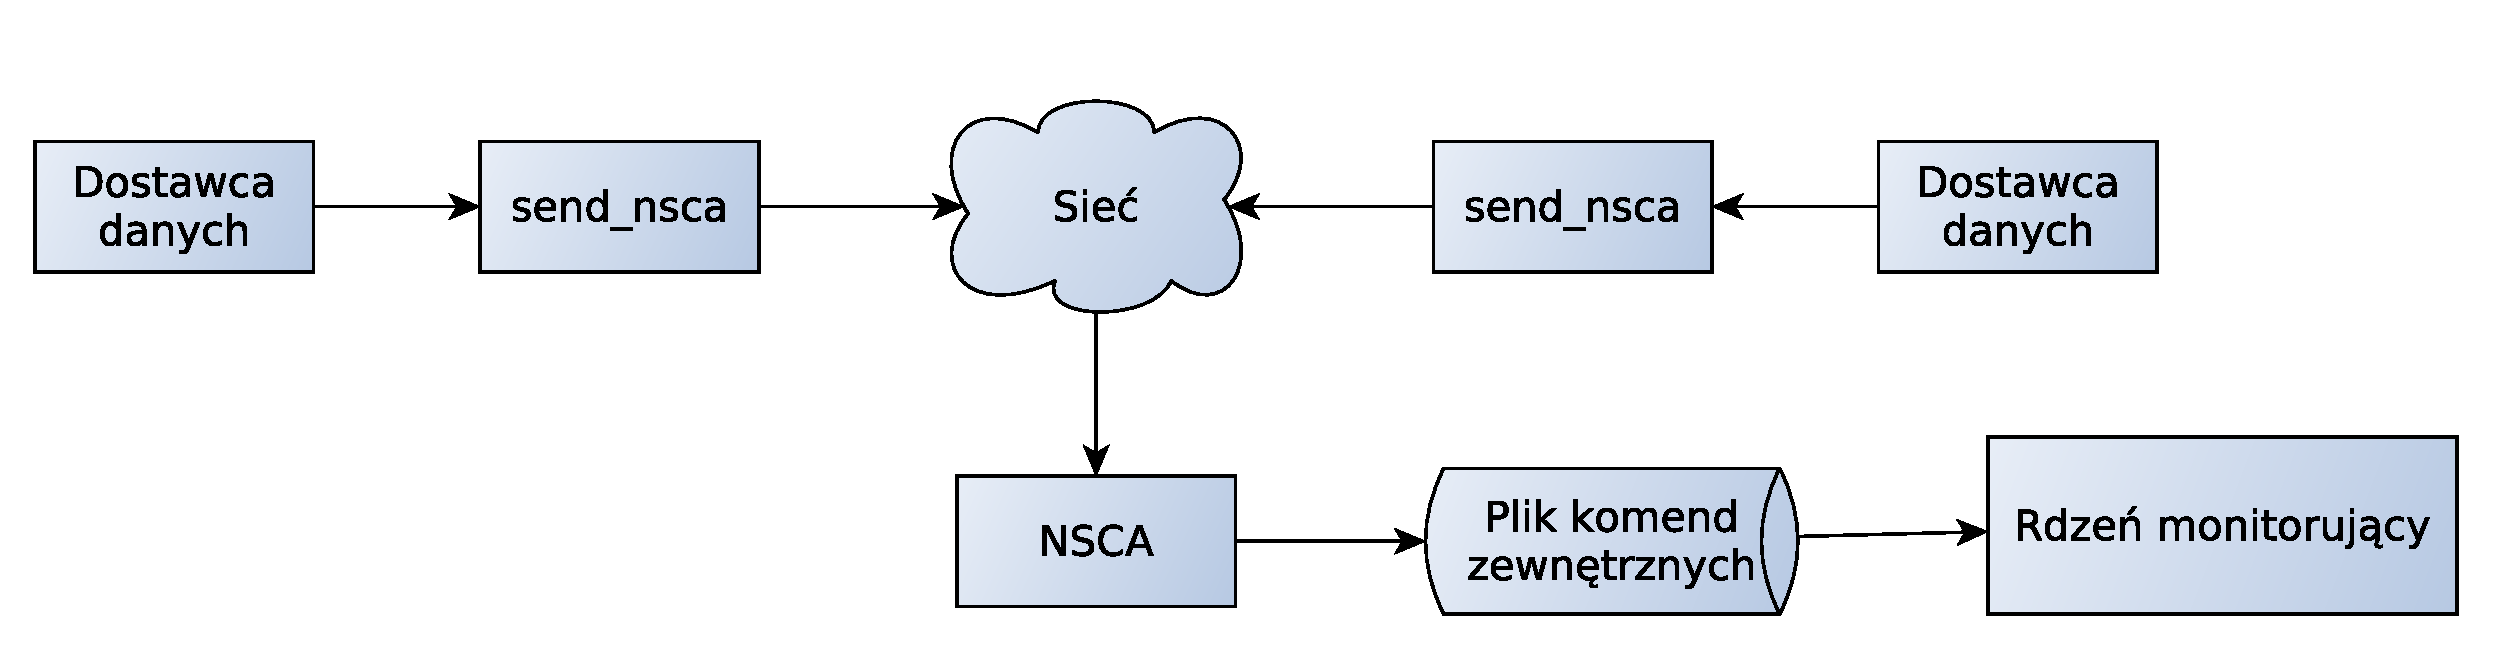
\includegraphics[width=1\textwidth]{img/nsca}
\end{figure}

%źrodło: dokumentacja w repo ?

\subsubsection[Moduł wysyłający][Moduł wysyłający]{Moduł wysyłający}
\label{subsubsec:modulWysylajacy}

Ta część dodatku uruchamiana jest na systemie, na którym funkcjonuje
jakiś mechanizm sprawdzający, który generuje wpisy dziennika. Wpisy te
po utworzeniu, przekazywane są do programu wysyłającego. Moduł
wysyłający, po uruchomieniu odczytuje ustawienia z~pliku
konfiguracyjnego, a~następnie próbuje połączyć się z~serwerem. Po
udanej próbie połączenia otrzymuje pakiet inicjujący, który zawiera:

\begin{description}
\item[wektor inicjujący] używany do celów kryptograficznych,
  wygenerowany przez serwer pseudolosowy ciąg znaków, konieczny do
  inicjalizacji algorytmu kryptograficznego,
\item[stempel czasu] czas odczytany przez serwer w~chwili nadejścia
  połączenia od klienta.
\end{description} 

Po otrzymaniu pakietu inicjującego moduł rozpoczyna czytanie wpisów
z~standardowego wejścia programu. Wszystkie wpisy dziennika muszą być
odpowiednio sformatowane. Poszczególne pola informacyjne muszą być
rozdzielone pojedynczą tabulacją, a~cały wpis zakończony znakiem
nowej linii. Wpisy dotyczącego urządzenia powinny zawierać następujące
pola:

\begin{description}
\item[nazwa urządzenia] krótka nazwa urządzenia, którego stan jest
  przekazywany,
\item[stan] numerycznie wyrażony kod stanu urządzenia,
\item[odczyt] dodatkowe wartości odczytów opisujące stan urządzenia.
\end{description}

Natomiast wpisy dotyczące usługi świadczonej przez to urządzenia, lub
innego rejestrowanego parametru tego urządzenia powinny zawierać
następujące pola:

\begin{description}
\item[nazwa urządzenia] krótka nazwa urządzenia na którym uruchomiona
  jest usługa,
\item[opis usługi] nazwa usługi danego urządzenia, której dotyczy wpis
\item[stan] numerycznie wyrażony kod stanu usługi,
\item[odczyt] dodatkowe wartości odczytów opisujące stan usługi.
\end{description}

Łatwo zauważyć, że żadne z~pól wpisu dziennika nie zawiera stempla
czasu wymaganego przez rdzeń sprawdzający przy zapamiętywaniu odczytu
pasywnego. Dzieje się tak, gdyż program NSCA posiada zdefiniowaną
własną politykę określania czasu wpisu w~dzienniku. Do każdego pakietu
zawierającego wpis dziennika dodawany jest stempel czasu otrzymany
w~pakiecie inicjującym od modułu odbierającego. Właściwy stempel
czasu, który trafia do jadra sprawdzającego nadawany jest natomiast
przez moduł odbierający.

Kolejnym krokiem działania modułu jest obliczenie cyklicznego kodu
nadmiarowego CRC32 dla danego pakietu. Po dołączeniu obliczonego kodu
do pakietu pakiet jest szyfrowany. Algorytm kryptograficzny stosowany do
szyfrowania pakietów został wcześniej zainicjalizowany wektorem
pseudolosowych danych odebranych w~pakiecie inicjalizacyjnym od modułu
odbierającego. Po zaszyfrowaniu dane są wysyłane, a~moduł wysyłający,
bez oczekiwania na potwierdzenie przetworzenia przez serwer,
rozpoczyna przetwarzanie kolejnego wpisu dziennika.

\subsubsection[Moduł odbierający][Moduł odbierający]{Moduł odbierający}

Demon, który stanowi moduł odbierający funkcjonuje na tym samym
systemie operacyjny na którym znajduje się rdzeń systemu
monitorującego. Ta część odpowiedzialna jest za odbieranie danych od
klientów i~przekazywanie ich do rdzenia programu monitorującego. Moduł
ten może pracować w~jednym z~poniższych trybów:

\begin{description}
\item[samodzielny demon jedno procesowy] uruchomiony w~tle demon, który
  nasłuchuje na przychodzące połączenia od klientów i~po nadejściu
  połączenia jest ono obsługiwane przy użyciu jednego procesu z~jednym
  wątkiem,
\item[samodzielny demon wieloprocesowy] uruchomiony w~tle demon,
  którego proces główny nasłuchuje na nadejście połączeń od klientów,
  gdy takie połączenie nadejdzie proces jest duplikowany i~każdy
  z~klientów obsługiwany jest w~innym procesie potomnym,
\item[demon zintegrowany z~inetd] w~systemie uruchomiony jest demon
  inetd, który nasłuchuje na połączenia od klientów na konkretnym
  gnieździe, a~gdy nadejdzie połączenie od klienta uruchamiany jest
  proces demona NSCA, który obsługuje nowe połączenie i~kończy się
  wraz z~zakończeniem obsługi klienta
\end{description}

Do przekazywania wpisów dziennika używany jest mechanizm pasywnego
monitorowania dostępny w~systemach z~rodziny Nagios. Aby możliwe było
wykorzystanie tego mechanizmu konieczne jest zapewnienie demonowi
dostępu do pliku zewnętrznych komend systemu monitorującego. Ponieważ
plik zewnętrznych komend jest potokiem nazwanym, chroniony jest on
przez Uniksowy system uprawnień użytkowników. Zapewnienie dostępu do
takiego bytu może się odbyć na dwa sposoby. Pierwszym, polecanym przez
twórców systemów monitorujących, jest uruchamianie demona NSCA jako
procesu tego samego użytkownika co proces rdzenia systemu
monitorującego. Drugim sposobem jest modyfikacja praw dostępu do
omawianego pliku, tak aby umożliwić dostęp użytkownikowi z~którego
uprawnieniami uruchomiony jest demon NSCA. Przy zastosowaniu drugiego
rozwiązania zalecana jest szczególna ostrożność, gdyż dostęp do pliku
zewnętrznych komend daje bardzo duże możliwości ingerencji w~system
monitorujący.

Komunikacja modułu odbierającego z~klientem rozpoczyna się od nadejścia
połączenia od klienta. Gdy moduł odbierający otrzyma nowe połączenie
zostanie wysłany pakiet inicjalizujący, którego zawartość została
opisana w~\ref{subsubsec:modulWysylajacy}. Po przesłaniu pakietu
inicjalizującego połączenie, moduł odbierający oczekuje na dane od
klienta. Każdy wpis dziennika przesyłany jest przy użyciu pakietu
o~poniższych polach:

\begin{description}
\item[wersja protokołu] aktualnie używana wersja protokołu komunikacyjnego,
\item[kod CRC32] kod CRC32 bieżącego pakietu,
\item stempel czasu: stempel czasu pochodzący z~pakietu
  inicjalizującego przesłanego klientowi,
\item[kod statusu] kod stanu usługi/hosta powiązany z~przesyłanym wpisem
\item nazwa hosta: nazwa klienta, który podlegał sprawdzeniu. Nie jest
  konieczne aby był to ten sam klient, który dostarcza dane,
\item[opis usługi] nazwa usługi, która podlegała sprawdzeniu lub pusty
  napis jeśli sprawdzenie dotyczy hosta,
\item[wynik sprawdzenia] napis wygenerowany przez wtyczkę, która
  dokonywała sprawdzenia, zawierający dodatkowe dane na temat stanu
  urządzenia lub usługi
\end{description}

Pakiety są zaszyfrowane z~użyciem algorytmu oraz klucza symetrycznego
pochodzącego z~pliku konfiguracyjnego. Po odebraniu spodziewanej
ilości danych, następuje próba odszyfrowania odebranych
danych. Sprawdzenie poprawności odebranych danych i~jednocześnie
weryfikacja uprawnień odbywa się poprzez kontrolę zawartości pola
CRC32. Jeśli wartość znajdująca się w~tym polu, zgadza się z~wartością
wyliczoną dla całości otrzymanych danych, to pakiet jest przyjmowany,
w~przeciwnym zaś razie pakiet zostanie odrzucany. Dalsze przetwarzanie
otrzymanego pakietu rozpoczyna się od porównania bieżącego stempla
czasu z~tym pochodzącym z~odebranego pakietu. Jeśli różnica pomiędzy
nimi jest zbyt duża, dane zostają odrzucone. Ostatnią czynnością
wykonywaną przez moduł odbierający jest zapisanie odebranego wpisu do
pliku zewnętrznych komend jądra systemu monitorującego.

Warto wspomnieć, że stempel czasu przesłany przez klienta nie jest
dostarczany do jądra monitorującego. Służy on jedynie określeniu
odstępu czasu od inicjalizacji sesji do chwili otrzymania wiadomości
i~podjęciu decyzji o~przyjęciu, bądź odrzuceniu pakietu. Do systemu
monitorującego trafia natomiast bieżący stempel czasu serwera, na
którym uruchomiony jest moduł odbierający i~jądro systemu
monitorującego. Do generacji stempla czasu wykorzystywany jest czas
uniwersalny. Istotną, może się również okazać informacja, iż protokół
komunikacyjny nie przewiduje przesyłania ACK\footnote {ang. {\em
    Acknowledgement} -- pozytywne potwierdzenie, powszechnie przyjęta
  nazwa komunikatu potwierdzającego przyjęcie i~przetworzenie danych
  przez aplikację}, bądź też NACK\footnote{ang. {\em Negative
    Acknowledgement} -- potwierdzenie negatywne, powszechnie przyjęta
  nazwa komunikatu oznaczająca odmowę przyjęcia lub przetworzenia
  odebranych danych}. Moduł wysyłający, ma zatem pewność, iż wysłane
przez niego dane zostaną dostarczone, gdyż używany jest protokół TCP.
Nie ma jednak żadnej gwarancji ani informacji, że dane przesłane do
modułu odbierającego zostaną dostarczone do rdzenia systemu
monitorującego.

\subsection[Bezpieczeństwo][Bezpieczeństwo]{Bezpieczeństwo}

Bezpieczeństwo monitorowania z~użyciem dodatku NSCA opiera się na
kryptografii symetrycznej oraz cyklicznym kodzie nadmiarowym
CRC32. Wiadomość inicjująca połączenie jest nieszyfrowana. Natomiast
każda wiadomość zawierająca wpisy dziennika jest zaszyfrowana
algorytmem wybranym podczas konfiguracji systemu. Dodatek NSCA
korzysta z~biblioteki libmcrypt\footnote{Szczegółowy opis biblioteki
  jak i~dostępnych w niej algorytmów można znaleźć w
  \cite{www:libmcrypt}.} i~umożliwia użycie jednego spośród wielu
algorytmów kryptografii symetrycznej, które zostały w niej
zaimplementowane. Użytkownik posiada jedynie możliwość wyboru
stosowanego algorytmu, natomiast jako tryb pracy stosowany jest tryb
sprzężenia zwrotnego szyfrogramu. Tryb ten wymaga zawsze inicjalizacji
zarówno kodera jak i~dekodera tym samym wektorem początkowym, który
w~przypadku tego protokołu, jest przesyłany przez serwer w pakiecie
inicjującym.

Wszystkie algorytmy symetryczne do prawidłowego działania wymagają,
aby komunikujące się strony współdzieliły pewien sekret jakim jest
klucz używany do szyfrowania. Ujawnienie klucza symetrycznego wiąże
się z~kompromitacją całego systemu kryptograficznego. W dodatku NSCA
klucz ten uzyskiwany jest z~hasła, które musi być zapisane przez
administratora systemu zarówno w~części odbierającej jak
i~wysyłającej. Oczywistym jest, iż poza współdzieleniem klucza,
wszystkie komunikujące się węzły muszą używać tego samego algorytmu
kryptograficznego.

Algorytmy szyfrowania zapewniają tajność przesyłanej wiadomości,
jednak w~przypadku systemu monitorowania potrzebne jest również
zapewnienie integralności wiadomości. Integralność w~dodatku NSCA
zapewniana jest poprzez cykliczny kod nadmiarowy CRC32. Obliczanie
kodu CRC32 odbywa się poprzez dzielenie przesyłanego ciągu bitów przez
dzielnik o~długości 33 bitów, co daje kod CRC o~długości 32
bitów. W~celu sprawdzenia integralności, otrzymane bity są dzielone
przez kod CRC. Jeśli reszta z~dzielenia jest zero, oznacza to poprawna
weryfikację integralności wiadomości. Jeśli reszta z~dzielenia jest
niezerowa oznacza to naruszenie integralności przesłanej
wiadomości. W~szczególności, taka sytuacja może się zdarzyć, gdy
klient używa innego algorytmu kryptograficznego lub klucza. Pakiety,
których integralność nie zostanie pozytywnie zweryfikowana są
odrzucane.

Model bezpieczeństwa zastosowany w~dodatku NSCA ma wiele
wad. Największą z~nich jest zastosowanie kodu CRC32 do sprawdzania
integralności przesyłanych wiadomości. Kod ten można bardzo prosto
i~szybko obliczyć, a~ponadto posiada on niewielką długość. Niestety
jest on podatny na kolizje przez co nie powinien on być stosowany
w~kryptografii. Problem znalezienia kolizji kodu CRC można sprowadzić
w łatwy sposób do problemu wspólnych urodzin opisanego
w~\cite{www:birthdayParadoks}. Prawdopodobieństwo nie znalezienia
żadnej kolizji po obliczeniu 200~000 kodów wynosi
poniżej~1\%. Prawdopodobieństwo nie znalezienia kolizji w~zależności
od liczby obliczonych kodów CRC32 przedstawiono
w~\ref{tab:CRC32Colisions}. Łatwość odnalezienia kolizji nie jest
jedyną wadą modelu bezpieczeństwa zastosowanego w~dodatku NSCA. Warto
przypomnieć, iż wszystkie ustawienia zarówno modułu wysyłającego jak
i~odbierającego przechowywane są w~plikach na dyskach odpowiednich
urządzeń. Pliki te zawierają również klucze symetryczne, które są
stosowane w~całym systemie. Oznacza to, iż uzyskanie dostępu typu
odczyt do takiego pliku powoduje utratę tajności danych przesyłanych
w~całym systemie. Ponadto przyjęty model bezpieczeństwa, nie zawiera
żadnej weryfikacji danych pochodzących od klientów. Oznacza to, że
każdy klient może przesłać wpisy dziennika, udające wpisy pochodzące
od zupełnie innych klientów. W~szczególności jeśli atakujący uzyska
klucz symetryczny, to nie tylko będzie mógł odczytywać informacje
o~wpisach przesyłanych od klientów, lecz także podszywać się pod
klientów i~przesyłać fałszywe wpisy. Taka luka może być wykorzystana
przy ataku na jakąś usługę lub urządzenie. Atakujący rozpoczyna atak,
po czym przechwytuje pakiety z~wpisami dziennika, które mogą świadczyć
o~rozpoczęciu ataku i~w~zamian przesyła do serwera fałszywe pakiety
informujące, iż wszystkie usługi pracują normalnie.

\begin{table}
\centering
\caption{Prawdopodobieństwo nie znalezienia kolizji w zależności od
  liczby obliczonych kodów CRC32}
\label{tab:CRC32Colisions}
\begin{tabular}{|c|c|}
\hline
Liczba obliczeń & Prawdopodobieństwo \\
\hline
50~000 & 74,7\% \\
\hline
77~000 & 50,1\% \\
\hline
78~000 & 49,2\% \\
\hline
102~000 & 29,8\% \\
\hline
110~000 & 24,5\% \\
\hline
128~000 & 14,8\% \\
\hline
150~000 & 7,3\% \\
\hline
200~000 & 0,95\% \\
\hline
\end{tabular}
\end{table} 

\section[Konfiguracje rozproszone][Podstawowe konfiguracje rozproszone]{Podstawowe konfiguracje rozproszone}

%obrazek do tego
Podstawowa konfiguracja systemu monitorującego Icinga składa się
jedynie z~rdzenia monitorującego oraz klasycznego interfejsu
użytkownika. W~tej konfiguracji, zarówno ustawienia systemu
monitorującego, jak i~dane o~stanie usług i~urządzeń znajdują się
w~plikach lokalnych. Jeśli nie zostaną użyte żadne dodatkowe
mechanizmy transportu danych, obie części systemu Icinga będą musiały
być wykonywane na jednym urządzeniu. Jeśli monitorowana infrastruktura
jest bardzo rozbudowana, a~administrator często i~intensywnie korzysta
z~interfejsu graficznego, to umiejscowienie obu tych elementów na
jednym urządzeniu może powodować jego znaczące obciążenie i~zaburzenia
w~prawidłowym monitorowaniu infrastruktury. Należy również zwrócić
uwagę na zagadnienie bezpieczeństwa takiego rozwiązania. Jeśli
administrator chciałby udostępnić interfejs użytkownika poza
monitorowaną sieć, musi on zezwolić na dostęp z~zewnątrz do
urządzenia, które monitoruje całą infrastrukturę. Obniża to
bezpieczeństwo w~sieci, gdyż atakujący może ukierunkować swoje
działania właśnie na to urządzenie, a~uzyskanie dostępu do niego
pozwoli na ataki innych, być może słabiej zabezpieczonych urządzeń
znajdujących się w~sieci. Schemat opisanej konfiguracji przedstawiono
na \ref{fig:icingaMini}.

\begin{figure}[ht]
  \caption{Schemat minimalnej konfiguracji systemu Icinga.}
  \label{fig:icingaMini}
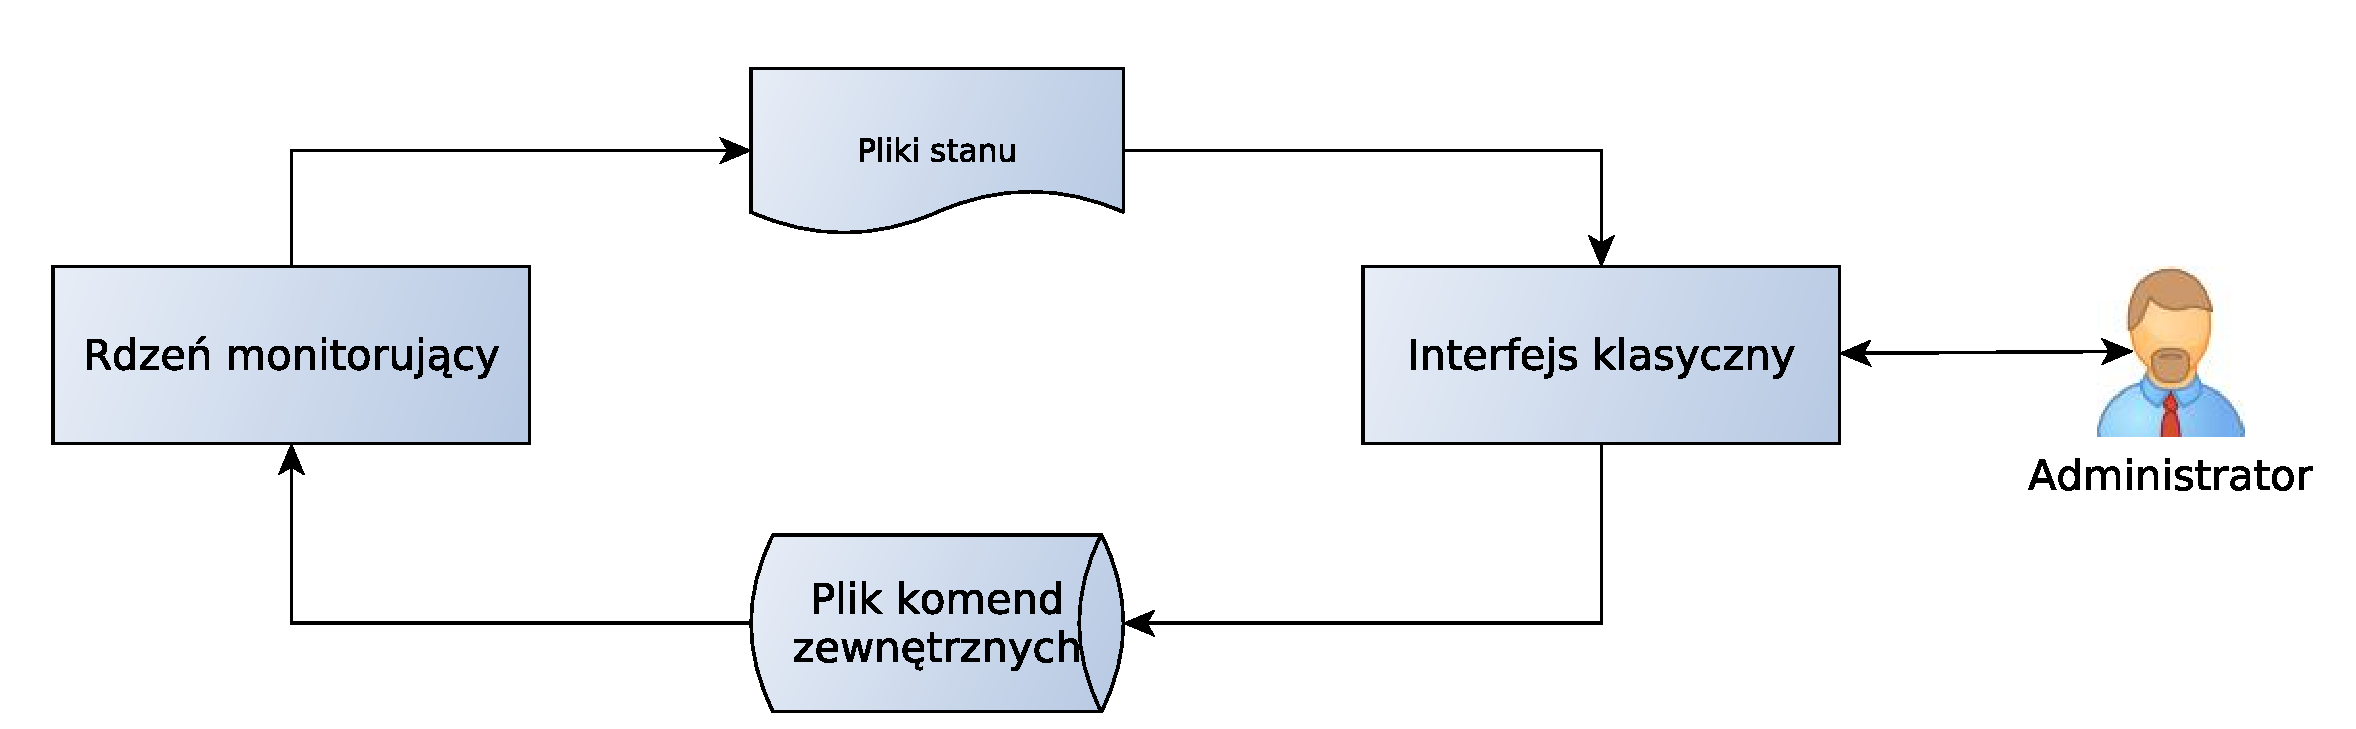
\includegraphics[width=1\textwidth]{img/icingaMini}
\end{figure}

Podstawową metodą optymalizacji przedstawionej konfiguracji jest
rozmieszczenie rdzenia monitorującego oraz interfejsu użytkownika na
różnych urządzeniach fizycznych. Umożliwienie rozdzielenia tych dwóch
bytów wymaga zapewnienia im wspólnego miejsca, w~którym składowane
będą dane konfiguracyjne, dane zawierające bieżący stan sieci oraz
reprezentację powstałych zdarzeń. System Icinga wykorzystuje do tego
celu relacyjną bazę danych. Klasyczny interfejs nie wspiera
komunikacji poprzez bazę danych, dlatego należy wykorzystać interfejs
icinga-web. Zapewnienie współpracy rdzenia monitorującego z~baza
danych odbywa się poprzez komponent IDOUtils opisany
w~\ref{sec:IDOUtils}. System składa się zatem z~następujących
elementów:

\begin{itemize}
\item rdzeń monitorujący
\item baza danych
\item interfejs graficzny
\end{itemize}

%obrazek o co kaman
Logiczny schemat konfiguracji został przedstawiony na
\ref{fig:icingaBase}. Dzięki modularnej budowie całego systemu możliwe
jest umieszczenie każdego z~wymienionych elementów na osobnym
urządzaniu fizycznym.  Umożliwia to odciążenie urządzenia, na którym
uruchomiony jest rdzeń monitorujący. Ponadto zwiększone zostaje
bezpieczeństwo całego rozwiązania, gdyż konieczne jest udostępnienie
na zewnątrz jedynie serwera na którym znajduje się interfejs
sieciowy. Urządzenie to musi mieć dostęp do bazy danych, lecz nie musi
mieć dostępu do urządzenia, na którym umieszczony jest rdzeń
monitorujący oraz do całej monitorowanej infrastruktury. Pozwala to na
umieszczenie rdzenia monitorującego razem z~monitorowaną
infrastrukturą za zaporą ogniową, co ogranicza możliwości ingerencji
w~system monitorowania i~infrastrukturę sieciową.

\begin{figure}[ht]
  \caption{Schemat podstawowej konfiguracji systemu Icinga.}
  \label{fig:icingaBase}
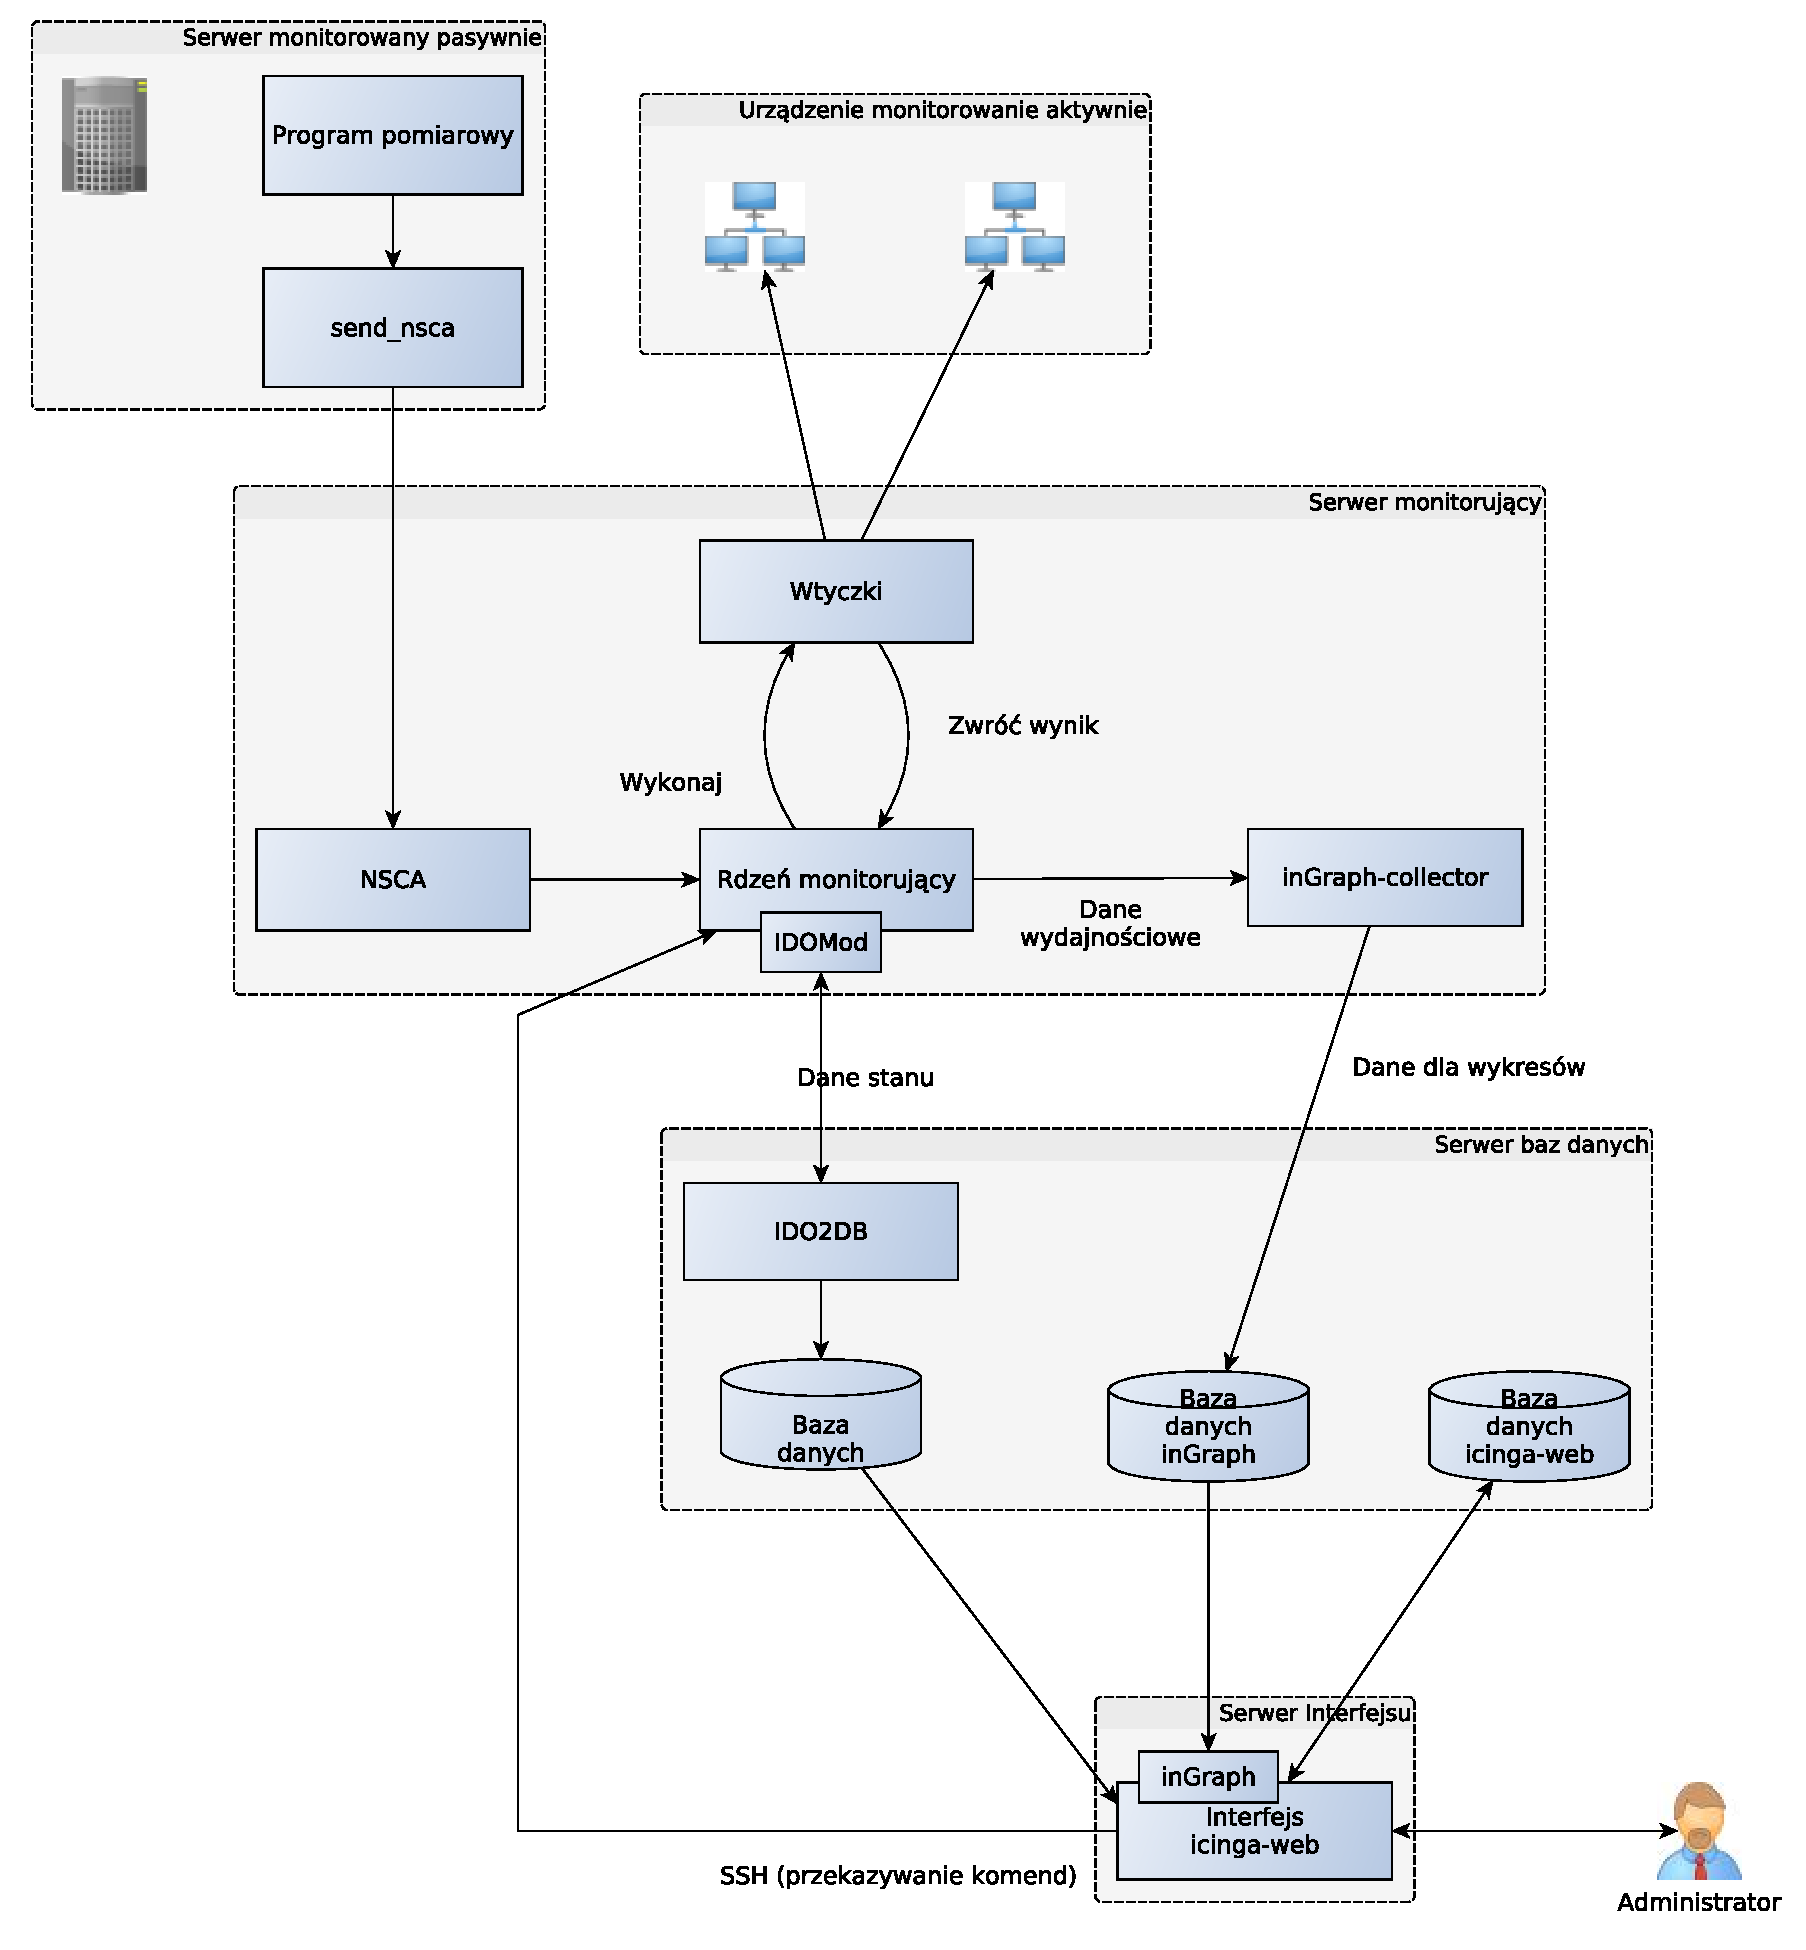
\includegraphics[width=1\textwidth]{img/icingaBase}
\end{figure}

Przedstawiona architektura stanowi bardzo dobrą konfigurację dla firm
posiadających jednolitą infrastrukturę sieciową o~średniej
wielkości. Istnieją jednak sieci dla których przedstawiona
architektura może okazać się niewystarczająca. Jedna z~takich sytuacji
ma miejsce, gdy instytucja posiada sieć złożoną z~kilku segmentów czy
to ze względu na separacje czy też lokalizacje
geograficzną. Przedstawiona architektura nie umożliwia monitorowania
aktywnego, urządzeń znajdujących się za zaporą ogniową. Możliwe jest
monitorowanie pasywne takich usług jednak wymaga ono ingerencji
w~monitorowane serwery. Kolejna z~sytuacji ma miejsce, gdy
monitorowana infrastruktura, jest na tyle rozbudowana, że urządzenie
na którym uruchomiony jest rdzeń nie posiada wystarczającej ilości
zasobów, aby monitorować wszystkie urządzenia i~usługi. Obie te
sytuacje wymagają monitorowania przy jednoczesnym użyciu wielu
instancji rdzenia monitorującego.


Pierwszy z~możliwych scenariuszy współpracy wielu instancji rdzenia
monitorującego wymaga zastosowania dodatku NSCA omówionego
w~\ref{sec:NSCA}. Konfiguracja ta zakłada istnienie jednej wyróżnionej
instancji rdzenia monitorującego, która będzie odpowiedzialna za
przetwarzanie wszystkich wyników sprawdzeń, a~także generacje zdarzeń
i~powiadomień. Konieczne jest również zapewnienie możliwości
komunikacji z~co najmniej jednego urządzenia w~każdym segmencie
sieci. Konfiguracja ta została oparta o~mechanizm pasywnego sprawdzana
usług i~urządzeń. Instancja centralna posiada wszystkie usługi
skonfigurowane w~taki sposób, aby możliwe było dostarczanie pasywnych
wyników sprawdzeń tych usług. Na tym samym systemie, co wyróżniona
instancja rdzenia uruchomiony jest również serwis systemowy NSCA,
który oczekuje na dane przesyłany z~instancji roboczych. Każda
z~instancji roboczych może zarówno wykonywać monitorowanie aktywne jak
i~pasywne pewnej części usług lub urządzeń. Wyniki sprawdzeń nie są
jednak przetwarzane przez instancję roboczą, lecz są przesyłane
z~użyciem send\_nsca do instancji centralnej, w~której następuje
odpowiednie przetwarzanie. Schemat współpracy poszczególnych elementów
systemu w tej konfiguracji zawarto na \ref{fig:rozpNSCA}.

\begin{figure}[ht]
  \caption{Schemat konfiguracji rozproszonej z~instancją centralną.}
  \label{fig:rozpNSCA}
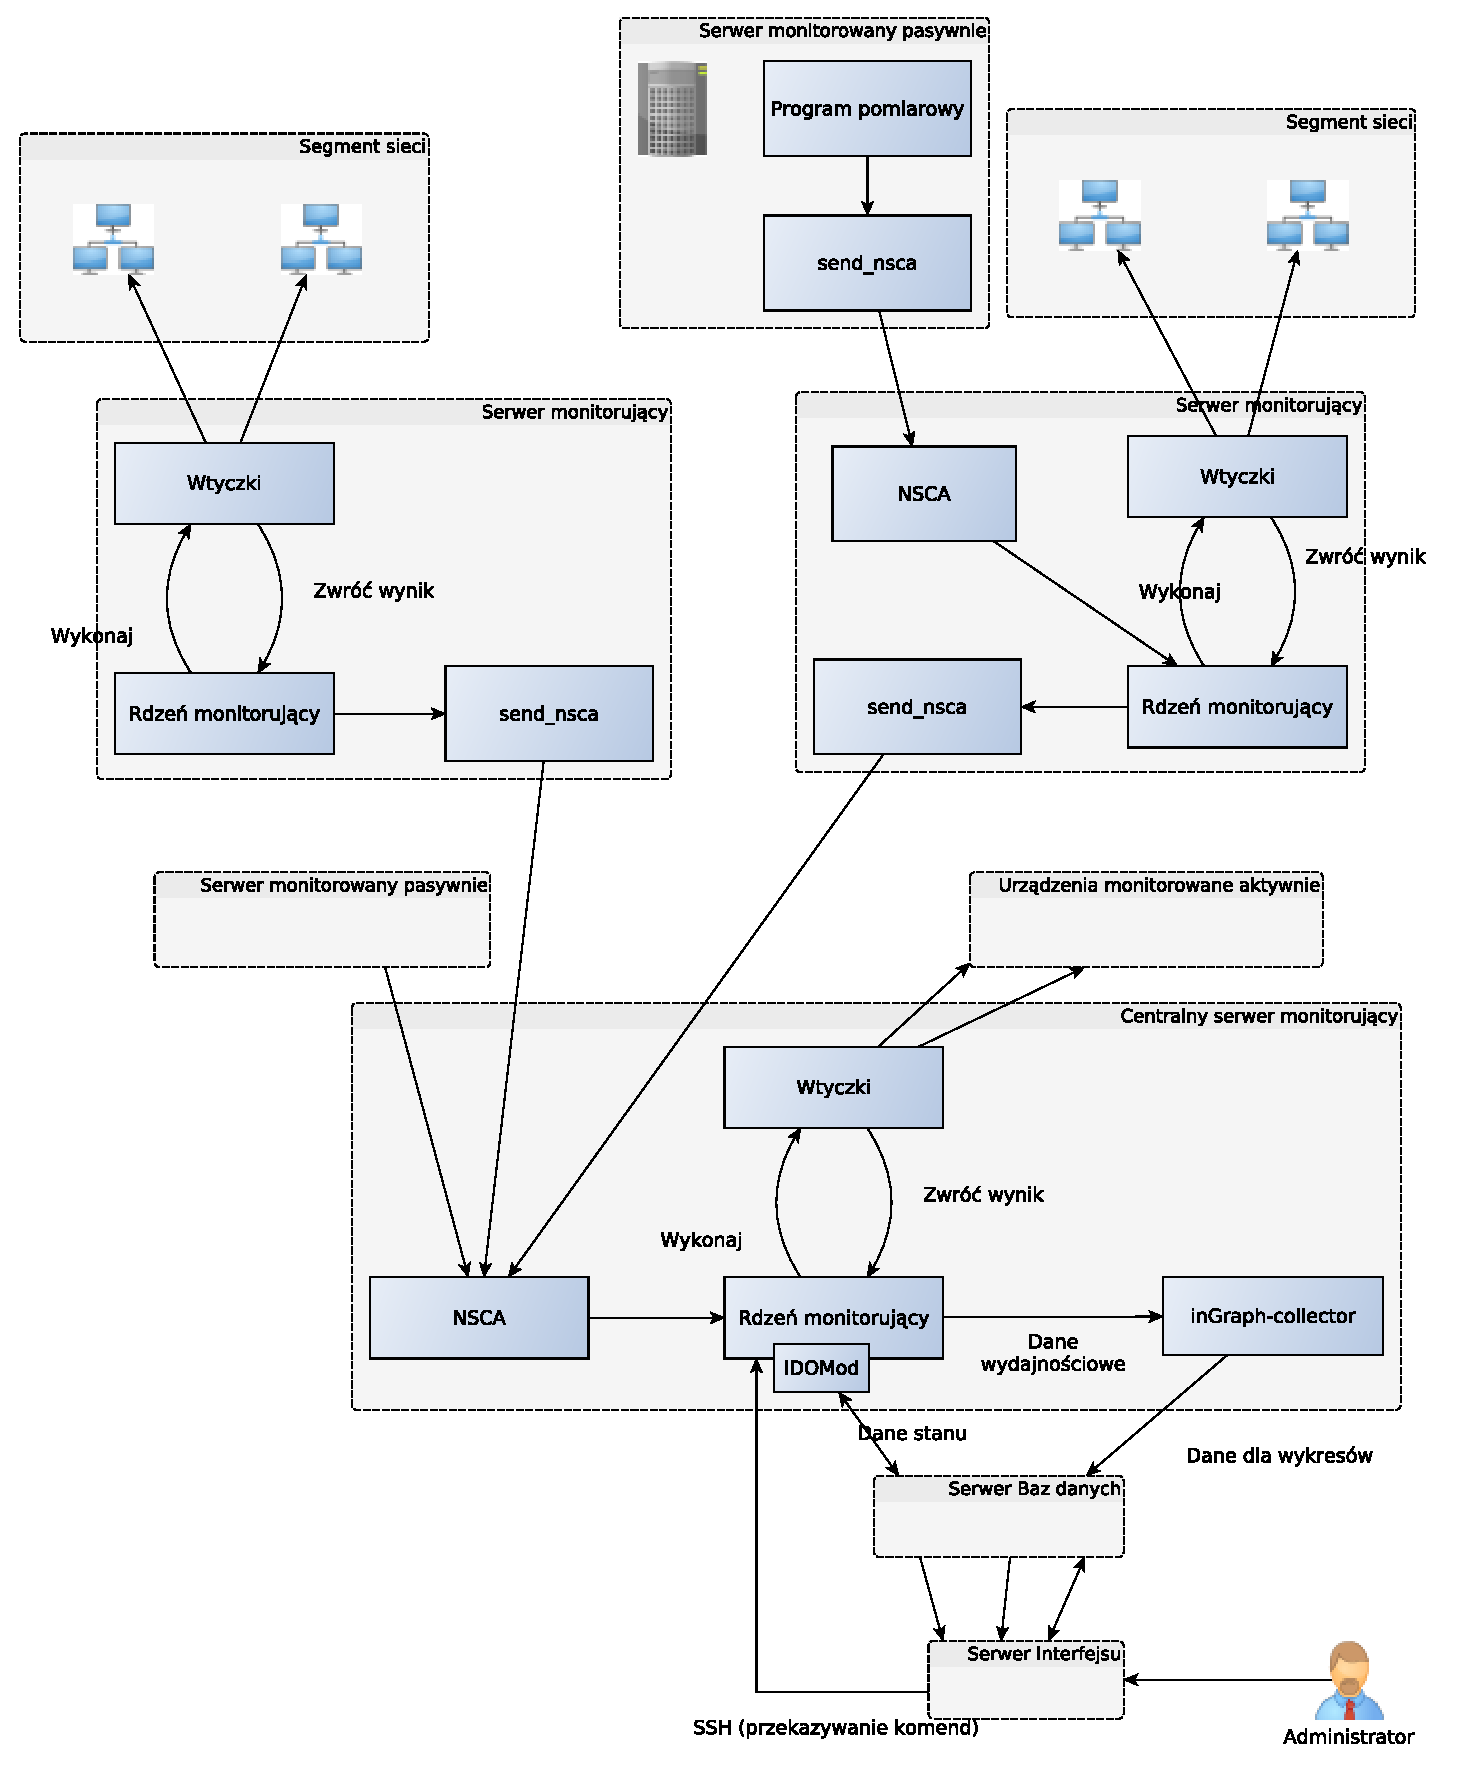
\includegraphics[width=1\textwidth]{img/icingaNSCA}
\end{figure}

Kolejnym z~możliwych scenariuszy współpracy wielu instancji rdzenia
monitorującego jest wykorzystanie wspólnej bazy danych. Rozwiązanie to
wymaga jedynie, aby wszystkie instancje rdzenia miały dostęp do jednej
bazy danych. Wszystkie instancje są w pełni niezależne i~każda z~nich
monitoruje w~dowolny sposób pewną grupę usług i~urządzeń. Wyniki
monitorowania są przetwarzane, przez każda instancję niezależnie, a~na
podstawie ich przetwarzania generowane są odpowiednie zdarzenia. Przy
użyciu komponentu IDOUtils wszystkie te dane są konsolidowane w
wspólnej bazie danych z~której korzysta interfejs icinga-web. Dzięki
wykorzystaniu nowego interfejsu możliwe jest równoczesna prezentacja
wyników monitorowania pochodzących od wielu instancji, przy użyciu
jednego interfejsu. Logiczny schemat tej konfiguracji przedstawiono na
\ref{fig:rozpFull}.

\begin{figure}[ht]
\centering
  \caption{Schemat konfiguracji rozproszonej ze~wspólną bazą danych.}
  \label{fig:rozpFull}
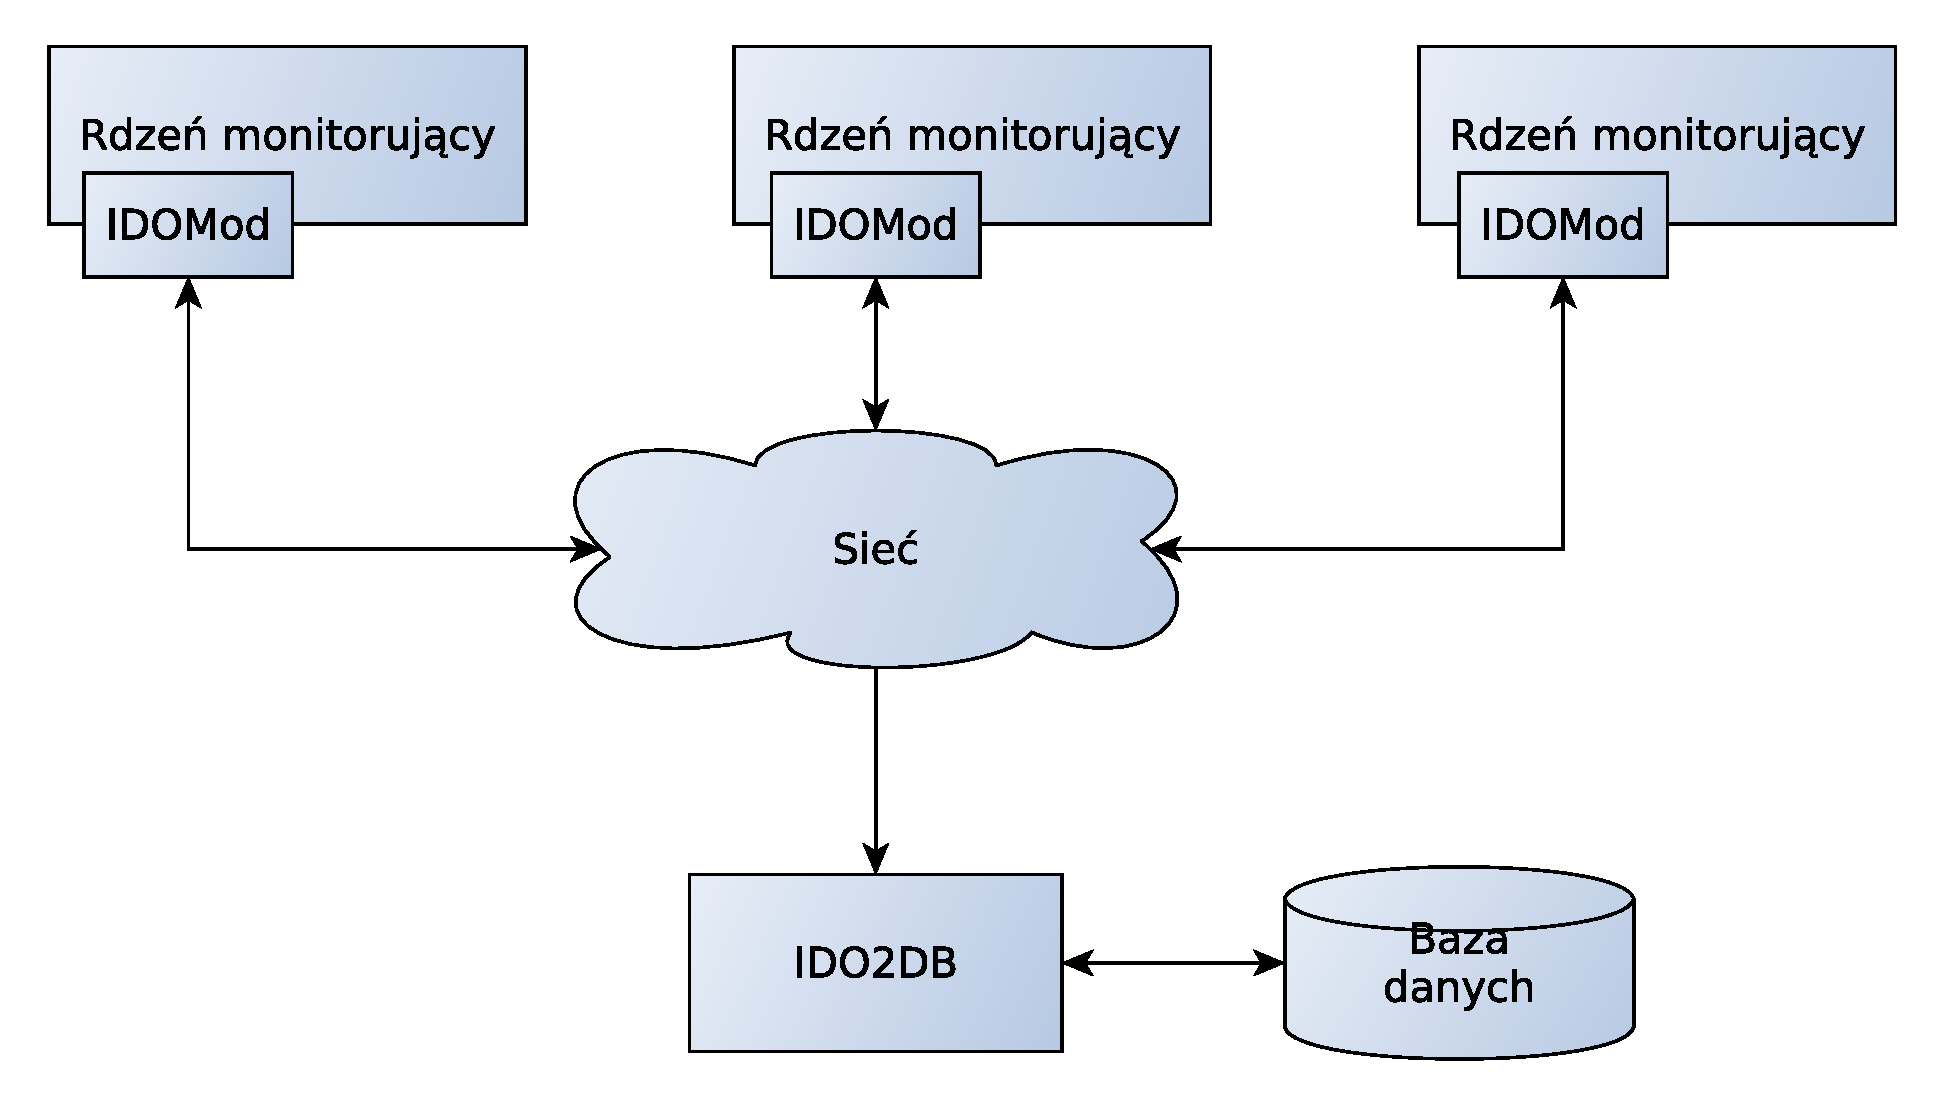
\includegraphics[width=0.8\textwidth]{img/icingaFull}
\end{figure}

Oba rozwiązania posiadają zarówno zalety jak i~wady. Rozwiązanie
z~użyciem dodatku NSCA zapewnia spójne przetwarzanie danych przez
jedna instancje i~łatwość konfiguracji dodatków wykorzystujących dane
eksportowane przez jądro w~postaci danych wydajnościowych. Niestety
rozwiązanie to generuje znaczące obciążenie instancji centralnej, gdyż
musi ona przetwarzać wszystkie wyniki sprawdzeń. Ponadto należy
przypomnieć, że model bezpieczeństwa dodatku NSCA posiada poważne
wady. Rozwiązanie oparte o~wspólną bazę danych posiada rozproszony
mechanizm przetwarzania sprawdzeń jak i~zdarzeń dzięki czemu nie
występuje w~nim nadmierne obciążenie jednej z~instancji. Ponadto
awaria, dowolnej z~instancji nie powoduje nigdy braku możliwości
monitorowania całej sieci lecz jedynie jej fragmentu. Niestety
w~rozwiązaniu tym konieczna jest bardziej zaawansowana konfiguracja
dodatków korzystających z~danych wydajnościowych. Wybór konfiguracji
zależy zatem silnie od infrastruktury w jakiej ma być ona zastosowana,
a także od pozostałych elementów systemu, jakie będą wykorzystane.


\section[Problemy][Problemy z monitorowaniem klienta mobilnego]{Problemy z monitorowaniem klienta mobilnego}

System Icinga nie posiada żadnego mechanizmu wsparcia dla klientów
mobilnych. Istnieje wiele konfiguracji rozproszonych, a~część z nich
może być zaadoptowana do monitorowania klienta mobilnego. Należy
pamiętać, iż element systemu obecny na urządzeniu mobilnym musi
oszczędzać zarówno pamięć jak i~czas procesora. Schemat logiczny
konfiguracji ze wspólną bazą danych dla klientów mobilnych został
przedstawiony na \ref{fig:mobilnyWspBaza}. Konfiguracja ta jest
niestety nieakceptowalna ze względu na konieczność przetwarzania
wszystkich informacji na urządzeniu mobilnym, co w~znaczący sposób
zwiększyłoby obciążenie klienta mobilnego.  W związku z~powyższym
zdecydowano się rozważyć konfigurację rozproszoną z~użyciem
NSCA. Wymaga ona dostarczenia elementu systemu, który będzie znajdował
się na urządzeniu mobilnym i monitorował je, a~następnie przekazywał,
gdy będzie to możliwe dane do instancji nadrzędnej, która będzie
prowadziła analizę otrzymanych danych. Schemat tej konfiguracji został
przedstawiony na \ref{fig:mobilnyInstancja}.

\begin{figure}[ht]
  \centering
  \caption{Monitoring klienta mobilnego w~konfiguracji ze~wspólną bazą
    danych.}
  \label{fig:mobilnyWspBaza}
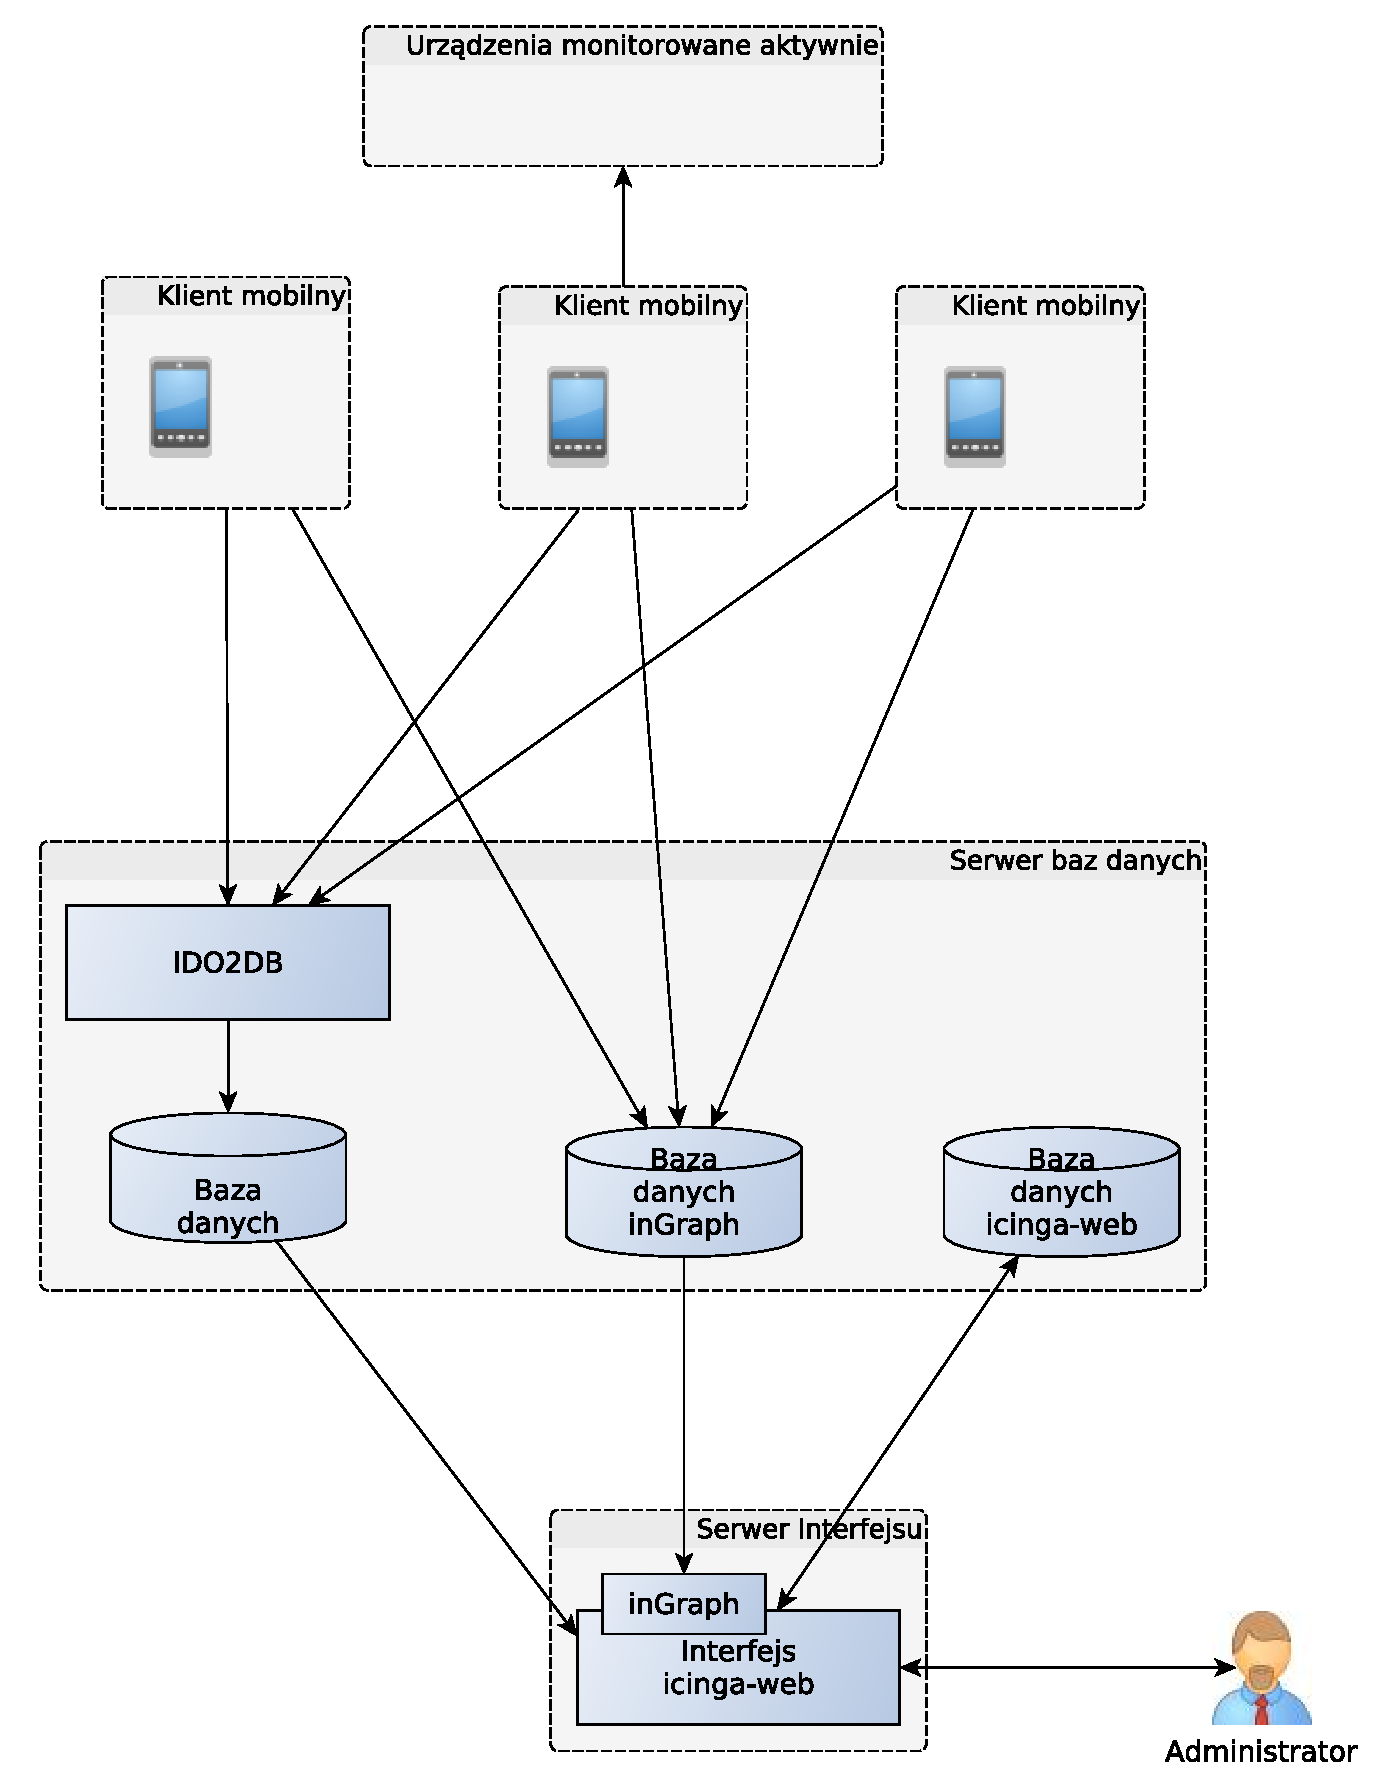
\includegraphics[width=0.75\textwidth]{img/mobilnyWspBaza}
\end{figure}

\begin{figure}[ht]
  \centering
  \caption{Monitoring klienta mobilnego w~konfiguracji z~instancją
    nadrzędną.}
  \label{fig:mobilnyInstancja}
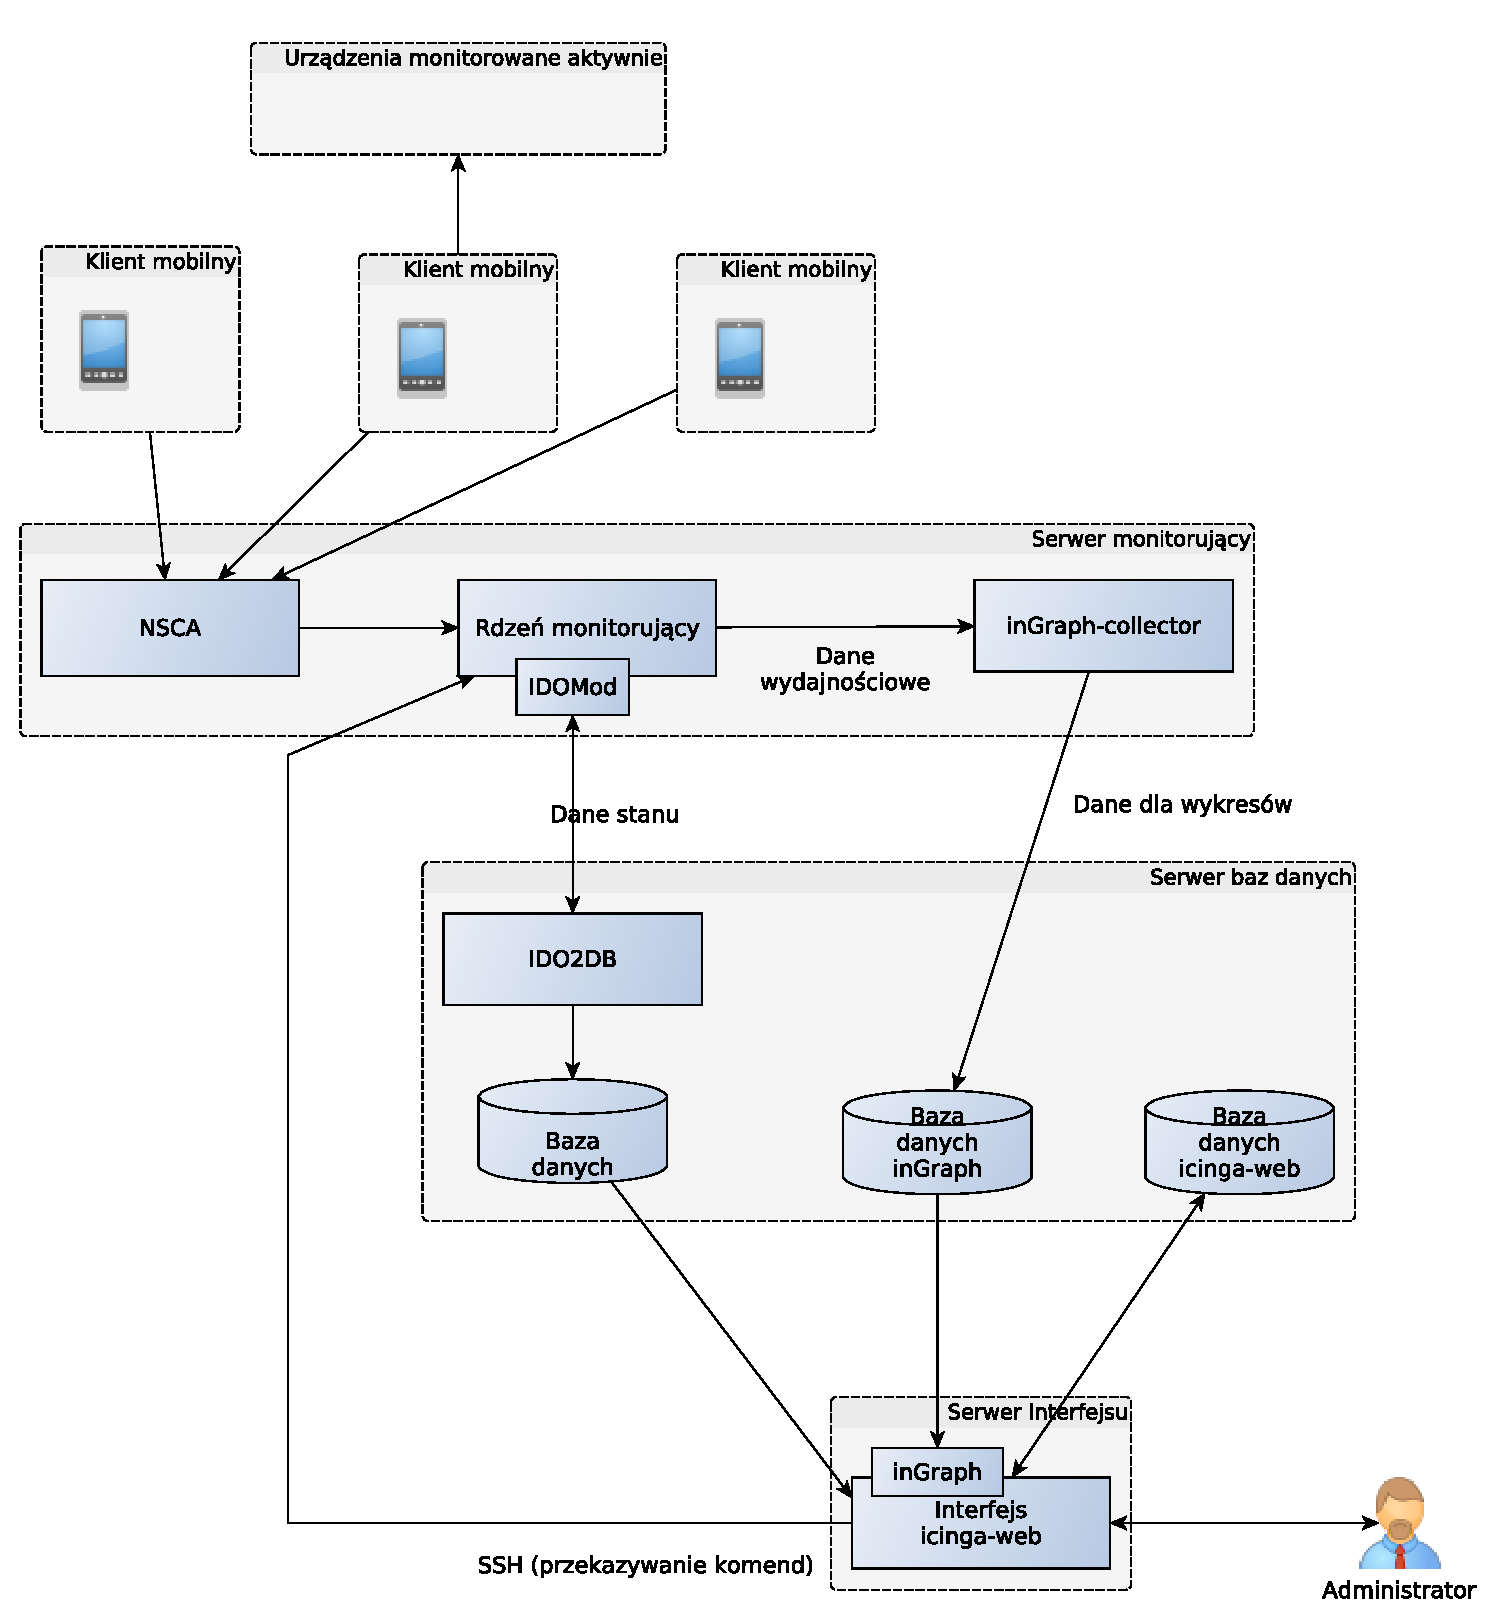
\includegraphics[width=0.80\textwidth]{img/mobilnyInstancja}
\end{figure}

Wykorzystanie do celu komunikacji pomiędzy klientem mobilnym,
a~instancja nadrzędną dodatku NSCA niesie za sobą wiele problemów.
Dodatek NSCA jest powszechnie używany do monitorowania serwerów
znajdujących się za zaporą lub w~wydzielonym segmencie sieci. Dodatek
ten może być stosowany, w~sieciach o~statycznym charakterze, gdzie
połączenia są stałe, a~łączność nie ulega częstym przerwaniom. Ponadto
należy być świadomym słabości modelu bezpieczeństwa stosowanego
w~protokole wymiany danych. Stosowanie dodatku NSCA poza zamkniętymi
sieciami firmowymi może okazać się niebezpieczne i~zawodne.

Zagadnienie monitorowania klienta mobilnego zostało szczegółowo
opisane w~\ref{chap:Wymagania}. Niestety dodatek NSCA nie spełnia
bardzo wielu z~przedstawionych wymagań przez co nie powinien być on
stosowany w~systemach tego typu. Głównymi problemami, które
dyskryminują ten w~zastosowaniu do monitorowania klienta mobilnego są:

\begin{description}
\item[Bezpieczeństwo] Mechanizmy bezpieczeństwa zawarte w~protokole
  wymiany danych posiadają poważne luki. Zastosowanie CRC32 do
  sprawdzania spójności danych niesie za sobą ryzyko ze względu na
  duże prawdopodobieństwo wystąpienia kolizji. Ponadto konieczność
  przechowywania na urządzeniu klucza symetrycznego, którego
  ujawnienie kompromituje cały system znacząco osłabia stosowane
  mechanizmy bezpieczeństwa.
\item[Nadpisywanie stempla czasu] Moduł odbierający dodaje do każdego
  wpisu dziennika aktualny stempel czasy. Powoduje to brak możliwości
  przesyłania, historycznych danych zgromadzonych w skutek utraty
  dostępu do sieci.
\item[Brak dodatkowych mechanizmów uwierzytelnienia klienta] Decyzja
  o~przydzieleniu klientowi dostępu czyli akceptacji przesłanych przez
  niego wpisów dziennika podejmowana jest na podstawie znajomości
  przez niego algorytmu szyfrowania oraz klucza.
\item[Brak kontroli otrzymywanych danych] Każdy klient, który zna
  klucz może przesyłać wpisy dotyczące dowolnego urządzenia i~dowolnej
  usługi. Brak jest mechanizmu, który pozwolił by na kontrolę tego,
  jaki klient ma prawo informować o~jakim urządzeniu czy też usłudze.
\item[Brak potwierdzenia dostarczenia danych] Klient wysyłający dane
  nie ma żadnej informacji o~tym, czy jego dane zostały zaakceptowane
  czy odrzucone. Oznacza to brak możliwości synchronizacji danych na
  kliencie mobilnym i~serwerze, gdyż nigdy nie mamy gwarancji, że
  wysłane przez klienta dane zostały przetworzone przez dodatek NSCA
  i~przekazane do rdzenia monitorującego.
\item[Brak implementacji dla systemów mobilnych] Moduł wysyłający jest
  aktualnie zaimplementowany jedynie na systemy Windows oraz
  Linux. Wiele współczesnych urządzeń mobilnych, które powinny być
  monitorowane funkcjonuje pod kontrolą systemu operacyjnego Android
  czy też Windows Phone.
\item[Przekazywanie danych tylko w~jedno miejsce] Dane odebrane przez
  moduł odbierający mogą być przekazane jedynie w~jedno miejsce. Przy
  bardziej złożonych systemach, konieczna jest możliwość przekazywania
  danych do kilku systemów oraz definiowania reguł, które dane gdzie
  powinny trafić.
\end{description}

Zastosowanie konfiguracji z~nadrzędną instancją rdzenia monitorującego
stanowi dobry szkielet dla systemu monitorowania klienta
mobilnego. Niestety dostępne na rynku narzędzie, to jest dodatek NSCA
nie są odpowiednio przystosowane do użycia ich w takim systemie. Wobec
braku dostępnych narzędzi na rynku konieczne jest zaprojektowanie oraz
zaimplementowanie nowego narzędzie, które spełni stawiane przed nim
wymagania.

%\chapter{Architektura proponowanego systemu}
\label{chap:ArchCal}

\section[Podział na moduły][Podział na moduły]{Podział na moduły}

Monitorowanie klienta mobilnego jest zagadnieniem złożonym. Niestety
nie jest możliwe zaadoptowanie bez modyfikacji żadnego z~dostępnych na
rynku systemów. Wymagania przedstawione w~\ref{chap:Wymagania}
wymuszają budowę systemu monitorowania, który będzie umożliwiał
monitorowanie zarówno klienta mobilnego jak i~statycznego. Napisanie
całości takiego systemu jest zadaniem bardzo obszernym. Warto tutaj
nadmienić, że jądro monitorujące systemu Icinga zostało napisane
w~języku~C i~zajmuje 315~000 linii kodu. Na tej podstawie uznano za
niemożliwe napisanie systemu o~funkcjonalności szerszej od
wspominanego w~ramach pracy inżynierskiej.

Kolejnym argumentem przeciw tworzeniu takiego systemu od podstaw jest
konieczność przeprowadzenia obszernych testów. Większość systemów
dostępnych na rynku posiada rozbudowany system testów autoamtycznych,
a~także szeroką społeczność, co powoduje, że kod w nich zawarty jest
dobrze przetestowany, a~jego jakoś jest bardzo wysoka.

W obec powyższych, bezsprzecznie słusznych argumentów, w~ramach tej
pracy inżynierskiej zaproponowano system monitorujący oparty
o~rozwiązania dostępne na rynku, które zostały zmodyfikowane, aby
umożliwić monitoring klienta mobilnego. Proponowany system składa się
z~trzech modułów pełniących następujące funkcje:

\begin{itemize}
\item Moduł podstawowy, odpowiedzialny za bezpośredni monitoring
  klientów statycznych oraz analizę danych od klientów mobilnych.
\item Moduł odbioru danych, odpowiedzialny za przekazywanie wpisów
  dziennika od klientów mobilnych do modułu podstawowego.
\item Moduł mobilny, odpowiedzialny za monitorowanie klientów
  mobilnych i~przekazywanie danych do modułu odbioru danych.
\end{itemize}

%dodac rysunek z tymi komponentami
%dodac referencje do wiki icingi
Elementy modułu podstawowego rozmieszczone są na serwerach sieci
lokalnej, w~której znajdują się klienty statyczne. Moduł ten zapewnia
ich monitorowanie oraz stanowi interfejs dostępowy dla
administratora. W~przedstawionej kofiguracji istnieje tylko jedna
instancja jądra monitorującego, lecz możliwa jest również konfiguracją
zawierająca kilka rdzeni systemu monitorowania. Sposób wykonania
takiej kofiguracji został omowiony w~[wiki\_icingi]. Moduł odbioru
danych umieszczony jest na urządzeniu posiadającym dostęp do sieci,
w~której pracują klienty mobilne. W~omawianej kofiguracji przyjęto, iż
klienty mobilne oraz moduł odbioru danych mają dostęp do sieci
Internet. Ponadto w~celu uproszczenia omawianej kofiguracji
i~pominięcia dodatkowych elementów, które nie są przedmiotem tej
pracy, poczyniono założenie, iż moduł odbierający dane oraz rdzeń
monitorujący modułu podstawowego znajdują się na tym samym systemie
operacyjnym. Możliwa jest jednak konfiguracja, w~której wspomniane
elementy znajdują się na różnych urządzeniach. Moduł mobilny
instalowany jest na urządzeniu mobilnym, które jest monitorowane przez
system. Jest on bezpośrednio odpowiedzialny za wykonywanie
zaplanowanych odczytów oraz przekazanie ich wyników do modułu
odbierającego. Poszczególne elementy zostały omówione w kolejnych
podrozdziałach. Moduły omawianego systemu są od siebie niezależne
i~komunikują się poprzez dobrze zdefiniowane interfejsy
i~protokoły. Możliwa jest zatem zmiana przedstawionej konfiguracji,
w~taki sposób, aby spełniała ona dodatkowe oczekiwania odbiorcy.

\section[Moduł podstawowy][Moduł podstawowy]{Moduł podstawowy}

Moduł podstawowy stanowi rdzeń całego systemu monitorowania. Moduł ten
został zbudowany wykorzystując system monitorowania Icinga. System
monitorujący Icinga został szeroko opisany
w~\ref{subsec:Icinga}. Cieszy się on uznaniem środowiska
administratorów, a~jego możliwości konfiguracji umożliwiają budowę
rozległego systemu monitorowania rozproszonego zarówno dla bardzo
dużej sieci, jak i~dla dużej liczby klientów mobilnych.

Tutaj bedzie opis tego modulu

\section[Moduł odbioru danych][Moduł odbioru danych]{Moduł odbioru danych}
\label{sec:ModOdbDanych}

Moduł ten odpowiedzialny jest za odbieranie danych od klientów
mobilnych i~przekazywanie ich do modułu podstawowego. Żaden
z~dostępnych na rynku systemów monitorowania, ani dodatek do takiego
systemu, nie spełniał wymagań stawianych przed omawianym
systemem. W~związku z~powyższym moduł odbioru doanych został
zaprojektowany oraz zaimplementowany w~ramach niniejszej
pracy. Omawiany moduł jest niezależny od pozostałych. Możliwe jest
jego użycie zarówno z~innymi klientami mobilnymi, jaki z~innym
systemem monitorującym. Należy jedynie zapewnić implementacje
protokołu komunikacyjnego po stronie klienta, oraz dostarczyć metodę,
wprowadzania danych do modułu podstawowego. Omawiany moduł
przeznaczony jest dla systemów z~rodziny Linux. Składa się on
z~samodzielnego demona systemowego, którego szczegółowa architektura
została omówiona w~\ref{chap:ArchDaemona}.

%dodac odniesienia do literatury o AES i CBC
Moduł ten spełnia kilka bardzo ważnych funkcji. Podstawowym jego
zadaniem jest odbieranie danych od klienta. Zgodnie z~wymaganiami
określonymi w~\ref{chap:Wymagania} konieczne jest, aby system
zapewniał zarówno poufność jak i~integralność danych. Oba te wymagania
są spełnione przez ten system, poprzez użycie kryptografi oraz funkcji
skrótu, które pozwalają jednoznacznie zweryfikować integralność
wiadomości. System jest niezależny od zastosowanego algorytmu
szyfrowania danych. W omawianej konfiguracji, do transportu danych
został wykorzystany algorytm AES pracujący w trybie wiązania bloków
zaszyfrowanych (CBC). Jako długość klucza przyjęto 128 bitów, pomimo,
iż jest to najmniejsza z~dostępnych długosci klucza AES jest ona
wystarczająca do tego zastosowania.

Kolejnym zadaniem omawianego modułu jest uwierzytelnienie klienta. Dla
celów demonstracyjnych dostarczono dwa moduły
uwierzytelnienia. Pierwszy z~nich to uwierzytelnienie zawsze
pozytywne, które pozwala na dostęp każdemu klientowi. Drugi natomiast,
to proste uwierzytelnienie na podstawie nazwy użytkownika oraz hasła
przydzielonego przez administratora\footnote{Przedstawione moduły mają
  charakter czysto akdemicki i~służą jedynie zaprezentowaniu
  niezalezności modułu odbierania danych od wybranej metody
  uwierzytelnienia użytkownika. Wszystkie nazwy użytkowników oraz
  hasła, używane przez jedną z~metod przechowywane są jawnym
  tekstem. Przed użyciem systemu należy skonfigurować metodę
  uwierzytelnienia urzytkownika zgodnie z polityką stosowaną w danej
  sieci.}. Możliwe jest skonfigurowanie dowolnej motody
uwierzytelnienia klienta, zgodnie z polityką bezpieczeństwa stosowaną
w~danej sieci.

Odebrane od klienta dane są przechowywane przez moduł z~wykorzystaniem
pamięci trwałej, co umożliwa bardzo szybkie potwierdzenie odebrania
danych, jeszcze przed przekazaniem ich do miejsc
przeznaczenia. Omawiany moduł, na podstawie pliku konfiguracyjnego
dostarcza dane do wskazanych miejsc docelowych. Możliwe jest
definiowanie dowolnych miejsc przeznaczenia dla danych, co umożliwia
przekazywanie danych pochodzących od klienta do wielu systemów bez
konieczności ich retransmisji. Zastosowany plik pośredni gwarantuje,
iż czas zapisu danych w~miejsce docelowe, nie będzie wydłużał czasu
oczekiwania na potwierdzenie przyjęcia danych od klienta. Warto
zauważyć również, że dane odebrane przez ten moduł zostaną zawsze
dostarczone do ich miejsc docelowych, lub jawnie usuniętę przez
administratora. Oznacza to zatem, iż moduł gwarantuje dostarczenie
danych, natomiast wykrywanie duplikatów danych jest wykonywane
w~miejsca docelowych dla danych.

%Trzeba bedzie dopisac o walidacji danych jesli faktycznie bedzie tutaj robiona

\section[Moduł mobilny][Moduł mobilny]{Moduł mobilny}

Moduł ten jest odpowiedzialny za monitorowanie zadanych parametrów
urządzenia mobilnego. Każdy klient mobilny posiada swoją instancję
tego modułu, która jest odpowiedzialna za monitorowanie jego
urządzenia. Ten elemento systemu powinien posiadać budową
modularną. Najważniejsze z wymagań odnoszocych się do tego modułu
wymusza, aby możliwe było w jak najprostszy sposób dodawanie
możliwości sprawdzania nowych parametrów.  

Ponad to implementacja tego modułu musi brać pod uwagę architekturę
sprzętową na której pracuje. Urządzenia mobilne są zazwyczaj zasilane
z~własnych akumulatorów dlatego konieczne jest zastosowanie
mechanizmów, które pozwolą na zredukowanie zużycia energii związanego
z~systematycznym wykonywaniem sprawdzeń. Należy równiez wspomnieć, iż
moduł mobilny odpowiedzialny jest za nadawianie każdemu z~odczytów
stempla czasu uniwersalnego dokonywanego pomiaru. Na podstawie
dokonanej charakterystyki klienta mobilnego, w~niniejszej pracy
poczyniono założenie, iż klient posiada dostęp do punktów
synchronizacji czasu. Jest wiele dostępnych metod synchronizacji czasu
na urządzeniu mobilnym, midzy innymi pobranie czasu z~sieci GSM czy
też z~serwerów czasu światowego, przez co nie stanowi to dla klienta
mobilnego poważnego wymagania.

Klient mobilny po zebraniu porcji wpisów dziennika o~rozmiarze zgodnym
z~polityką administratora, lub po upływie określonego czasu powinien
przesłać posiadane wpisy dziennika do modułu odbiorczego, a~po
uzyskaniu potwierdzenia usunąć je z~urządzenia w~celu oszczędności
pamięci. Różnorodność platform dostępnych na rynku sprawia, iż nie
jest możliwe dostarczenie uniwersalnej implementacji protokołu
komunikacyjnego dla wszystkich platform mobilnych. Oznacza to, iż
przed klientem mobilnym stawia się wymóg zarówno implementacji
protokołu komunikacyjnego jak i~odpowiednich mechanizmów
uwierzytelnienia klienta. Protokół komunikacyjny został szczegółowo
opisany w~\ref{chap:ProtKom}.

%dodać referencje do pracy kubika
W ramach omawianego systemu wykorzystano wiele instancji modułu
mobilnego zaprojektowanego i~zaimplementowanego przez Pana Marcina
Kubika. Moduł ten został szeroko omówiony w [praca\_kubika]. Całość
systemu jest niezależna od platformy klienta mobilnego, zatem mozliwa
jest współpraca całości systemu z~klientami mobilnymi przeznaczonymi
dla innych platform, jednak muszą one implementować protokół
komunikacyjny wykorzystywany przez moduł pośredniczący.

%\chapter{Monitorowanie rozproszone z użyciem NSCA}
\label{chap:nsca}

\section[Opis dodatku NSCA][Opis dodatku NSCA]{Opis dodatku NSCA}

NSCA - Nagios Service Check Acceptor jest to dodatek do systemów
monitorujących opartych o~system Nagios, więc również systemu
Icinga. Pozwala on na wykorzystanie mechanizmów pasywnego
monitorowania z~systemu innego niż ten na którym uruchomione jest
oprogramowanie monitorujące. Program ten został napisany w całości w
języku~C i~wydany na licencji pozwalającej na wgląd do kodu
źródłowego. Wykorzystuje on plik zewnętrznych komend i nie integruje
się z jądrem monitorującym. Dzięki temu możliwe jest jego
wykorzystanie zarówno w systemie Nagios jak i jego klonach takich jak
system Icinga. Dodatek ten składa się z~dwóch modułów:

\begin{itemize}
\item moduł wysyłający (send\_nsca) służący do wysyłania wyników
  sprawdzeń z~monitorującego systemu do centralnego serwera, na którym
  umieszczony jest rdzeń systemu monitorującego odpowiedzialny za
  przetwarzanie wyników sprawdzeń,
\item moduł odbierający (nsca) służący do odbierania wyników sprawdzeń
  od klientów i~dostarczaniu ich do pliku komend zewnętrznych danego
  systemu monitorującego.
\end{itemize}

%tutaj wstawic grafike z tym jak to dziala
%źrodło: dokumentacja w repo

\subsection[Moduł wysyłający][Moduł wysyłający]{Moduł wysyłający}
\label{subsec:modulWysylajacy}

Ta część dodatku uruchamiana jest na systemie, na którym funkcjonuje
jakiś mechanizm sprawdzający, który generuje wpisy dziennika. Wpisy te
po utworzeniu, przekazywane są do programu wysyłającego. Moduł
wysyłający, po uruchomieniu odczytuje ustawienia z pliku
konfiguracyjnego, a następnie próbuje połączyć się z serwerem. Po udej próbie
połączenia otrzymuje pakiet inicjujący, który zawiera:

\begin{itemize}
\item wektor inicjalizacyjny: używany do celów kryptogrficznych,
  wygenerowany przez serwer pseudolosowy ciąg znaków, konieczny do
  inicjalizacji algorytmu kryptograficznego,
\item stempel czasu: czas odczytany przez serwer w~chwili nadejścia
  połączenia od klienta.
\end{itemize} 

Po otrzymaniu pakietu inicjującego moduł rozpoczyna czytanie wpisów z
standardowego wejścia programu. Wszystkie wpisy dziennika muszą być odpowiednio
sformatowane. Poszczególne pola informacyjne muszą być rozdzielone
pojedyńczą tablulacją, a~cały wpis zakończony znakiem nowej
linii. Wpisy dotyczącego urządzenia powinny zawierać następujące pola:

\begin{itemize}
\item nazwa urządzenia: krótka nazwa urządzenia, którego stan jest
  przekazywany,
\item stan: numerycznie wyrażony kod stanu urządzenia,
\item odczyt: dodatkowe wartości odczytów opisujące stan urządzenia.
\end{itemize}

Natomast wpisy dotyczące usługi świadczonej przez to urządzenia, lub
innego rejestrowanego paramatru tego urządzenia powinny zawierać
następujące pola:

\begin{itemize}
\item nazwa urządzenia: krótka nazwa urządzenia na którym uruchomiona
  jest usługa,
\item opis usługi: nazwa usługi danego urządzenia, której dotyczy wpis
\item stan: numerycznie wyrażony kod stanu usługi,
\item odczyt: dodatkowe wartości odczytów opisujące stan usługi.
\end{itemize}

%dodac odniesienie do odpowiedniego rozdzialu
Łatwo zauważyć, że żadne z pól wpisu w dzienniku nie zawera stempla
czasu wymaganego przez jądro sprwdzające przy zapamiętywaniu odczytu
pasywnego. Dzieje się tak, gdyż program NSCA posiada zdefiniowaną
własną politykę określania czasu wpisu w dzienniku. Do każdego pakietu
zawierającego wpis dziennika dodawany jest stempel czasu otrzymany w
pakiecie inicjującym od modułu odbierającego. Właściwy stepel czasu,
który trafia do jadra sprawdzającego nadawany jest natomiast przez
moduł odbierający.

Kolejnym krokiem działania modułu jest obliczenie cyklicznego kodu
nadmiarowego CRC32 dla danego pakietu. Po dołączeniu obliczonego kodu
do pakietu pakiet jest szyfrowany. Algorytm szyfrujący stosowany do
szyfrowania pakietów został wcześniej zainicjalizowany wektorem
pseudolosowych danych odebranych w pakiecie inicjalizacyjnym od modułu
odbierającego. Po zaszyfrowaniu dane są wysyłane, a moduł wysyłający,
bez oczekiwania na potwierdzenie przetworzenia przez serwer,
rozpoczyna przetwarzanie kolejnego wpisu dziennika.

\subsection[Moduł odbierający][Moduł odbierający]{Moduł odbierający}

Demon, który stanowi moduł odbierający funkcjonuje na tym samym
systemie operacyjny na którym znajduje się jądro systemu
monitorującego. Ta część odpowiedzialna jest za odbieranie danych od
klientów i przekazywanie ich do jądra programu monitorującego. Moduł
ten może pracować w jednym z poniższych trybów:

\begin{itemize}
\item samodzielny demon jednoprocesowy: uruchomiony w tle demon, który
  nasłuchuje na przychodzące połączenia od klientów i po nadejściu
  połączenia jest ono obsługiwane przy użyciu jednego procesu z jednym
  wątkiem,
\item samodzielny demon wieloprocesowy: uruchomiony w tle demon,
  którego proces główny nasłuchuje na nadejście połączeń od klientów,
  gdy takie połączenie nadejdzie proces jest duplikowany i każdy z
  klientów obsługiwany jest w innym procesie potomnym,
\item demon zintegrowany z inetd: w systemie uruchomiony jest demon
  inetd, który nasłuchuje na połączenia od klientów na konkrentym
  gnieździe, a gdy nadejdzie połączenie od klienta uruchamiany jest
  proces demona NSCA, który obsługuje nowe połączenie i kończy się
  wraz z zakończeniem obsługi klienta
\end{itemize}

Do przekazywania wpisów dziennika używany jest mechanizm pasywnego
monitorowania dostępny w systemach z rodziny Nagios. Aby możliwe było
wykorzysanie tego mechanizmu konieczne jest zapewnienie demonowi
dostępu do pliku zewnętrznych komend systemu monitorującego. Ponieważ
plik zewnętrznych komend jest potokiem nazwanym, chroniony jest on
przez Uniksowy system uprawnień użytkowników. Zapewnienie dostępu do
takiego bytu może się odbyć na dwa sposoby. Pierwszym, polecanym przez
twórców systemów monitorujących, jest uruchamianie demona NSCA jako
procesu tego samego użytkownika co proces jądra systemu
monitorującego. Drugim sposobem jest modyfikacja praw dostępu do
omawianego pliku, tak aby umożliwić dostęp użytkownikowi z którego
uprawnieniami uruchomiony jest demon NSCA. Przy zastosowaniu drugiego
rozwiązania zalecana jest szczególna ostrożność, gdyż dostęp do pliku
zewnętrznych komend daje bardzo duże możliwości ingerencji w system
monitorujący.

Komunikacja modułu odbirającego z~klientem rozpoczyna się od nadejścia
połączenia od klienta. Gdy moduł odbierający otrzyma nowe połączenie
zostanie wysłany pakiet inicjalizujący, którego zawartość została
opisana w~\ref{subsec:modulWysylajacy}. Po przesłaniu pakietu
inicjalizującego połączenie, moduł odbierający oczekuje na dane od
klienta. Każdy wpis dziennika przesyłany jest przy użyciu pakietu
o~poniższych polach:

\begin{itemize}
\item wersja protokołu: aktualnie używana wersja protokołu komunikacyjnego,
\item kod CRC32: kod CRC32 bieżącego pakietu,
\item stempel czasu: stempel czasu pochodzący z~pakietu
  inicjalizującego przesłanego klientowi,
\item kod statusu: kod stanu usługi/hosta powiązany z~przesyłanym wpisem
\item nazwa hosta: nazwa klienta, który podlegał sprawdzeniu. Nie jest
  konieczne aby był to ten sam klient, który dostarcza dane,
\item opis usługi: nazwa usługi, która podlegała sprawdzeniu lub pusty
  napis jeśli sprawdzenie dotyczy hosta,
\item wynik sprawdzenia: napis wygenerowany przez wtyczkę, która
  dokonywała sprawdzenia, zawierajacy dodatkowe dane na temat stanu
  urządzenia lub usługi
\end{itemize}

Pakiety są zaszyfrowane z~użyciem algorytmu oraz klucza symetrycznego
pochodzącego z~pliku konfiguracyjnego. Po odebraniu spodziewanej
ilości danych, następuje próba odszyfrowania odebranych
danych. Sprawdzenie poprawności odebranych danych i~jednocześnie
weryfikacja uprawnień odbywa się poprzez kontrolę zawartości pola
CRC32. Jeśli wartość znajdująca sie w~tym polu, zgadza się z wartością
wyliczoną dla całości otrzymanych danych, to pakiet jest przyjmowany,
w~przeciwnym zaś razie pakiet zostanie odrzucony. Dalsze przetwarzanie
otrzymanego pakietu rozpoczyna się od porównania bierzącego stempla
czasu z~tym pochodzącym z odebranego pakietu. Jeśli różnica pomiędzy
nini jest zbyt duża, dane zostają odrzucone. Ostatnią czynnością
wykonywaną przez moduł odbierajacy jest zapisanie odebranego wpisu do
pliku zewnętrznych komend jądra systemu monitorującego.

Warto wspomnieć, że stempel czasu przesłany przez klienta nie jest
dostarczany do jądra monitorujacego. Służy on jedynie określeniu
odstępu czasu od inicjalizacji sesji do chwili otrzymania wiadomości~i
podjęciu decyzji o~przyjęciu, bądź odrzuceniu pakietu. Do systemu
monitorującego trafia natomiast bierzący stempel czasu serwera, na
którym uruchomiony jest moduł odbierajacy i~jądro systemu
monitorujacego. Do generacji stempla czasu wykorzystywany jest czas
uniwersalny. Istotną, może się również okazać informacja, iż protokół
komunikacyjny nie przewiduje przesyłania ACK\footnote {ang. {\em
    Acknowledgement} -- pozytywne potwierdzenie, powszechnie przyjęta
  nazwa komunikatu potwierdzającego przyjęcie i przetworzenie danych
  przez aplikację}, bądź też NACK\footnote{ang. {\em
    Negative-acknowledgement} -- potwierdzenie negatywne, powszechnie
  przyjęta nazwa komunikatu oznaczająca odmowę przyjęcia lub
  przetworzenia odebranych danych}. Moduł wysyłający, ma zatem
pewność, iż wysłane przez nie go dane zostaną dostarczone, gdyż
używany jest protokół TCP, lecz nie ma żadnej gwarancji ani
informacji, że dane przesłane do modułu odbierającego zostaną
dostarczone do rdzenia systemu monitorującego.

\section[Bezpieczeństwo][Bezpieczeństwo]{Bezpieczeństwo}

%bibliografia dodac libmcrypt
Bezpieczeństwo monitorowania z~użyciem dodatku NSCA opiera się na
kryptografii symetrycznej oraz cyklicznym kodzie nadmiarowym
CRC32. Wiadomość inicjująca połączenie jest nieszyfrowana. Natomiast
każda wiadomość zawierająca wpisy dziennika jest zaszyfrowana
algorytmem wybranym podczas konfiguracji systemu. Dodatek NSCA
korzysta z~biblioteki libmcrypt i~umożliwia użycie jednego spośród
wielu algorytmów kryptografii symetrycznej, które zostały w niej
zaimplementowane. Użytkownik posiada jedynie możliwość wyboru
stosowanego algorytmu, natomiast jako tryb pracy stosowany jest tryb
sprzężenia zwrotnego szyfrogramu. Tryb ten wymaga zawsze inicjalizacji
zarówno kodera jak i~dekodera tym samym wektorem początkowym, który
w~przypadku tego protokołu, jest przesyłany przez serwer w pakiecie
inicjującym.

Wszystkie algorytmy symetryczne do prawidłowego działania wymagają,
aby komunikujące się strowny współdzieliły pewien sekret jakim jest
klucz używany do szyfrowania. Ujawnienie klucza symetrycznego wiąże
się z~kompromitacją całego systemu kryptograficznego. W dodadktu NSCA
klucz ten uzyskiwany jest z~hasła, które musi być zapisane przez
administratora systemu zarówno w części odbierającej jak
i~wysyłającej. Oczywistym jest, iż poza współdzieleniem klucza,
wszystkie komunikujące się węzły muszą używać tego samego algorytmu
kryptograficznego.

%zrodlo z kodem crc32
Algorytmy szyfrowania zapewniają tajność przesyłanej wiadomości,
jednak w~przypadku systemu monitorowania potrzebne jest również
zapewnienie integralności wiadomości. Integralność w~dodatku NSCA
zapewniana jest poprzez cykliczny kod nadmiarowy CRC32. Obliczanie
kodu CRC32 odbywa się poprzez dzielenie przesyłanego ciągu bitów przez
dzielnik o~długości 33 bitów, co daje kod CRC o~długości 32
bitów. W~celu sprawdzenia integralności, otrzymane bity są dzielone
przez kod CRC. Jeśli reszta z~dzielenia jest zero, oznacza to poprawna
weryfikację integralności wiadomości. Jeśli reszta z dzielenia jest
niezerowa oznacza to naruszenie integralności przesłanej wiadomości. W
szczególności, taka sytuacja może się zdarzyć, gdy klient używa innego
algorytmu kryptograficznego lub klucza. Pakiety, których integralność
nie zostanie pozytywanie zweryfikowana są odrzucane.

%zrodło o zagrozeniach z kodu CRC32
%stack overflow crc32 colision
Model bezpieczeństwa zastosowany w~dodatku NSCA ma bardzo wiele wad. Najwięszą
z~nich jest zastosowanie kodu CRC32 do sprawdzania integralności
przesyłanych wiadomości. Kod ten można bardzo prosto i~szybko
obliczyć, a~ponadto posiada on niewielką długość. Niestety jest on
bardzo podatny na kolizje przez co nie powinien on być stosowany
w~kryptogrfii. Prawdopodobieństwo nie znalezienia kolizji po 200~000
prób wynosi poniżej~1\%. Oznacza to iż jedynie w niespełna 1\%
przypadków koniecne będzie obliczenie więcej niż 200~000 kodów CRC
przed znalezieniem kolizji. Prawdopodobieństwo nie znalezienia kolizji
w~zalezności od liczby obliczonych kodów CRC32 przedstawiono
w~\ref{tab:CRC32Colisions}. Łatwość odnalezienia kolizji nie jest
jedyną wadą modelu bezpieczeństwa zastosowanego w dodatku NSCA. Warto
przypomnieć, iż wszystkie ustawienia zarówno modułu wysyłającego jak
i~odbierającego przechowywane są w plikach na dyskach odpowiednich
urządzeń. Pliki te zawierają również klucze symetryczne, które są
stosowane w całym systemie. Oznacza to iż uzyskanie dostępu typu
odczyt do takiego pliku powoduje utratę tajności danych przesyłanych w
całym systemie. Ponadto przyjęty model bezpieczeństwa, nie zawiera
żadnej weryfikacji danych pochodzących od klientów. Oznacza to, że
każdy klient moze przesłać wpisy dziennka, udające wpisy pochodzące od
zupełnie innych klientów. W~szczególności jeśli atakujący uzyska klucz
symetryczny, to nie tylko będzie mógł odczytywać informacje o wpisach
przesyłanych od klientów, lecz także podszywać się pod klientów
i~przesyłać fałszywe wpisy. Taka luka może być wykorzystana przy ataku
na jakąś usługę lub urządzenie. Atakujący rozpoczyna atak, po czym przechwytuje
pakiety z~wpisami dziennika, które mogą świadczyć o~rozpoczęciu
ataku i~w~zamian przesyła do serwera fałszywe pakiety informujące iż
wszystkie usługi pracują normalnie.

\begin{table}
\centering
\caption{Prawdopodopieństwo nie znalezienia kolizji w zależności od
  liczby obliczonych kodów CRC32}
\label{tab:CRC32Colisions}
\begin{tabular}{|c|c|}
\hline
Liczba obliczeń & Prawdopodobieństwo \\
\hline
50~000 & 74,7\% \\
\hline
77~000 & 50,1\% \\
\hline
78~000 & 49,2\% \\
\hline
102~000 & 29,8\% \\
\hline
110~000 & 24,5\% \\
\hline
128~000 & 14,8\% \\
\hline
150~000 & 7,3\% \\
\hline
200~000 & 0,95\% \\
\hline
\end{tabular}
\end{table} 

\section[Problemy][Problemy z monitorowaniem klienta mobilnego]{Problemy z monitorowaniem klienta mobilnego}

Dodatek NSCA jest powszechnie używany do monitorowania serwerów
znajdujących się za zaporą, która uniemożliwia wykonywanie aktywnych
sprawdzeń lub gdy charakterystyka monitorowanego parametru nie jest
przystająca do cyklicznego odpytywania. Dodatek ten może być
stosowany, w~sieciach o~statycznym charakterze, gdzie połączenia są
stałe, a~łączność nie ulega częstym przerwaniom. Ponadto należy być
świadomym słabości modelu bezpieczeństwa stosowanego w protokole wymiany
danych. Stosowanie dodatku NSCA poza zamkniętymi sieciami firmowymi
może okazać się niebezpieczne i~zawodne.

Zagadnienie monitorowania klienta mobilnego zostało szczegółowo opisane
w~\ref{chap:Wymagania}. Niestety dodatek NSCA nie spełnia bardzo wielu
z~przedstawionych wymagań przez co nie powinien być on stosowany
w~systemach tego typu. Głównymi problemami, które dyskryminują dodatek
NSCA w zastosowaniach do monitorowania klienta mbilnego są:

\begin{itemize}
\item Bezpieczeństwo: mechanizmy bezpieczeństwa zawarte w~protokole
  wymiany dancyh posiadają bardzo poważne luki. Zastosowanie CRC32 do
  sprawdzania spójności dancyh niesie za sobą bardzo duże
  ryzyko. Ponadto konieczność przechowywania na urządzeniu klucza
  symetrycznego, którego ujawnienie kompromituje cały system znacząco osłaba
  stosowane mechanizmy bezpieczeństwa.
\item Nadpisywanie stempla czasu: Moduł odbierający dodaje do każdego
  wpisu dziennika aktualny stempel czasy. Powoduje to brak możliwości
  przesyłania, historycznych danych zgromadzonych w skutek utraty
  dostępu do sieci.
\item Brak dodatkowych mechanizmów uwierzytelnienia klienta: decyzja
  o~przydzieleniu klientowi dostępu czyli akceptacji przesłanych przez
  niego wpisów dziennika podejmowana jest na podstawie znajomości
  przez niego algorytmu szyfrowania oraz klucza.
\item Brak kontroli otrzymywanych danych: każdy klient, który zna
  klucz może przesyłać wpisy dotyczące dowolnego urządzenia i~dowolnej
  usługi. Brak jest mechanizmu, który pozwolił by na kontrolę tego,
  jaki klient ma prawo informować o~jakim urządzeniu czy też usłudze.
\item Brak potwierdzenia dostarczenia danych: klient wysyłający dane
  nie ma żadnej informacji o~tym, czy jego dane zostały zaakceptowane
  czy odrzucone. Oznacza to brak możliwości synchronizacji danych na
  kliencie mobilnym i serwerze, gdyż nigdy nie mamy gwarancji, że
  wysłane przez klienta dane zostały przetworzone przez dodatek NSCA
  i~przekazane do rdzenia monitorującego.
\item Brak implementacji dla systemów mobilnych: moduł wysyłający jest
  aktualnie zaimplementowany jedynie na systemy Windows oraz
  Linux. Wiele współczesnych urządzeń mobilnych, które powinny być
  monitorowane funkcjonuje pod kontrolą systemu operacyjnego Android
  czy też Windows Phone.
\item Przekazywanie danych tylko w~jedno miejsce: dane odebrane przez
  moduł odbierający mogą być przekazane jedynie w~jedno miejsce. Przy
  bardziej złożonych systemach, konieczna jest możliwość przekazywania
  dancyh do kilku systemów oraz definiowania reguł, które dane gdzie
  powinny trafić.
\end{itemize}

Powyższe wady zdecydowanie dyskryminują dodatek NSCA jako narzędzie do
monitoringu klienta mobilnego. W~związku z~powyższym w tej pracy
zaproponowano nowy protokół komunikacyjny, który został opisany
w~\ref{chap:ProtKom} oraz dodatek do systemów z rodziny Nagios, który
implementuje ten protokół i umożliwia przekazywanie danych od klientów
mobilnych. Dokładny opis modułu odbierającego dane znajduje sie w
\ref{chap:ArchDaemona}. Moduł mobilny, z od którego dane otrzymuje
wspominany program, został zaprojektowany i zaimplementowany dla
platformy Android przez Pana Marcina Kubika, a jego opis znajduje się
w [praca\_kubika].

%\chapter{Architektura modułu odbioru danych}

\section[Podział na moduły][Podział na moduły]{Podział na moduły}

\section[Szkielet programu][Szkielet programu]{Szkielet programu}

\section[Moduł kryptograficzny][Moduł kryptograficzny]{Moduł kryptograficzny}

\section[Moduł autoryzacyjny][Moduł autoryzacji klienta]{Moduł autoryzacji klienta}

\section[Moduł TCP][Moduł komunikacji z wykorzystaniem TCP]{Moduł komunikacji z wykorzystaniem TCP}

\section[Moduł pisarza potoku][Moduł pisarza potoku]{Moduł pisarza potoku}

\section[Moduł logowania][Moduł logowania]{Moduł logowania}

%\chapter{Protokół komunikacyjny}
\label{chap:ProtKom}

\section[Podział na warstwy][Podział na warstwy]{Podział na warstwy}

\section[Warstwa formowania wiadomości][Warstwa formowania wiadomości]{Warstwa formowania wiadomości}

\section[Warstwa kryptograficzna][Warstwa kryptograficzna]{Warstwa kryptograficzna}

\section[Warstwa integralności][Warstwa integralności danych]{Warstwa integralności danych}

\section[Warstwa transportu logów][Warstwa transportu logów]{Warstwa transportu logów}






\chapter{Projekt systemu}
\label{chap:ProjektSystemu}

Brak dostępnego na rynku systemu wspierającego monitorowanie klienta
mobilnego powoduje konieczność opracowania nowego rozwiązania, które
spełni wszystkie wymagania opisane w~\ref{chap:Wymagania}. Opracowanie
od podstaw nowego systemu monitorowania, wymaga bardzo dużych nakładów
pracy. Na rynku obecne są systemy monitorowania klienta statycznego,
które spełniają znaczną część wymagań. Implementacja nowego systemu
monitorowania jest zatem nieuzasadniona ekonomicznie oraz
merytorycznie. Na podstawie wyników analizy dostępnych na rynku
systemów podjęto decyzję, aby wykorzystać system monitorowania Icinga.

Zastosowanie systemu Icinga pozwala na uzyskanie niskim nakładem
pracy, wielu funkcjonalności niezbędnych w~projektowanym
systemie. System monitorowania Icinga jest jednym
z~najpopularniejszych narzędzi służących do monitorowania
infrastruktury statycznej. Posiada on bardzo wiele konfiguracji
rozproszonych, zatem możliwe jest monitorowanie nawet bardzo
rozbudowanej sieci. Wiele dostępnych dodatków pozwoli również na
zapewnienie możliwości analizy danych zarówno historycznych jak
i~bieżących. Łatwo zatem zauważyć, że dzięki zastosowaniu systemu
dostępnego na rynku uzyskano realizację znacznej części
wymagań. System nie posada jednak żadnych zintegrowanych mechanizmów
monitorowania klienta mobilnego. Konieczne jest zatem opracowanie
dodatkowych elementów, które pozwolą na monitorowanie klienta
mobilnego zgodnie z~przedstawionymi wymaganiami.

Klient mobilny, zdefiniowany w~\ref{chap:Wymagania} jest urządzeniem,
co do którego, nie można zakładać, że posiada nieprzerwany dostęp do
sieci internet. Ponadto należy zauważyć zmienność zarówno
geograficznego miejsca użytkowania jak i~topologi wykorzystywanej
infrastruktury sieciowej. Dodatkowo, należy odnieść się do wymagań,
w~których zawarta jest konieczność minimalizowania zużycia energii
przez klienta mobilnego. Ciągłe utrzymywanie połączenia z serwerem,
powodowałoby znaczne zużycie energii. Współpraca klienta mobilnego
z~infrastrukturą publiczną nie pozwala również, na założenie, iż
klient mobilny posiada globalny adres IP\footnote{Globalny adres IP -
  adres protokołu internetowego działającego w warstwie sieciowej,
  pozwalający na unikalną identyfikację urządzenia w ramach całej
  sieci Internet.}. Wszystko to razem powoduje to brak możliwości
wykorzystania mechanizmów aktywnego monitorowania zawartych w~systemie
Icinga do monitorowania klienta mobilnego.

Brak możliwości inicjowania przez system monitorujący komunikacji
wymusza użycie jednej z~dwóch dostępnych konfiguracji
rozproszonych. Pierwsza konfiguracja, zakłada przekazywanie jedynie
rezultatów pomiarów do jednej z~instancji rdzenia monitorującego,
który następnie dokona ich przetwarzania. Po wykonaniu wszystkich
niezbędnych czynności rezultaty zostaną dostarczone do centralnej bazy
danych. Druga z~konfiguracji, zakłada wykonanie całej niezbędnej
analizy danych na urządzeniu mobilnym, a~następnie przekazanie
rezultatów do bazy danych. Charakterystyka klienta mobilnego
przedstawiona w~\ref{chap:Wymagania}, określa iż urządzenie mobilne
posiada ograniczone zasoby i~ilość dodatkowych operacji wykonywanych
na nim powinna zostać ograniczona do minimum. Powyższe wymaganie
dyskwalifikuje rozwiązanie, które wymaga przetwarzania wyników
pomiarów na urządzeniu mobilnym. Konieczne jest zatem wykorzystanie
konfiguracji, w~której na urządzeniu mobilnym znajduje się narzędzie
przeznaczone jedynie do zbierania danych oraz przekazywania ich do
nadrzędnej instancji jądra monitorującego. W~klasycznym wariancie tej
konfiguracji, która wykorzystywana jest podczas monitorowania
infrastruktury statycznej, do przekazywania danych wykorzystuje się
dodatek NSCA. Przeprowadzona w~\ref{sec:NSCA} analiza narzędzia NSCA
oraz protokołu komunikacyjnego wykazała liczne uchybienia tego
narzędzia oraz wykorzystywanego w nim protokołu. Konieczne jest zatem
opracowanie metody komunikacji spełniającej przedstawione wymagania
wcześniej wymagania. Ponadto wiele ograniczeń narzędzia NSCA
spowodowało konieczność zaprojektowania i~implementacji nowego
narzędzia, które jest wolne od ograniczeń poprzednika. Powyższe
czynniki determinują w~znacznym stopniu architekturę system. W~celu
zapewnienia elastyczności projektowanego systemu zastosowano budowę
modularną. Schemat współpracy poszczególnych modułów został
przedstawiony na \ref{fig:archCalosci}. System monitorowania składa się
z~następujących modułów:

\begin{figure}[ht]
  \caption{Schemat logiczny projektowanego systemu.}
  \label{fig:archCalosci}
  \centering
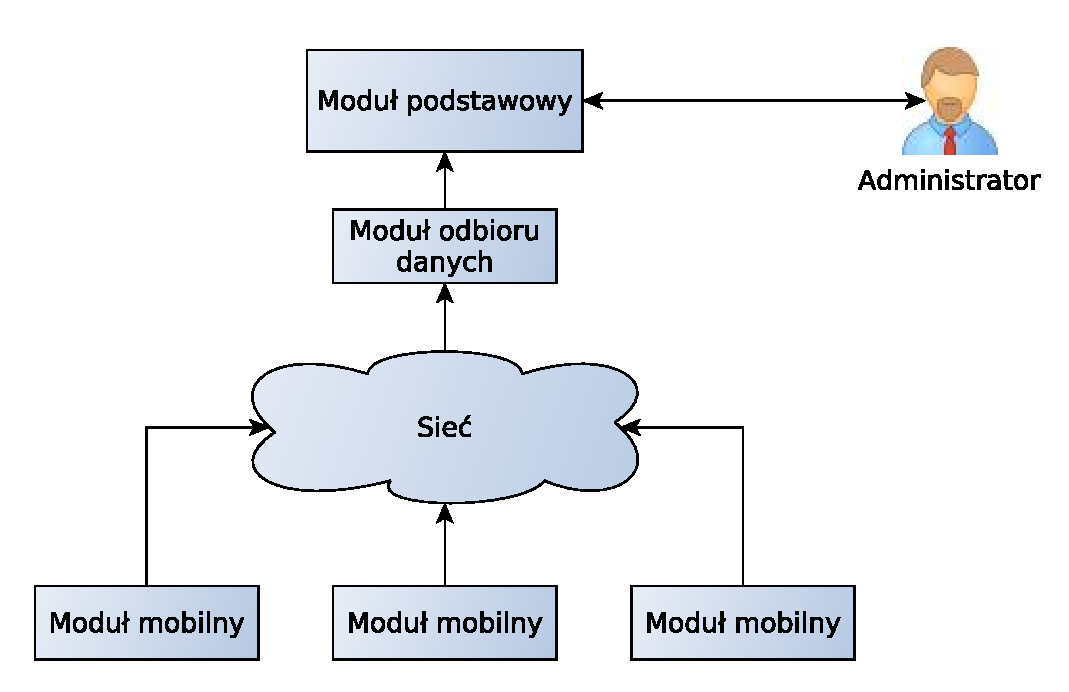
\includegraphics[width=0.8\textwidth]{img/archCalosci}
\end{figure}

\begin{description}
\item[Moduł podstawowy] Zawiera wszystkie instancje rdzenia
  monitorującego, zarówno te wykorzystywane do monitorowania
  infrastruktury statycznej, jak i~te których zadaniem jest
  przetwarzanie danych pochodzących od klientów mobilnych. Ponadto
  w~module tym zawiera się interfejs użytkownika wraz ze~wszystkimi
  dodatkami oraz magazyn danych.

\item[Moduł odbioru danych] Składa się on z~programu, który zapewnia
  odbiór danych od klienta mobilnego przy zachowaniu wszystkich
  wymagań zarówno w~kwestii bezpieczeństwa jak
  i~funkcjonalności. Ponadto moduł ten odpowiedzialny jest za
  przekazywanie odebranych danych do pozostałych elementów zgodnie
  ze~zdefiniowaną w~systemie polityka.

\item[Moduł mobilny] Zależna od platformy aplikacja mobilna, której
  podstawowym zadaniem jest gromadzenie danych o~zadanych
  parametrach. Zawiera się tu również implementacja protokołu
  komunikacyjnego dla danej platformy w~celu przekazania zebranych
  danych do pozostałych modułów systemu.
\end{description}

\section[Projekt modułu podstawowego][Projekt modułu podstawowego]{Projekt modułu podstawowego}

Moduł ten składa się z~kilku współpracujących ze sobą
elementów. Możliwa jest konfiguracja tego modułu w~kilku wariantach,
co umożliwia dostosowanie go do rozmiarów oraz topologi monitorowanej
infrastruktury. Każda z~stosowanych konfiguracji musi zapewniać
co najmniej poniższą funkcjonalność:

\begin{itemize}
\item monitorowanie infrastruktury statycznej,
\item przetwarzanie danych pochodzących od klienta mobilnego,
\item gromadzenie danych,
\item zapewnienie interfejsu dla administratora.
\end{itemize}

Minimalna konfiguracja modułu musi się składać co najmniej z~jednej
instancji rdzenia monitorującego oraz dowolnego z~interfejsów,
klasycznego lub icinga-web. W~celu umożliwienia przetwarzania danych
pochodzących od klientów mobilnych konieczne jest jedynie
zdefiniowanie tych urządzeń oraz ich usług, jako monitorowane
pasywnie. Należy jednak zwrócić uwagę na liczne ograniczenia tej
konfiguracji, które zostały omówione w~\ref{chap:Icinga}. Ponadto
konfiguracja ta nie spełnia wszystkich wymagań, gdyż nie umożliwia
analizy zgromadzonych danych historycznych. W~celu spełnienia
wszystkich wymagań należy zatem wzbogacić omawianą konfigurację
o~dodatek inGraph, który umożliwi administratorowi analizę
zgromadzonych danych.

Liczne wady przedstawionej konfiguracji powodują, że jej
funkcjonalność jest znacząco ograniczona. Wykorzystanie jej możliwe
jest jedynie w~bardzo małych sieciach, które nie będą już
rozwijane. Zalecana jest zatem konfiguracja o~nieco rozszerzonej
strukturze. W~skład tej konfiguracji wchodzą:

\begin{itemize}
\item rdzeń lub rdzenie monitorujące z~komponentem IDOUtils
\item baza danych systemu Icinga
\item dodatek inGraph
\item baza danych dodatku inGraph
\item interfejs icinga-web
\end{itemize}

\begin{figure}[ht]
\centering
  \caption{Schemat zalecanej konfiguracji systemu.}
  \label{fig:modulPodstawowy}
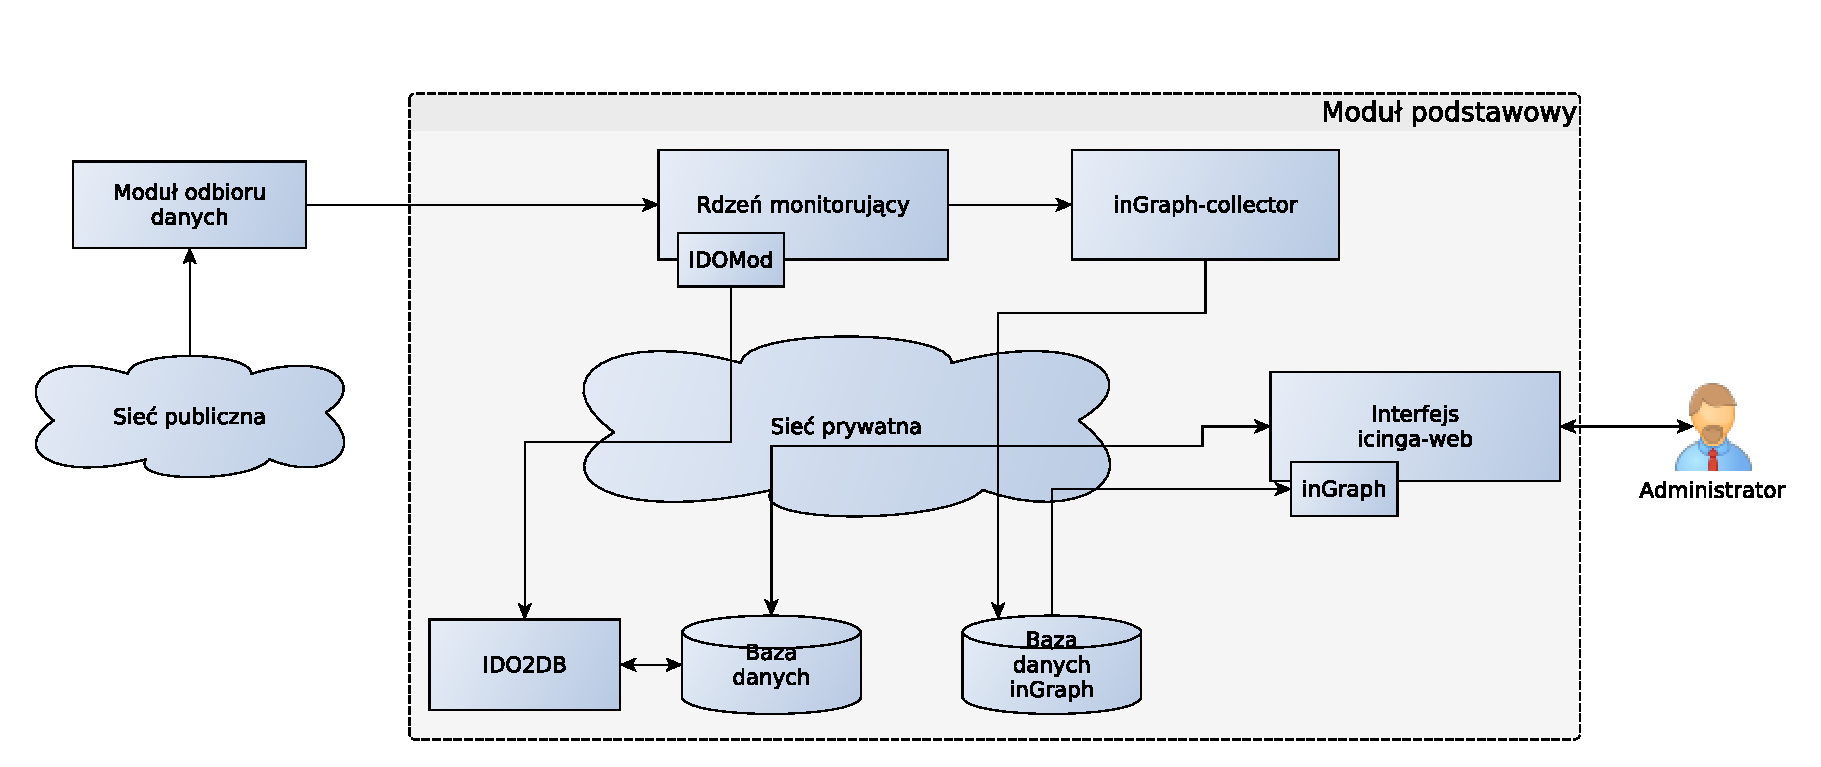
\includegraphics[width=1\textwidth]{img/modulPodstawowy}
\end{figure}

Minimum wymaganym do funkcjonowania tej konfiguracji jest jedna
instancja rdzenia monitorującego. Będzie ona monitorowała zarówno
infrastrukturę statyczną jak i~przetwarzała dane od klienta
mobilnego. Wszystkie dane przetworzone przez tą instancję trafiają do
bazy danych z~której korzysta interfejs użytkownika icinga-web. Taka
konfiguracja umożliwia bardzo dobrą skalowalność całego systemu oraz
łatwego dostosowania go do struktury monitorowanej sieci. Rozbudowa
infrastruktury monitorującej może zostać wykonana w~łatwy sposób
poprzez dodanie kolejnej instancji jądra wykorzystującej tą samą bazę
danych. Ponadto możliwe jest również łączenie tej konfiguracji
z~niemalże dowolną inną konfiguracją bez zaburzania pracy
systemu. Skalowalność tej konfiguracji dotyczy również klienta
mobilnego. Jeśli klientów mobilnych jest zbyt dużo, aby mogły zostać
obsłużone przez jedną instancję, możliwe jest dodanie kolejnej
instancji, która będzie odpowiedzialna za przetwarzanie danych od
wyznaczonej części klientów mobilnych. W~celu umożliwienia analizy
danych historycznych zalecane jest użycie dodatku inGraph. Został on
opisany szczegółowo w~\ref{sec:inGraph}. Jego wykorzystanie umożliwia
prezentację administratorowi zarówno uśrednionych wartości z~długiego
okresu czasu jak i~szczegółowych danych z~zadanego przedziału. W~celu
wykorzystania tego dodatku w~omawianej konfiguracji konieczne jest
umieszczenie elementu zbierającego dane przy każdej instancji rdzenia
monitorującego. Wszystkie zebrane dane zapisywane są w~jednej bazie
danych z~której korzysta interfejs użytkownika.



\section[Protokół komunikacyjny][Protokół komunikacyjny]{Protokół komunikacyjny}
\label{sec:ProtKom}

Wymagania przedstawione w~\ref{chap:Wymagania} definiują bardzo wiele
cech systemu, które muszą być zapewnione poprzez użycie odpowiedniego
protokołu komunikacyjnego. Analiza wymagań pozwoliła na wyodrębnienie
następujących cech protokołu komunikacyjnego:

\begin{description}
\item[spójność danych] protokół musi gwarantować, że dane zostały
  dostarczone i~przetworzone;
\item[integralność] protokół musi zapewniać, że dane zostaną
  dostarczone w~niezmodyfikowanej postaci i~jedynie od
  uwierzytelnionego nadawcy;
\item[poufność] protokół musi zapewniać przekazanie danych w sposób,
  który uniemożliwi stroną trzecim ich odczytanie;
\item[niezależność algorytmu szyfrowania] protokół musi być niezależny
  od algorytmu, którym szyfrowane są dane;
\item[uwierzytelnienie klienta] protokół musi zapewniać element
  pozwalający na potwierdzenie tożsamości klienta;
\item[niezależność uwierzytelnienia klienta] protokół musi być
  niezależny od wykorzystywanej metody uwierzytelnienia klienta;
\item[uwierzytelnienie serwera] protokół musi zapewniać potwierdzenie
  tożsamość serwera;
\item[odporność na utratę urządzenia klienckiego] protokół nie może
  wymagać przechowywania na urządzeniu danych pozwalających na
  kompromitację całego systemu;
\item[oszczędność pasma] protokół powinien minimalizować ilość
  przesyłanych danych.
\end{description}

Rozbudowane wymagania bezpieczeństwa protokołu wynikają
z~charakterystyki przesyłanych danych. Dane, które pochodzą
z~urządzenia mogą zawierać zarówno poufne dane właściciela jak
i~tajemnice handlowe firmy. Ujawnienie tych danych może pociągać za
sobą poważne konsekwencje finansowe lub prawne, dlatego konieczne jest
zapewnienie bezpiecznego protokołu. Należy również pamiętać, że jedna
ze stron komunikujących się przy użyciu protokołu znajduje się na
urządzeniu mobilnym przez co należy ograniczyć narzut wprowadzany
przez użycie tego protokołu.

Spośród bezpiecznych protokołów komunikacyjnych rozpowszechnionych na
rynku najbliższym spełnienia wszystkich wymagań jest protokół Secure
Socket Layer - SSL\footnote{Szczegółowy opis protokołu można znaleźć
  w~\cite[148-155]{book:kryptografia}.}. Jest to protokół warstwy
prezentacji, który pozwala na bezpieczny transport strumienia
danych. Protokół wykorzystuje zarówno kryptografię symetryczną jak
i~asymetryczną. Kryptografia asymetryczna wykorzystywana jest do
uwierzytelnienia serwera i~opcjonalnie klienta przy pomocy
certyfikatów nadawanych przez centra certyfikacji. Model
bezpieczeństwa zastosowany w~tym protokole pozwala przy pomocy kluczy
centrów autoryzacji dokonywać weryfikacji certyfikatów przesyłanych
przez wiele witryn. Niestety głębsza analiza protokołu wykazała, iż
nie spełnia on wszystkich wymagań. Przede wszystkim zestawienie
połączenia wymaga przesłania znaczącej ilości danych. Ponadto
konieczne jest zdobycie certyfikatu, który pozwalałby na weryfikację
serwera. Model bezpieczeństwa zastosowany w~SSL jest dla
rozpatrywanego przypadku nadmiarowy, ponieważ klient mobilny
przekazuje dane zawsze do tego samego serwera. Protokół SSL
przeznaczony jest głównie dla sklepów internetowych oraz banków, gdyż
jest on nastawiony na uwierzytelnienie serwera i~zapewnia bezpieczny
kontakt w wieloma domenami przy użyciu niewielkiej liczby centrów
certyfikujących.

Nadmiarowość modelu bezpieczeństwa protokołu SSL powoduje nadmierne
zużycie pasma. Ponadto zamknięty zbiór algorytmów możliwych
szyfrowania możliwych do wykorzystania powoduje, że nie może on być
zastosowany w~omawianym przypadku. Wobec braku gotowego protokołu
konieczne jest zaprojektowanie nowego, który spełni wszystkie stawiane
wymagania.

Protokół został oparty na protokole TCP, który zapewnia abstrakcję
przesłania strumienia bajtów z~gwarancją ich dostarczenia. Mnogość
wymagań dotyczących projektowanego protokołu utrudnia wykorzystanie
architektury jednowarstwowej. Konieczne jest zatem wydzielenie warstw
z~których każda będzie zapewniała dobrze zdefiniowane usługi dla
warstw wyższych.
 

\subsection[Warstwa formowania wiadomości][Warstwa formowania wiadomości]{Warstwa formowania wiadomości}

Najniższa warstwa protokołu komunikacyjnego zbudowana jest
bezpośrednio na protokole TCP. Komunikujące się strony w swej
architekturze wykorzystują paradygmat programowania
zdarzeniowego. Abstrakcja strumienia bajtów zapewniana przez protokół
TCP nie jest odpowiednia dla tego modelu. Konieczne jest zatem
dostarczenie warstwy, która umożliwi przesłanie w całości komunikatu
o~zadanej długości. Umożliwia to wygodne przesyłanie wiadomości
odpowiadających poszczególnym zdarzeniom w~komunikujących się
programach.

Usługa zapewniana przez tą warstwę jest bardzo prosta, dzięki czemu
rozpoczęcie komunikacji nie wymaga żadnej inicjalizacji. Protokół jest
w~pełni symetryczny. Oznacza to, że obie komunikujące się strony
posiadają taki sam dozwolony zbiór stanów protokołu. Warstwa świadczy
usługę przekazywania wiadomości o~zdefiniowanym rozmiarze. W~celu
wykonania tej usługi, do danych, które są dostarczone stronie
nadawczej dołączana jest ich długość. Długość w~protokole jest
reprezentowana jako 32 bitowa liczba ze znakiem o~sieciowej kolejności
bajtów. Tak sformatowana wiadomość przesyłana jest przy użyciu
protokołu TCP do odbiorcy. Odbiorca po odebraniu pierwszych czterech
bajtów wiadomości sprawdza rozmiar danych, po czym rozpoczyna
odbieranie ilości danych określonej przez nagłówek. Wiadomość jest
przekazywana użytkownikowi dopiero w~momencie odebrania całego
komunikatu. Jeśli w~trakcie odbierania fragmentów wiadomości nastąpi
przerwanie połączenia, odebrane fragmentu wiadomości są porzucane,
a~użytkownikowi sygnalizowany jest błąd.

\begin{table}[H]
\centering
\caption{Struktura komunikatu warstwy formowania wiadomości}

\begin{tabular}{|p{3cm}|p{6cm}|}
\hline
Długość danych & Dane\\
\hline
\end{tabular}
\end{table}

\subsection[Warstwa kryptograficzna][Warstwa kryptograficzna]{Warstwa kryptograficzna}

Warstwa ta jest odpowiedzialna za zapewnienie poufności oraz
integralności przesyłanych danych. Ponadto zadaniem tej warstwy jest
również wykonanie uwierzytelnienia serwera. Podczas projektowania tej
warstwy konieczne było uwzględnienie również wymagania, które zalecało
niezależność algorytmu szyfrowania przesyłanych danych od protokołu
komunikacyjnego. W~celu zapewnienia możliwości późniejszej modyfikacji
protokołu, warstwa ta zawiera również proces negocjacji wersji
protokołu.

Model bezpieczeństwa implementowany przez tą warstwę jest zbliżony do
protokołu SSL, jednak zostały wprowadzone zmiany, które zmniejszają
zużycie pasma oraz eliminują potrzebę wykorzystania
certyfikatów. Zanim możliwa będzie bezpieczna komunikacja z~użyciem
tej warstwy konieczne jest umieszczenie na urządzeniu mobilnym klucza
publicznego RSA oraz klucza prywatnego na serwerze. Istotne jest, aby
klucze mogły być umieszczane jedynie przez autoryzowaną osobę,
np. administratora tych urządzeń. Bezpośrednie umieszczenie klucza
publicznego serwera na urządzeniu eliminuje potrzebę wykorzystania
certyfikatów oraz ich przesyłania. Należy jednak zwrócić uwagę, iż w
przyjętym modelu nie jest możliwa zmiana klucza publicznego serwera
bez ponownego umieszczenia go na urządzeniu. Nie stanowi to jednak
problemu, gdyż zmiana klucza publicznego w~projektowanym systemie jest
sytuacją niezwykle rzadką. Ponieważ szyfrowanie asymetryczne wymaga
znacznie większego narzutu obliczeniowego jest ono używane tylko
w~trakcie nawiązywania połączenia. Właściwy transport danych
szyfrowany jest przy pomocy uzgodnionego klucza
symetrycznego. W~poniższym omówieniu protokołu, a~także na diagramach,
w~celu uproszczenia pominięto fakt istnienia limitu czasu oczekiwania
oraz możliwość rozłaczenia w~dowolnym momencie. Obie te sytuacje
powodują zakończenie działania i~zgłoszenie błędu warstwie
wyższej. Uproszczona wersja maszyny stanowej procesu incjalizacji
komunikacji w~tej warswie po stronie serwera znajduje się na
\ref{fig:kryptoSerwer}, a po stronie klienta \ref{fig:kryptoKlient}.

Komunikacja z~użyciem tej warstwy możliwa jest dopiero po wykonaniu
inicjalizacji. Proces inicjalizacji rozpoczyna się od negocjacji
używanej wersji protokołu. Niezwłocznie po nadejściu połączenia od
klienta serwer wysyła komunikat będący zapytaniem o~żądaną przez
klienta wersję protokołu. Klient odpowiada na ten komunikat
przesyłając żądaną wersję protokołu. Jeśli serwer może obsłużyć dana
wersję protokołu przesyła on pozytywne potwierdzenie do klienta, co
powoduje rozpoczęcie kolejnego etapu inicjalizacji. W~przeciwnym
przypadku serwer przesyła informację o~odrzuceniu żądania. Po
odebraniu negatywnego potwierdzenia klient może podjąć kolejne próby
używając innych wersji protokołu. Dalsza komunikacja uzależniona jest
od wybranej wersji protokołu komunikacyjnego.

\begin{table}[H]
\centering
\caption{Struktura komunikatu żądanie wersji}

\begin{tabular}{|p{5cm}|p{6cm}|}
\hline
\raggedright{Kod REQUEST\_PROTOCOL} & Nazwa wersji\\
\hline
\end{tabular}
\end{table}

\begin{figure}[h]
  \caption{Maszyna stanów warstwy kryptograficznej po stronie serwera.}
  \label{fig:kryptoSerwer}
  \centering
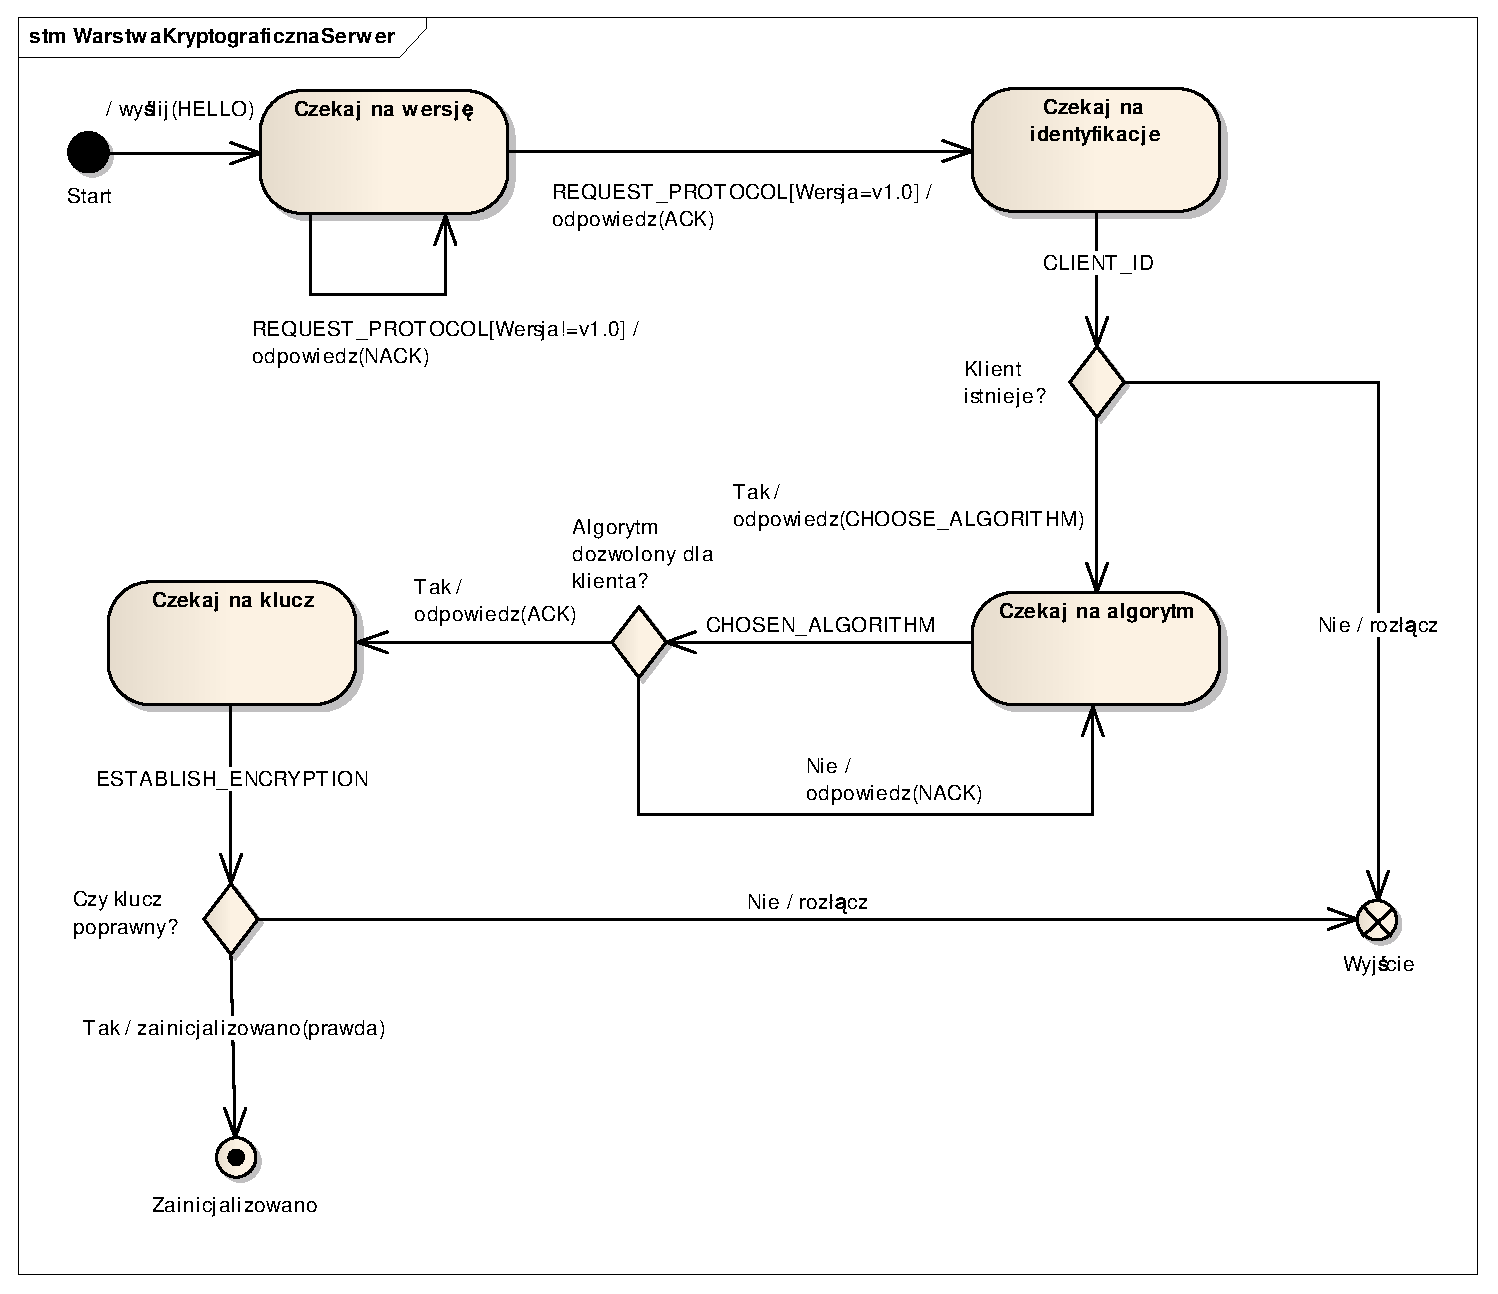
\includegraphics[width=1\textwidth]{img/kryptoSerwer}
\end{figure}

W~zaproponowanej w~tej pracy wersji protokołu kolejnym etapem
inicjalizacji połączenia jest uwierzytelnienie serwera połączone
z~przedstawieniem klienta. Etap ten rozpoczyna się od przesłania przez
klienta jego identyfikatora oraz losowych ośmiu bajtów
danych. Komunikat zaszyfrowany jest kluczem publicznym serwera, zatem
może go odczytać jedynie posiadacz odpowiedniego klucza
prywatnego. Serwer po odebraniu wiadomości odszyfrowuje ją używając
swojego klucza prywatnego. Jeśli wiadomość jest nieczytelna lub klient
o~podanym identyfikatorze nie istnieje serwer niezwłocznie kończy
połączenie. Jeśli wiadomość jest poprawna, a~klient o~podanym
identyfikatorze istnieje serwer wykonuje podpis cyfrowy identyfikatora
oraz losowych bajtów odebranych od klienta. Do klienta odsyłany jest
komunikat zawierający wykonany przez serwer podpis. Klient po
odebraniu podpisu wykonuje weryfikację podpisu na podstawie
wiadomości, która została przesłana do serwera. Jeśli podpis jest
zgodny oznacza to, że urządzenie z którym nastąpiło połączenie jest
posiadaczem odpowiedniego klucza prywatnego, czyli upoważnione przez
administratora do odbierania danych pochodzących od tego klienta.

\begin{figure}[h]
  \caption{Maszyna stanów warstwy kryptograficznej po stronie klienta.}
  \label{fig:kryptoKlient}
  \centering
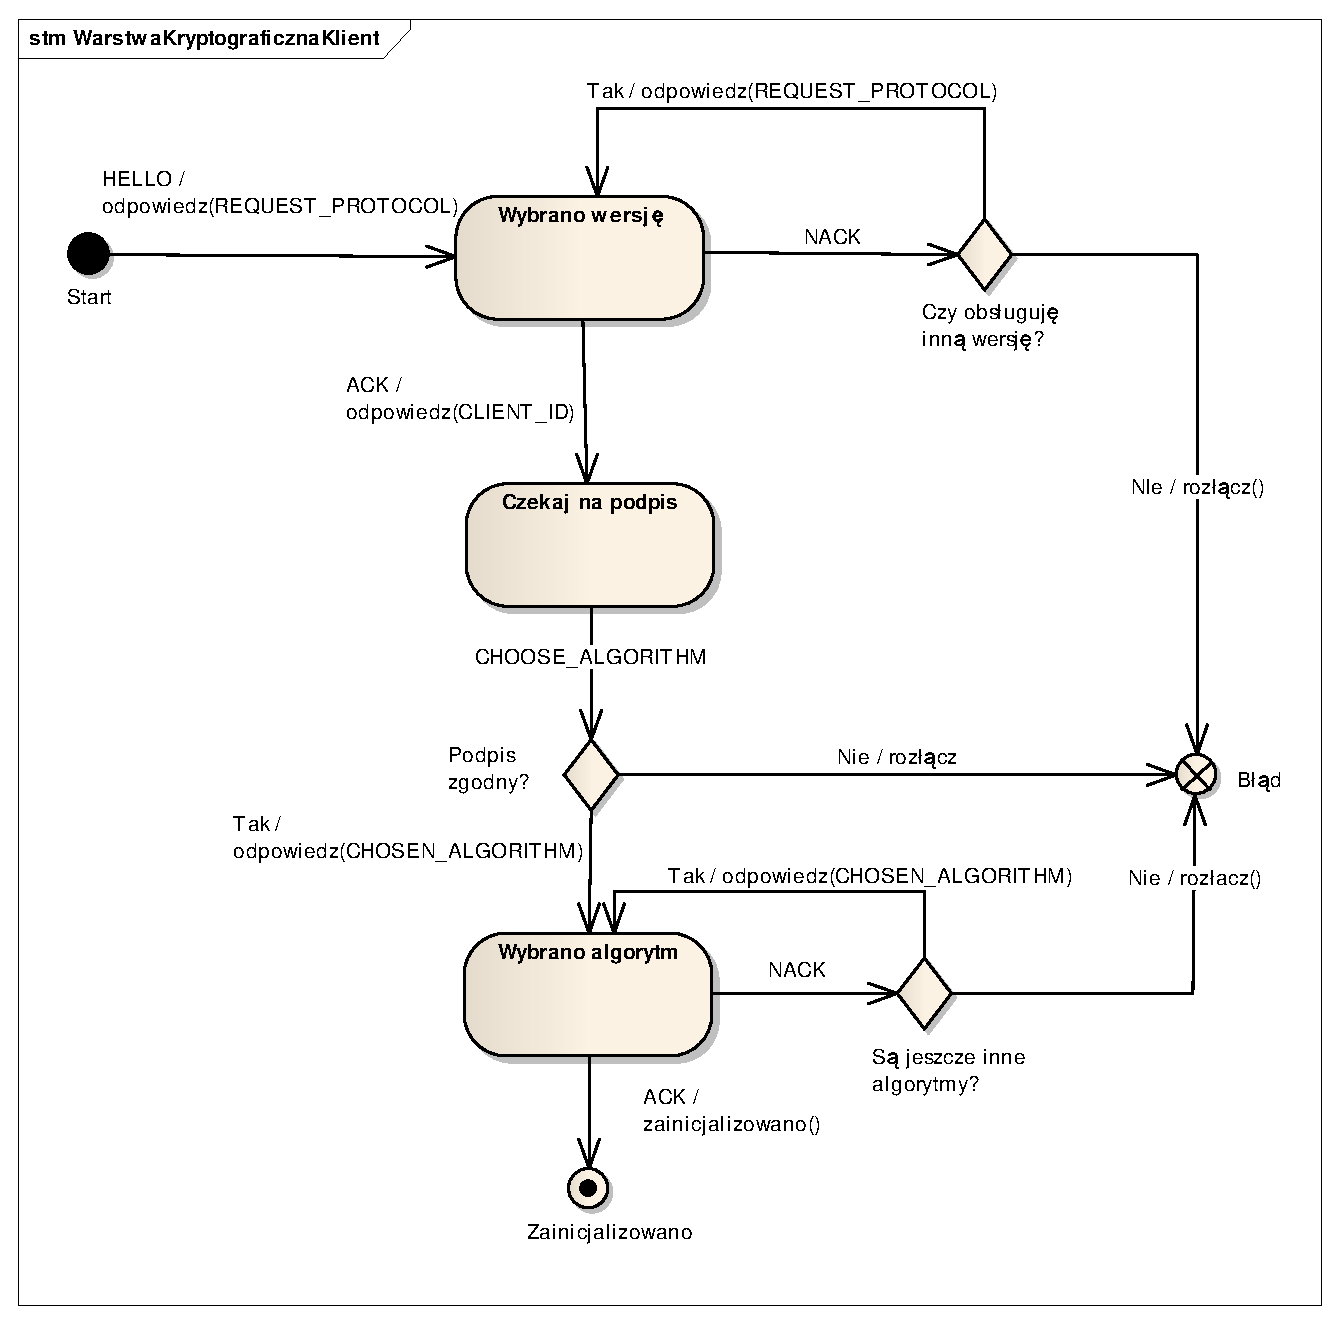
\includegraphics[width=1\textwidth]{img/kryptoKlient}
\end{figure}

\begin{table}[H]
\centering
\caption{Struktura komunikatu identyfikatora klienta }

\begin{tabular}{|p{3cm}|p{3cm}|p{6cm}|}
\hline
Kod CLIENT\_ID & Ciąg losowy & Identyfikator\\
\hline
\end{tabular}
\end{table}

\begin{table}[H]
\centering
\caption{Struktura komunikatu potwierdzającego identyfikator }

\begin{tabular}{|p{6cm}|p{6cm}|}
\hline
Kod CHOOSE\_ALGORITHM & Podpis danych z CLIENT\_ID\\
\hline
\end{tabular}
\end{table}

Ostatnim etapem inicjalizacji komunikacji w~tej warstwie jest
negocjacja algorytmu szyfrowania oraz generacja odpowiedniego klucza
symetrycznego. Klient przesyła do serwera zaszyfrowany kluczem
publicznym komunikat zawierający żądanie algorytmu
symetrycznego. Serwer po odebraniu komunikatu odszyfrowuje go przy
użyciu klucza prywatnego. W zależności od dostępności żądanego
algorytmu, do klienta odsyłany jest komunikat akceptujący lub
odrzucający wybrany algorytm. Klient po odebraniu negatywnego
potwierdzenia może ponownie zażądać innego algorytmu
symetrycznego. Klient po odebraniu komunikatu akceptującego wybrany
algorytm dokonuje generacji klucza symetrycznego, a~następnie oblicza
jego skrót. Tak przygotowany komunikat szyfrowany jest kluczem
publicznym i~przesyłany do serwera. Serwer po odebraniu klucza
sprawdza jego poprawność oraz zgodność z~dołączonym skrótem, co
stanowi ostatni etap inicjalizacji.

\begin{table}[H]
\centering
\caption{Struktura komunikatu żądania algorytmu }

\begin{tabular}{|p{5cm}|p{6cm}|}
\hline
\raggedright{Kod CHOSEN\_ALGORITHM} & Nazwa algorytmu\\
\hline
\end{tabular}
\end{table}

\begin{table}[H]
\centering
\caption{Struktura komunikatu zawierającego klucz symetryczny}

\begin{tabular}{|p{3cm}|p{5cm}|p{3cm}|p{2cm}|}
\hline
Długość skrótu & \raggedright{Kod ESTABLISH\_ENCRYPTION} & \raggedright{Klucz symetryczny} & Skrót \\
\hline
\end{tabular}
\end{table}

Wykonanie inicjalizacji pozwoliło na uzgodnienie w~sposób bezpieczny
klucza symetrycznego. W~dalszej komunikacji wszystkie komunikaty
szyfrowane są z~użyciem wybranego algorytmu symetrycznego. Ponieważ
algorytmy szyfrowania nie zapewniają integralności przesyłanych danych
konieczne jest użycie funkcji skrótu. W~omawianym protokole została
użyta funkcja SHA2. Przygotowanie zatem każdego komunikatu z~danymi
rozpoczyna się od obliczenia skrótu danych. Ponieważ algorytm skrótu
nie był negocjowany konieczne jest dostarczenie długości używanego
skrótu. Długość skrótu wyrażona w bajtach dołączana jest na początku
wiadomości, natomiast sam skrót na końcu. Komunikat przed wysłaniem
szyfrowany jest uzgodnionym kluczem symetrycznym.

\begin{table}[H]
\centering
\caption{Struktura komunikatu danych warstwy kryptograficznej }

\begin{tabular}{|p{3cm}|p{6cm}|p{3cm}|}
\hline
Długość skrótu & Dane & Skrót danych\\
\hline
\end{tabular}
\end{table}

\subsection[Warstwa transportu pomiarów][Warstwa transportu pomiarów]{Warstwa transportu pomiarów}

Warstwa ta zapewnia zapewnia transport wpisów dziennika w~pakietach
o~dowolnym rozmiarze. Wykorzystanie warstw niższych gwarantuje zarówno
poufność jak i~integralność przesyłanych komunikatów. Żadna z~niższych
warstw nie zapewnia jednak uwierzytelnienie klienta, dlatego jest to
również jedno z~zadań tej warstwy.

Inicjalizacja komunikacji w~tej warstwie rozpoczyna się od negocjacji
algorytmu uwierzytelnienia klienta. Serwer przesyła do klienta
komunikat informujący o~konieczności wyboru algorytmu
uwierzytelnienia. Klient przesyła komunikat zawierający nazwę
algorytmu, który ma być użyty do potwierdzenia tożsamości. Serwer po
otrzymaniu komunikatu sprawdza czy żądany algorytm jest dostępny dla
tego klienta. Jeśli nie jest, przesyłany jest komunikat informujący
o~odrzuceniu żądania, a~klient może ponowić żądanie używając innego
algorytmu. Jeśli algorytm wybrany przez klienta jest dostępny
rozpoczyna się proces uwierzytelnienia.

\begin{table}[H]
\centering
\caption{Struktura komunikatu żądania algorytmu uwierzytelnienia }
\begin{tabular}{|p{5cm}|p{6cm}|}
\hline
\raggedright{Kod CHOSEN\_AUTH\_MODULE} & Nazwa algorytmu uwierzytelnienia\\
\hline
\end{tabular}
\end{table}

Uwierzytelnienie klienta wykonywane jest poprzez zewnętrzne moduły,
gdyż protokół komunikacyjny musi być niezależny od protokołu
komunikacyjnego. Algorytm uwierzytelnienia uprawniony jest do
przesyłania dowolnych danych w~obie strony. Jeśli algorytm
uwierzytelnienia odrzuci klienta oznacza to natychmiastowe zamknięcie
połączenia. Pomyślne zakończenie procesu uwierzytelnienia oznacza,
konieczność wykonania sprawdzenia, czy klient posiada zdefiniowane
miejsca do których może przekazywać swoje dane. W przypadku braku
takiego miejsca, aby dane nie zostały utracone do klienta wysyłany
jest komunikat negatywnego potwierdzenia, a~połączenie jest
zamykane. Jeśli co najmniej jedno miejsce docelowe zostało
zdefiniowane do klienta wysyłany jest komunikat informujący
o~oczekiwaniu na przesłanie danych, co kończy proces
inicjalizacji. Przebieg omówionego procesu inicjalizacji oraz
pozostałych elementów protokołu po stronie serwera przedstawia
\ref{fig:transportSerwer}, natomiast po stronie klient
\ref{fig:transportKlient}.


\begin{figure}[ht]
  \caption{Maszyna stanów warstwy transportu pomiarów po stronie serwera.}
  \label{fig:transportSerwer}
  \centering
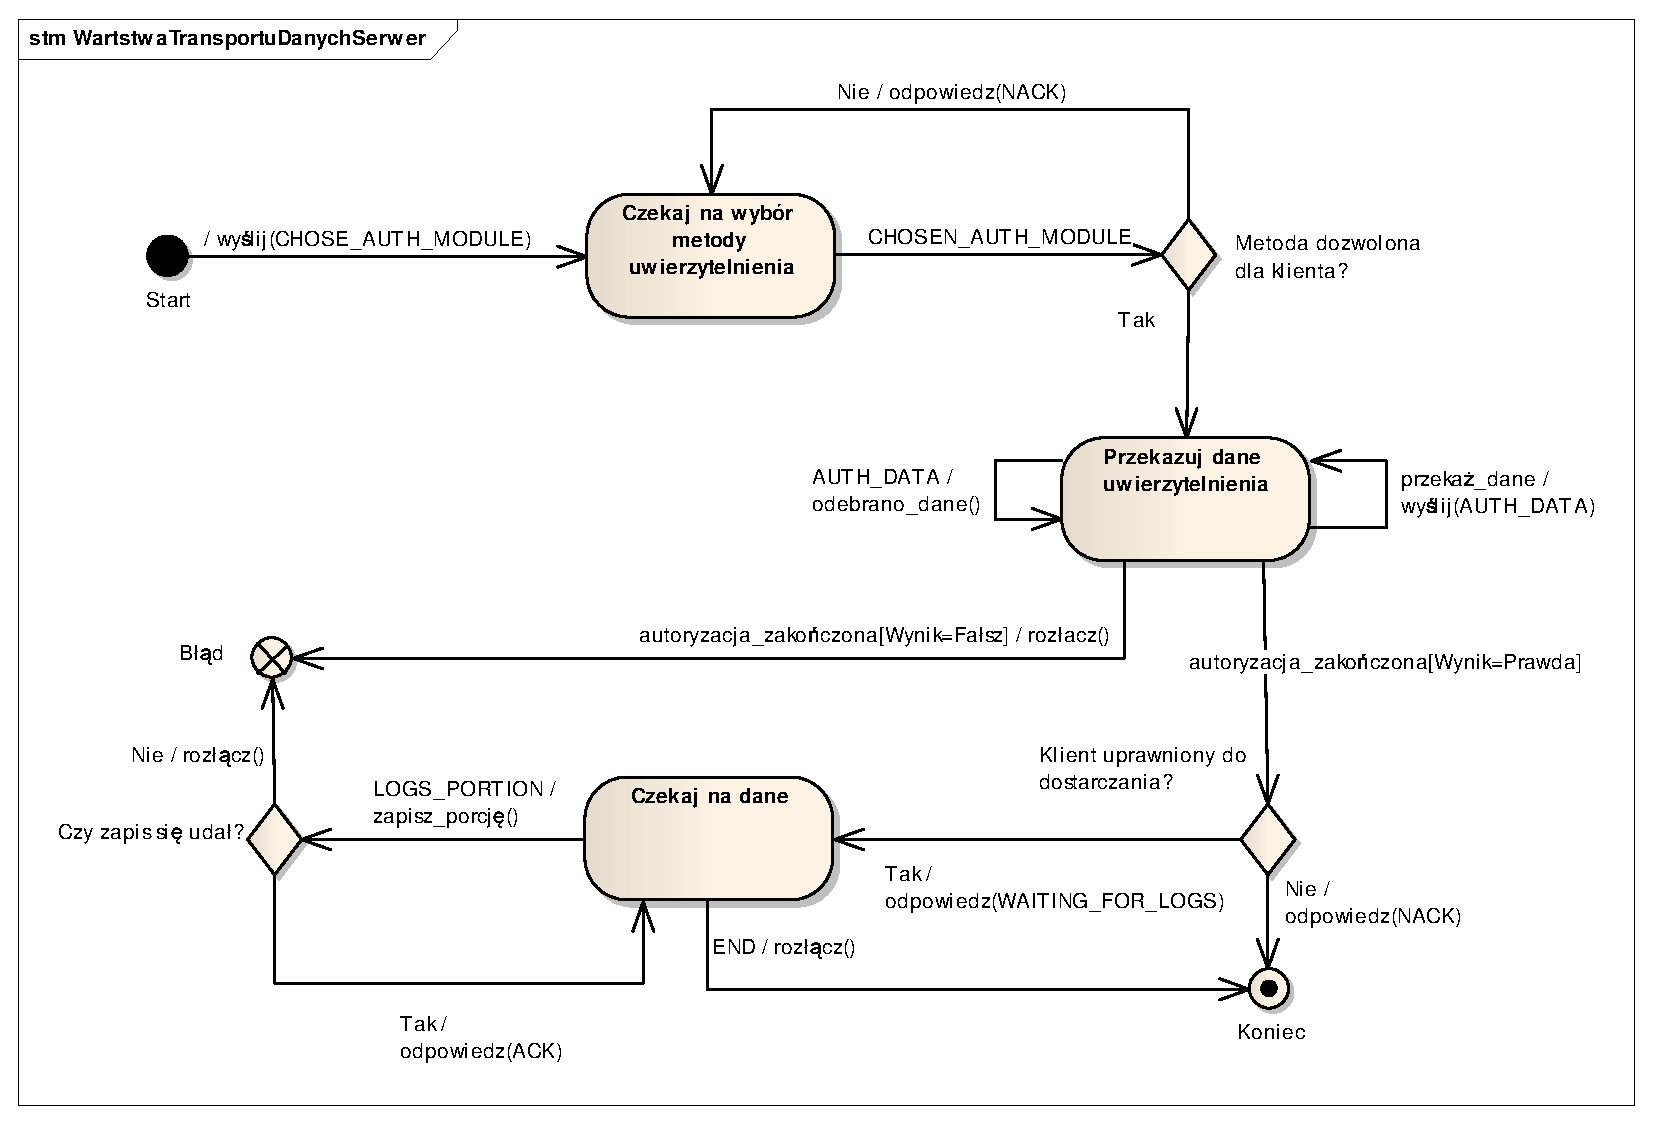
\includegraphics[width=1\textwidth]{img/transpSerwer}
\end{figure}

\begin{figure}[ht]
  \caption{Maszyna stanów warstwy transportu pomiarów po stronie klienta.}
  \label{fig:transportKlient}
  \centering
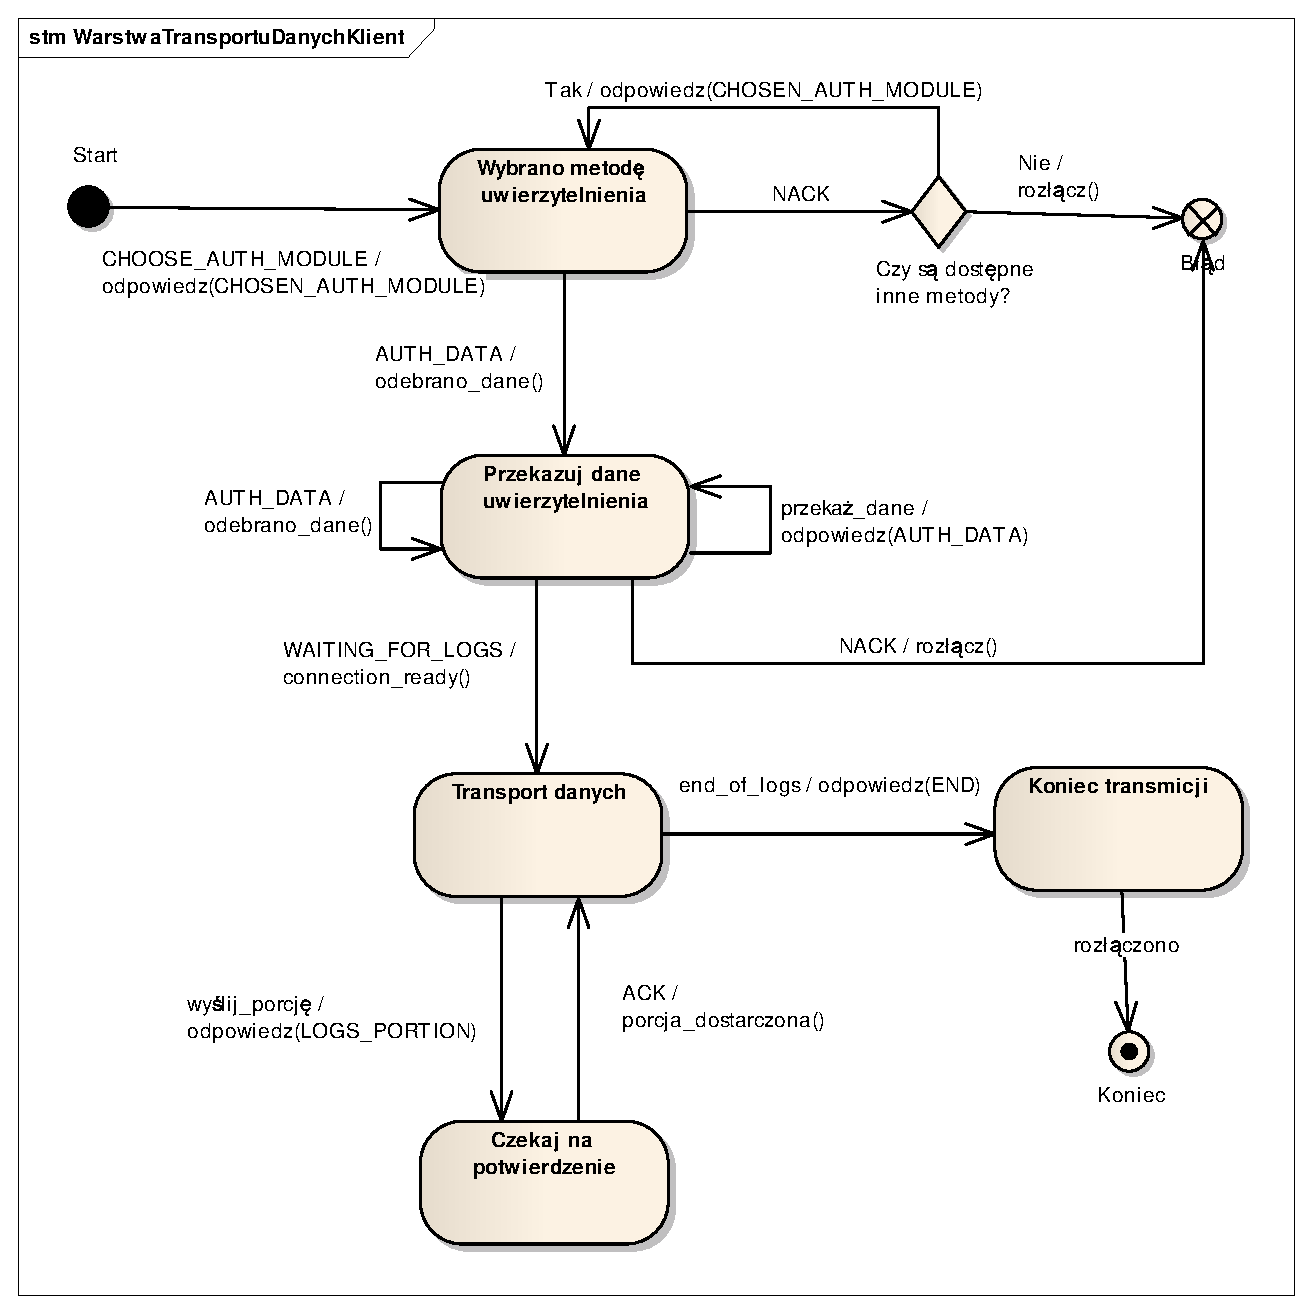
\includegraphics[width=1\textwidth]{img/transpKlient}
\end{figure}

\begin{table}[H]
\centering
\caption{Struktura komunikatu z danymi uwierzytelnienia }
\begin{tabular}{|p{3cm}|p{6cm}|}
\hline
Kod AUTH\_DATA & Dane \\
\hline
\end{tabular}
\end{table}

Dane przesyłane przez klienta znajdują się w pakietach. Po odebraniu
każdego pakietu i~jego pomyślnym przetworzeniu przez aplikację
obliczany jest skrót danych w~nim zawartych. Obliczony skrót jest
następnie przesyłany w~pakiecie potwierdzającym przetworzenie danych.

\begin{table}[H]
\centering
\caption{Struktura komunikatu zawierającego dane }
\begin{tabular}{|p{3cm}|p{6cm}|}
\hline
\raggedright{Kod LOGS\_PORTION} & Dane pomiarów  \\
\hline
\end{tabular}
\end{table}

Pakiet z~danymi może zawierać dowolną liczbę wpisów dziennika. Każdy
wpis powinien posiadać odpowiedni format. W~szczególności każdy wpis
powinien zawierać bajt danych, który pozwala na określenie czy dotyczy
on urządzenia czy usługi. Niezbędne jest również przesłanie stempla
czasu, który determinuje kiedy dany wpis został utworzony. Stempel ten
powinien być zgodny z stemplem czasu systemu Unix oraz być przesłany w
sieciowej kolejności bajtów. Do prawidłowego przekazania wpisu do
systemu monitorującego konieczne jest również dostarczenie nazwy
urządzenia oraz usługi. W~celu umożliwienia oddzielenia tych danych
konieczne jest zakończenie każdego z~tych pól znakiem zerowym. Każdy
wpis powinien również zawierać bajt informujący o~stanie w~jakim jest
dana usługa. Kod ten powinien być zapisany przy użyciu jednego bajtu
w~sposób zgodny z~kodami akceptowanymi przez system monitorujący.

\begin{table}[H]
\centering
\caption{Struktura pojedynczego wpisu dziennika urządzenia }
\begin{tabular}{|p{2cm}|p{3cm}|p{4cm}|p{2cm}|p{2cm}|}
\hline
Kod HOST & Stempel czasu & Nazwa urządzenia & Kod stanu & Wpis  \\
\hline
\end{tabular}
\end{table}

\begin{table}[H]
\centering
\caption{Struktura pojedynczego wpisu dziennika usługi }
\begin{tabular}{|p{2cm}|p{2cm}|p{3cm}|p{2cm}|p{1cm}|p{2cm}|}
  \hline
  \raggedright{Kod SERVICE} & \raggedright{Stempel czasu} & \raggedright{Nazwa urządzenia} & \raggedright{Nazwa usługi} & \raggedright{Kod stanu} & Wpis  \\
  \hline
\end{tabular}
\end{table}

Jeśli odebrane dane posiadają nieprawidłową strukturę, lub klient
dokonał próby przesłania danych, do których przesyłania nie ma
uprawnień połączenie jest natychmiast zamykane. Klient, po przesłaniu
wszystkich danych lub w~chwili zdefiniowanej przez administratora może
zdecydować o~zamknięciu połączenia wysyłając odpowiedni
komunikat. Serwer po odebraniu tego komunikatu zamknie połączenie.


\section[Projekt modułu mobilnego][Projekt modułu mobilnego]{Projekt modułu mobilnego}

Moduł ten jest odpowiedzialny za monitorowanie zadanych parametrów
urządzenia mobilnego. Klienty mobilne są wzajemnie nie zależne i~mogą
operować bez możliwości komunikacji pomiędzy sobą. Konieczne jest
zatem, aby każdy klient mobilny posiadał swoją instancję tego
modułu. W~module tym możemy wyróżnić trzy podstawowe, rozdzielne
funkcjonalnie elementy:

\begin{itemize}
\item element pomiarowy,
\item element komunikacyjny,
\item zestaw wtyczek.
\end{itemize}

Element pomiarowy jest odpowiedzialny za planowanie i~wykonywanie
pomiarów zgodnie z~polityką zdefiniowaną przed administratora. Ponadto
konieczne jest zapewnienie składowania uzyskanych informacji do czasu
udanej synchronizacji z~serwerem. Element komunikacyjny jest to
implementacja opisanego wcześniej protokołu komunikacyjnego dla danej
platformy. Zadaniem tej części jest dostarczenie wyników pomiarów do
miejsc zdefiniowanych przez administratora. Wtyczki są to elementy
bezpośrednio odpowiedzialne za wykonywanie pomiarów zadanych wartości
czy testowanie zdefiniowanych usług. Metoda realizacji wtyczek
uzależniona jest od platformy sprzętowej na jaką przeznaczona jest
dana implementacja modułu. Konieczne jest jednak zapewnienie
niezależności elementu pomiarowego od zestawu wykorzystywanych
wtyczek, aby umożliwić swobodną zmianę zbioru wykorzystywanych
wtyczek.

Implementacja tego modułu musi uwzględniać uwarunkowania sprzętowe jak
i~systemowe platformy na której się znajduje. Urządzenia mobilne są
zazwyczaj zasilane z~własnych akumulatorów dlatego konieczne jest
zastosowanie mechanizmów, które pozwolą na zredukowanie zużycia
energii związanego z~systematycznym wykonywaniem sprawdzeń. Należy
również wspomnieć, iż moduł mobilny odpowiedzialny jest za nadawanie
każdemu z~odczytów stempla czasu uniwersalnego\footnote{Czas
  uniwersalny - średni astronomiczny czas słoneczny na południku
  zerowym.} dokonywanego pomiaru. Na podstawie dokonanej
charakterystyki klienta mobilnego, można poczynić założenie, iż klient
posiada dostęp do punktów synchronizacji czasu. Jest wiele dostępnych
metod synchronizacji czasu na urządzeniu mobilnym, między innymi
pobranie czasu z~sieci GSM czy też z~serwerów czasu światowego, przez
co nie stanowi to dla klienta mobilnego poważnego wymagania.

Klient mobilny po zebraniu porcji wpisów dziennika o~rozmiarze zgodnym
z~polityką administratora, lub po upływie określonego czasu powinien
przesłać posiadane wpisy dziennika do modułu odbiorczego, a~po
uzyskaniu potwierdzenia usunąć je z~urządzenia w~celu oszczędności
pamięci. Możliwa jest również sytuacja, w~której klient mobilny
użytkowany jest przez pewien czas bez dostępu do sieci przez którą
możliwa jest komunikacja z serwerem. W takiej sytuacji moduł mobilny
powinien gromadzić odczyty, aż do czasu uzyskania możliwości
połączenia z~serwerem. Różnorodność platform dostępnych na rynku
sprawia, iż nie można wymagać od modułu odbiorczego dostarczenia
uniwersalnej implementacji protokołu komunikacyjnego. Wymaga się
zatem, aby klient mobilny używał protokołu komunikacyjnego zgodnego
z~protokołem modułu odbiorczego. Konieczne jest również, aby klient
mobilny posiadał możliwość definiowania metod uwierzytelnienia. Należy
również zapewnić możliwość weryfikacji tożsamości serwera, z~którym
nawiązuje się połączenie.

W~ramach systemu monitorowania możliwe jest funkcjonowanie wielu
instancji modułu mobilnego. Instancje te mogą być uruchomione na
bardzo wielu platformach. W~chwili pisania tej pracy nie znaleziono na
rynku żadnej aplikacji przeznaczonej, na platformę mobilną, która
spełniałaby stawiane wymagania. Szczegółowy projekt oraz
implementacja tego modułu dla platformy mobilnej wykracza poza zakres
niniejszej pracy. Podczas okresu testowania wykonanego systemu
wykorzystano moduł mobilny, przeznaczony dla platformy Android. Został
on zaprojektowany i~zaimplementowany przez Pana Marcina
Kubika. Szczegółowy opis tej implementacji klienta mobilnego można
znaleźć w~\cite{book:pracaKubika}.

\section[Projekt modułu odbiorczego][Projekt modułu odbiorczego]{Projekt modułu odbiorczego}
\label{sec:ProjModOdb}

Moduł ten pośredniczy w~przekazywaniu danych pomiędzy modułem mobilnym
a~modułem podstawowym. Uruchomiony jest on na serwerze, który posiada
dostęp do zarówno do sieci wewnętrznej instytucji, jak i~do sieci,
w~której funkcjonują klienty mobilne, w~szczególności do sieci
Internet. Możliwe jest również umieszczenie tego modułu na tym samym
urządzeniu, co rdzeń monitorujący odpowiedzialny z~przetwarzanie
danych pochodzących od klientów mobilnych.

Moduł ten składa się z jednego programu, którego zadaniem jest
przekazywanie danych od klientów mobilnych zgodnie ze zdefiniowaną
polityką. Znaczna część logiki programu oraz polityka dostarczania
danych jest konfigurowana przy pomocy pliku konfiguracyjnego, co
umożliwia jej zmianę bez konieczności ponownej kompilacji
programu. Plik ten zawiera również definicję klientów, którzy są
uprawnieni do przekazywania danych. Każdy klient może posiadać wiele
urządzeń, a każde z~urządzeń wiele usług. Zgodnie z~protokołem
komunikacyjnym przed przesłaniem danych występuje etap
uwierzytelnienia klienta. Przekazywanie danych możliwe jest jedynie po
zakończeniu pozytywnym potwierdzeniu tożsamości
klienta. Wysokopoziomowy model logiczny omawianego programu składa się
zatem z~następujących elementów:

\begin{itemize}
\item dostawca danych,
\item kanał komunikacyjny,
\item konsument danych.
\end{itemize}

Dostawca danych jest to fragment programu odpowiedzialny za odebranie
oraz kontrolę danych pochodzących od klienta. Zawiera on więc
implementację protokołu komunikacyjnego oraz wykorzystuje dostępne
w~programie algorytmy kryptografii oraz uwierzytelnienia zgodnie
z~konfiguracją. W celu umożliwienia współpracy różnych protokołów
komunikacyjnych możliwe jest używanie jednocześnie wielu dostawców
danych. Kanał komunikacyjny stanowi natomiast niezawodne
asynchroniczne medium komunikacyjne pomiędzy dostawcą, a
konsumentami. Dostawca danych zobowiązany jest do dostarczenia danych
jedynie do jednego miejsca, czyli kanału komunikacyjnego. Logika
zawarta w~kanale wyznacza natomiast na podstawie zdefiniowanej
polityki podzbiór konsumentów danych, którzy powinni powinien otrzymać
przekazane danych. Możliwe jest definiowanie polityki dostarczania
danych zarówno na podstawie informacji o~kliencie od którego pochodzą
dane, jak i~na podstawie informacji o~dostawcy który odebrał
dane. W~celu przyśpieszenia komunikacji z~klientem mobilnym
potwierdzenie przetworzenia danych zawarte w~protokole komunikacyjnym
wysyłane jest niezwłocznie po przekazaniu danych do kanału
komunikacyjnego. Konieczne jest zatem zapewnienie niezawodności kanału
komunikacyjnego, aby możliwe było gwarantowanie, że dane, które do
niego zostały przekazane będą dostarczone do wskazanych
odbiorców. Odbiorca danych jest to element programu odpowiedzialny za
odpowiednie formowanie danych oraz przekazanie ich do modułu
podstawowego. Dzięki możliwości dostarczania danych do wielu
odbiorców, możliwe jest nie tylko przekazywanie danych do systemu
monitorującego lecz również wykonywanie np. kopi zapasowej otrzymanych
danych. Przykłądowy schemat logiczny dla dwóch dostawców danych oraz
trzech konsumentów został przedstawiony na \ref{fig:odbiorczy}

\begin{figure}[ht]
  \caption{Diagram architektury modułu odbiorczego}
  \label{fig:odbiorczy}
  \centering
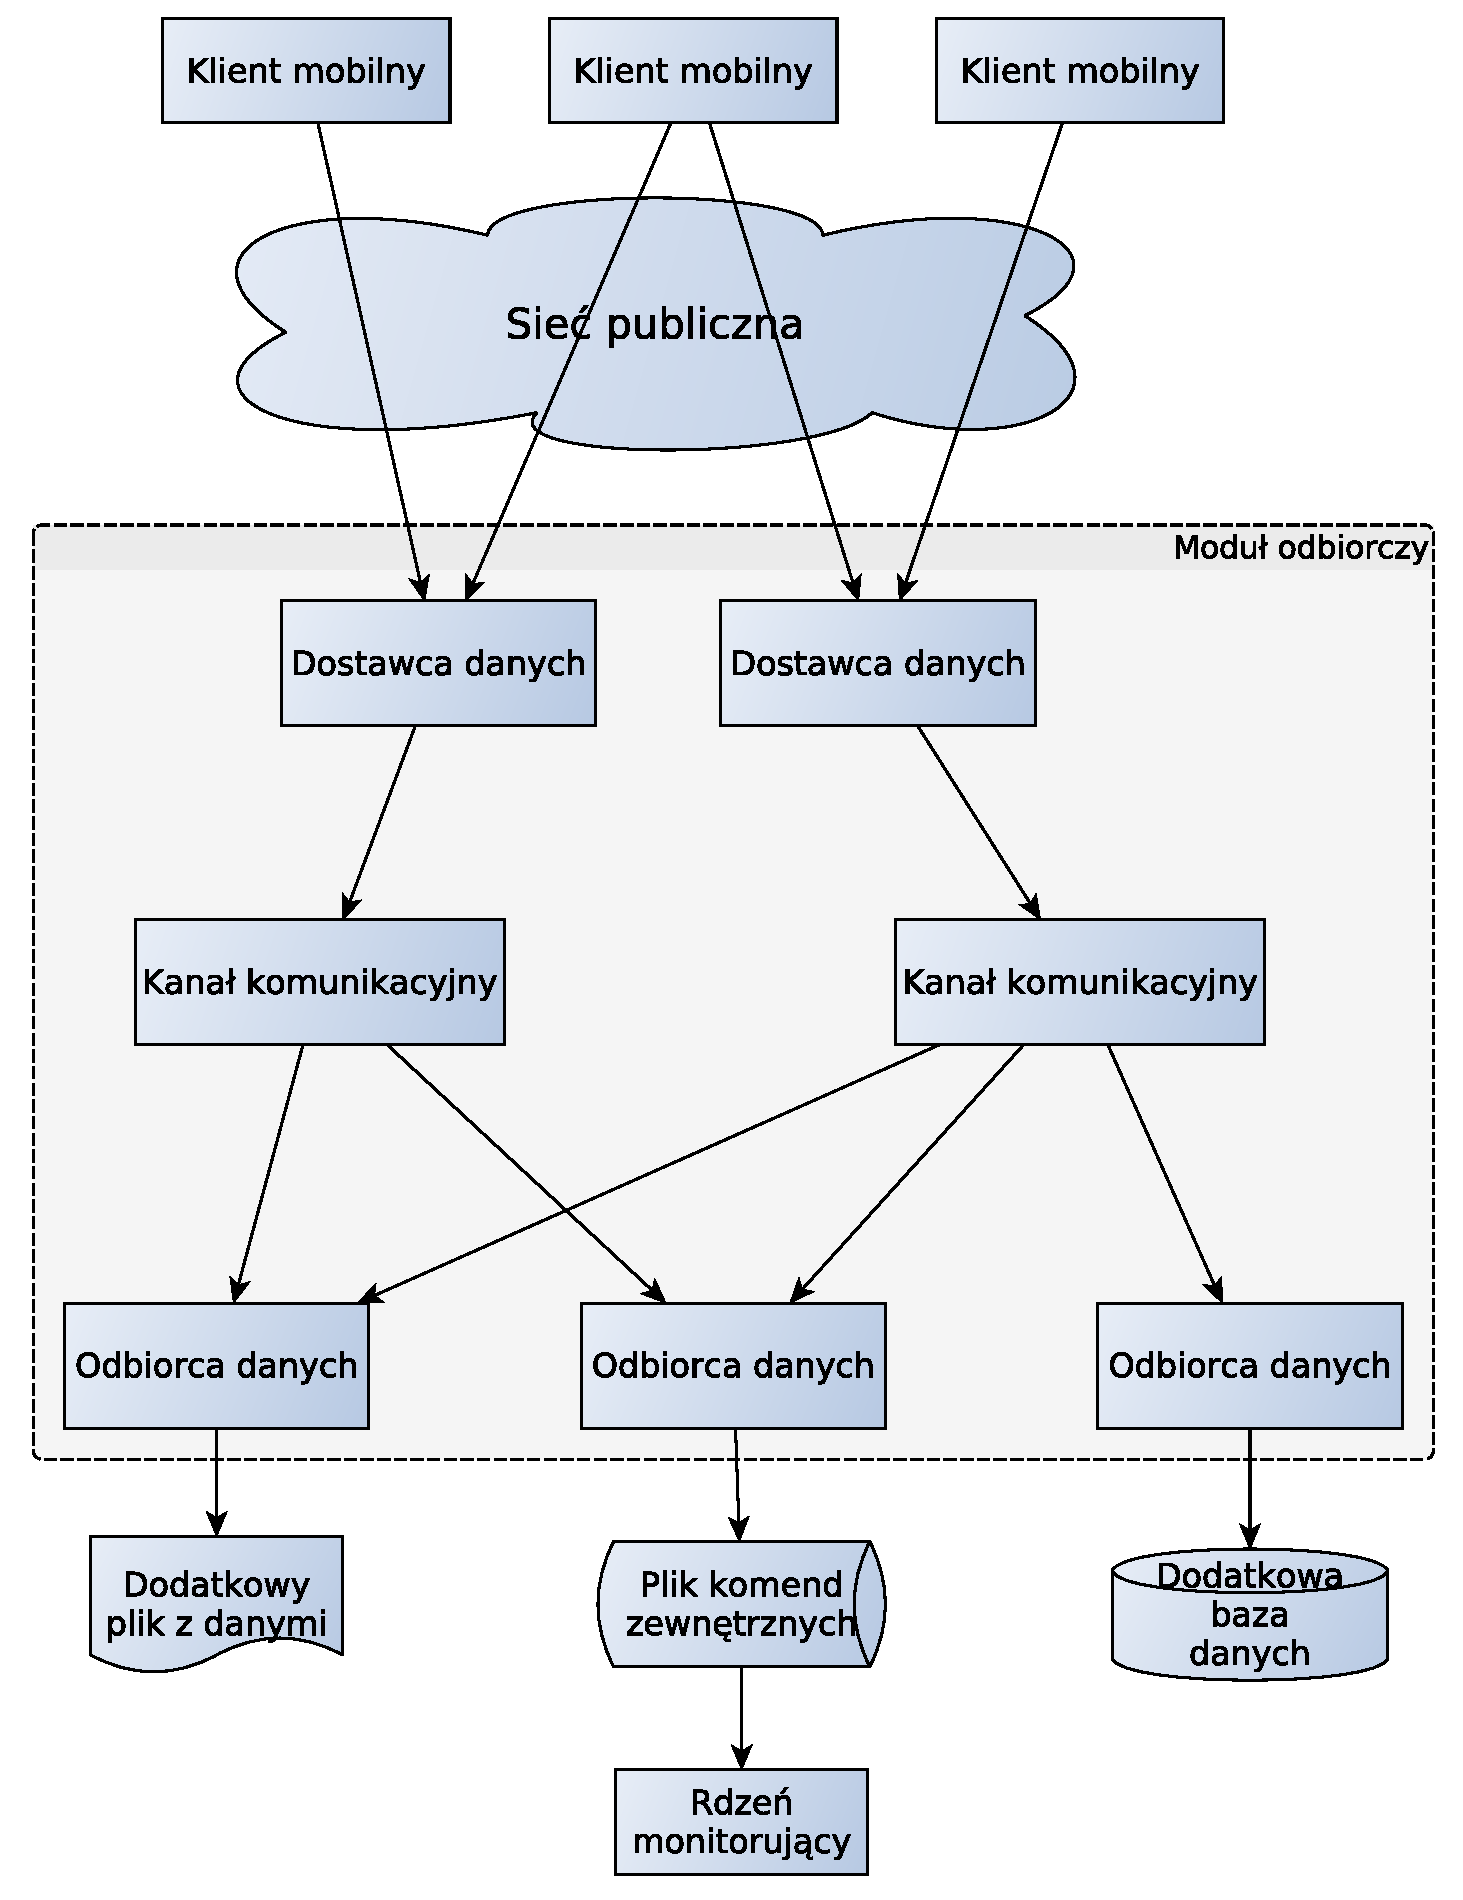
\includegraphics[width=0.7\textwidth]{img/odbiorczy}
\end{figure}

Wymagania przedstawione w~\ref{chap:Wymagania} wymuszają umożliwienie
dodawania nowych algorytmów zarówno kryptograficznych jak i~algorytmów
uwierzytelnienie klienta. W~celu spełnienia tych wymagań wyróżnione
zostały w!programie również dwa moduły pomocnicze:

\begin{itemize}
\item moduł uwierzytelnienia,
\item moduł kryptograficzny.
\end{itemize}

Moduł uwierzytelnienia stanowi bibliotekę algorytmów uwierzytelnienia
klienta, które mogą być wykorzystane przez dostawców danych w~celu
weryfikacji tożsamości klienta. Moduł kryptograficzny stanowi
natomiast bibliotekę algorytmów kryptografii symetrycznej,
asymetrycznej oraz funkcji skrótu. Umożliwia to realizację procesu
negocjacji algorytmu symetrycznego wykorzystywanego przez protokół
komunikacyjny. Ponieważ różnice pomiędzy poszczególnymi protokołami
komunikacyjnymi mogą być niewielkie w~programie wyodrębniono również
moduł implementujący poszczególne warstwy protokołu. Umożliwi to w
przyszłości szybką modyfikację protokołu komunikacyjnego lub dodanie
nowego.


\chapter{Implementacja}
\label{chap:Implementacja}

W rozdziale \ref{chap:ProjektSystemu} przedstawiono autorskie
rozwiązanie problemu monitorowania klienta mobilnego przy uzyciu
systemu Icinga. W ramach projektowania takiego systemu dokonano
analizy dostępnych na rynku dodatków pod kątem ich przydatności w
systemie monitorowania klienta mobilnego. Przeprowadzona analiza
wykazała konieczność opracowania nowego dodatku, pozwalającego na
przekazywanie w sposób zgodny z wymaganiami, danych z urządzenia
mobilnego do serwera.  Dodatek ten --- NSCAv2 został zaprojektowany i
zaimplementowany w ramach niniejszej pracy. Rozdział ten zawiera
dokładny opis funkcjonalny tego dodatku oraz przedstawia istotne
elementy implementacji tego dodatku.

Ponadto w proponowanym systemie występuje aplikacja przeznaczona dla
platformy mobilnej. Implementacja takiej aplikacji wykracza poza
zakres tej pracy.  W ramach serii prac dyplomowych przygotowywanych na
Wydziale Elektroniki i Technik Informacyjnych powstała również praca
inżynierska Pana Marcina Kubika. Przedmiotem tej pracy jest projekt
oraz implementacja dla platformy Android aplikacji
IcingaMini. Pobierzny opis koncepcji i potrzeby tej aplikacji mozna
znaleźć w~\ref{sec:IcingaMini} natomaist szczegółowy opis
implementacji został zawarty w~\cite{book:pracaKubika}.

\section[Opis architektury][Opis architektury]{Opis architektury}


Konceptualny model dodatku został przedstawiony
w~\ref{sec:ProjModOdb}. Fizyczna struktura programu jest dużo bardziej
złożona. Została utworzona z~użyciem biblioteki Qt jako podstawowego
szkieletu aplikacji. Wykorzystano również biblioteki boost oraz
Crypto++. Dodatek ten przeznaczony jest, podobnie jak system
monitorujący Icinga dla komputerów pracujących pod kontrolą systemu
operacyjnego Linux i~jest uruchamiany jako samodzielny
serwis. Fizyczna struktura programu składa się z~następujących
elementów:

\begin{description}
\item[Szkielet programu] --- Zawiera on elementy programu, konieczne do
  wytworzenia środowiska dla funkcjonowania pozostałych modułów oraz
  zarządzania nimi. Ponadto zawiera odwzorowanie bytów logicznych
  (dostawca, konsument, kanał komunikacyjny) programu w strukturę
  fizyczną.
\item[Moduł kryptograficzny] --- Dostarcza on implementacji funkcji
  kryptograficznych, wymaganych podczas komunikacji z klientem
  mobilnym. Zawiera on zarówno algorytmy asymetryczne, konieczne do
  inicjalizacji kryptografii symetrycznej, jak i~algorytmy symetryczne,
  służące do przesyłania danych.
\item[Moduł autoryzacji klienta] --- Zawiera on implementację algorytmów
  uwierzytelnienia klienta.
\item[Moduł komunikacji z użyciem TCP] --- Dostarcza on implementację
  protokołu komunikacyjnego używanego do komunikacji z~klientem.
\item[Moduł logowania] --- Pozwala na przekazywanie użytkownikowi
  komunikatów z~dowolnych miejsc znajdujących się w~innych
  modułach. Wiadomość ta może zawierać informacje o~zaistniałym
  błędzie, lub innym zdarzeniu wymagającym poinformowania użytkownika.
\end{description}

%rysunek o wspolpracy tych elementow

Odwzorowanie podstawowych elementów struktury logicznej w~fizyczną ma
miejsce w~szkielecie aplikacji. Pozostałe elementy programu zostały
zaprojektowane jako moduły pomocnicze świadczące dobrze zdefiniowane
usługi. Szczególnym przykładem, tego usługowego charakteru pozostałych
modułów, może być moduł kryptograficzny i~moduł autoryzacji
klienta. Udostępniają one generyczne interfejsy dostępu do swoich
usług dla pozostałych modułów. Szczegóły implementacyjne są natomiast
zamknięte wewnątrz modułów. Typ faktyczny obiektu udostępnianego
poprzez generyczny interfejs jest w~bardzo wielu przypadkach
determinowany dopiero na etapie konfiguracji programu. Ponadto liczba
klas znajdujących się w~tych modułach może znacząco rosnąć. Jednym z
wymagań było zapewnienie możliwości definiowania nowych algorytmów
kryptograficznych jak i~algorytmów uwierzytelnienia klienta. W~celu
zapewnienia możliwości wybrania typu faktycznego obiektu na podstawie
danych wykorzystano wzorzec projektowy fabryki\footnote{Wzorzec ten
  został szczegółowo opisany w~\cite[101-109]{book:wzorce}.}.  Każdy
z~wspomnianych modułów posiada swojego zarządcę (fabrykę). Dostępne
w~module obiekty muszą zostać zarejestrowane u~swojego
zarządcy. Pozostałe moduły uzyskują instancje tych obiektów, poprzez
zarządcę, który na podstawie przekazanych danych określa typ faktyczny
obiektu. Jeśli dany typ jest dostępny, zostanie on wówczas przekazany
wywołującemu i~będzie on mógł używać go poprzez dostarczony generyczny
interfejs. Logiczna struktura tych modułów wymaga zapewnienia, że
w~programie istnieje tylko jedna instancja obiektu danego
zarządcy. W~tym celu został wykorzystany wzorzec projektowy
singleton\footnote{Szczegółowe omówienie wzorca singleton można
  znaleźć w~\cite[130-138]{book:wzorce}.}. Zastosowanie wzorca
projektowego fabryki pozwala pozostałym modułom, na korzystanie z
obiektów, których typ faktyczny jest nieznany w~trakcie implementacji
oraz kompilacji programu.

W~celu konfiguracji programu wykorzystano zewnętrzny plik w~formacie
XML. Umożliwia to zmianę ustawień programu bez konieczności jego
ponownej kompilacji. Plik konfiguracyjny składa się z~czterech
zasadniczych sekcji:

\begin{description}
\item[Sekcja dostawców danych] zawiera dane dostawców, którzy mają
  zostać uruchomieni podczas startu programu. Umożliwia przekazanie
  dodatkowych informacji do obiektu dostawcy np. adresu IP lub portu
  na którym powinien on oczekiwać na połączenia. 
\item[Sekcja odbiorców danych] zawiera dane odbiorców danych, którzy
  mają zostać uruchomieni podczas startu programu. Umożliwia
  przekazanie dodatkowych informacji do obiektu odbiorcy danych,
  takich jak ścieżka do pliku do którego należy zapisywać dane. 
\item[Sekcja definicji klientów] zawiera definicję klientów oraz grup
  klientów. Każda definicja klienta składa się z następujących sekcji:
  \begin{description}
  \item[Sekcja autoryzacji] zawiera dane o dozwolonych modułach
    autoryzacyjnych dla danego klienta. Umożliwia także dodatkową
    konfigurację instancji modułów przeznaczonych dla danego klienta.
  \item[Sekcja filtrowania] zawiera urządzenia oraz usługi, których
    dane monitorowania mogą być przesyłane przez tego konkretnego
    klienta.
  \end{description}
\item[Sekcja definicji ścieżek danych] zawiera definicję ścieżek
  danych w~programie. Pozwala na definiowanie, do którego odbiorcy
  danych mają trafić dane odebrane od wskazanego klienta.
\end{description}

Podczas uruchamiania programu, plik konfiguracyjny zostaje przeczytany
oraz sprawdzony pod kątem poprawności zarówno składniowej jak
i~semantycznej. Obiekty dostawców, odbiorców oraz algorytmów
uwierzytelnienia dostarczane są przez zewnętrznych programistów, zatem
prawidłowość ich ustawień nie może być sprawdzana na tym samym
etapie. Jest to wykonywane dopiero w~trakcie inicjalizacji danego
obiektu. Należy zatem zawsze po pomyślnej analizie pliku
konfiguracyjnego sprawdzić zawartość pliku dziennika wykonania
programu. 

Definicje klientów znajdujące się w pliku konfiguracyjnym są nie
zbędne dla zapewnienia bezpieczeństwa całego systemu. Dodatek NSCAv2
pozwoli na komunikację z klientem, tylko jeśli został on zdefiniowany
w konfiguracji. Według wymagań konieczne jest zapewnienie
niezależności algorytmów uwierzytelnienia klienta od pozostałych
elementów. Definicja każdego klienta zawiera zatem listę modułów
uwierzytelnienia, których dany klient moze używać. Program zapewnia
równiez kontrolę przesyłanych danych zatem konieczne jest określenie
listy dozwolonych urządzeń i usług, o których dany klient moze
przesyłać informacje.

Jednym z wielu wymagań stawianych na etapie projektowania systemu było
zapewnienie mozliwości przekazywania danych pochodzących od klinta
mobilnego do wielu miejsc docolewych, takich jak systemy monitorujące
czy bazy danych. Polityka dostarczania danych jest zdecydowanie
elementem konfiguracyjnym i nie powinna być ona zaszyta w
implementacji programu. W wykonanym programie logika przekazywania
danych definiowana jest w programie poprzez sekcję definicji ścieżek
danych. Sekcja ta pozwala na definiowanie w jakie miejsca powinny
zostać przekazane dane na podstawie klienta, który te dane przysłał
oraz dostawcy, który te dane odebrał.

Przeniesienie znacznej cześci logiki programu do pliku
konfiguracyjnego maiało znaczący wpływ na architekturę
rozwiązania. Program stanowi jedynie zbiór elementów, z których przy
pomocy pliku konfiguracyjnego składa się w pełni funkcjonalny dodatek.

\section[Szkielet programu][Szkielet programu]{Szkielet programu}

Moduł ten zawiera podstawowe komponenty programu. Zawarto tutaj
wszystkie czynności przygotowawcze związane z~wczytaniem konfiguracji
oraz utworzeniem obiektów z~niej wynikających. Ponadto w~module tym
znajdują się definicję podstawowych bytów logicznych
programu. W~zależności od pełnionej funkcji można wyróżnić następujące
grupy obiektów:

\begin{description}
\item[Grupa obiektów konfiguracyjnych] zawiera wszystkie obiekty
  używane zarówno do wczytania parametrów uruchomienia programu
  z~linii poleceń, jak również obiekty odpowiedzialne za dostarczenie
  do programu konfiguracji zawartej w pliku.
\item[Grupa obiektów producentów danych] \raggedright{zawiera generyczny interfejs
  producenta danych oraz fabrykę, umożliwiającą pozyskiwanie obiektów
  z~tej grupy, a~także definicję dostępnych producentów danych.}
\item[Grupa obiektów konsumentów danych] zawiera generyczny interfejs
  konsumenta danych oraz fabrykę, umożliwiającą pozyskiwanie obiektów
  z~tej grupy, a~także definicję dostępnych konsumentów danych.
\item[Grupa obiektów filtrujących] zawiera obiekty pozwalające na
  kontrolę danych otrzymywanych od klienta
\item[Grupa obiektów kanału komunikacyjnego] zawiera obiekty powiązane
  z~kanałem komunikacyjnym pomiędzy producentami danych, a~ich
  konsumentami. Zawiera również mechanizmy formatowania danych oraz
  bufory przeznaczone na dane oczekujące na przekazanie.
\item[Grupa obiektów zarządzających] zawiera zarządcę programu oraz
  obiekty pomocnicze. Wykonywane są tutaj wszelkie czynności, które
  należy wykonać w~trakcie uruchamiania programu, a~także tworzenie
  oraz niszczenie obiektów implementujących elementy logiczne
  programu.
\end{description}

\subsubsection[Grupa obiektów konfiguracyjnych][Grupa obiektów
konfiguracyjnych]{Grupa obiektów konfiguracyjnych}

Głównym członkiem grupy obiektów konfiguracyjnych jest parser pliku
konfiguracyjnego. Ponieważ plik konfiguracyjny posiada strukturę pliku
XML możliwe było wykorzystanie czytelnika strumienia XML z~biblioteki
Qt. Klasa ta zapewnia generację znaczników oraz sprawdzanie
poprawności składniowej czytanego dokumentu. Umożliwiło to
implementację prostego parsera rekursywnie zstępującego, który zajmuje
się jedynie sprawdzaniem poprawności logicznej znaczników. Ze względu
na strukturę plików XML, nie jest możliwa pełna bieżąca kontrola
danych w~nim zawartych. Konieczne jest zatem wczytanie pliku
konfiguracyjnego i~odwzorowanie go w~strukturach danych, a~następnie
wykonanie sprawdzenia spójności oraz poprawności tych danych. Obiekt
parsera konfiguracji jest również globalnym obiektem udostępniającym
parametry konfiguracji. W~obiekcie tym znajdują się wszystkie
ustawienia oraz definicje wszystkich obiektów logicznych programu.

\subsubsection[Grupa obiektów producentów danych][Grupa obiektów
producentów danych]{Grupa obiektów producentów danych}

Grupa obiektów producentów danych składa się z~dwóch głównych
elementów. Pierwszym z~nich jest klasa implementująca wzorzec
fabryki. Pozwala ona pozostałym obiektom na uzyskiwanie instancji
obiektu dostawcy danych, bez konieczności znania jego typu faktycznego
w~trakcie pisania kodu czy też kompilacji. Drugim z~elementów jest
generyczny interfejs dostawcy danych, który musi być implementowany
przez każdego dostawcę. Interfejs ten jest bardzo prosty jednak
pozwala na wykonywanie wszystkich niezbędnych operacji.

Każdy dostawca danych powinien dostarczyć implementacji dwóch
funkcji. Funkcja {\em initImpl()} jest wywoływana z funkcji {\em
  init()} w chwili inicjalizacji konkretnego obiektu klasy parametrami
pochodzącymi z pliku konfiguracyjnego. Pozwala to między innymi na
przekazanie dodatkowych danych inicjujących takich jak adres sieciowy
czy numer portu. Dostawca danych powinien w funkcji {\em initImpl()}
pobrać wszystkie niezbędne mu dane z dostarczonych parametrów, a
następnie wykonać wszystkie czynnosci przygotowawcze takie jak
uruchomienie dodatkowego wątku. Po wyjściu z tej funkcji z sukcesem
przyjmuje się, ze dostawca został zainicjalizowany poprawnymi danymi
oraz jest on uruchomiony i oczekuje na dane od klientów. Istotne jest
również dostarczenie implementacji funkcji {\em close()}. Jest ona
odpowiedzialna za zakończenie pracy tego dostawcy danych i zwolnienie
wszystkich używanych przez niego zasobów.

%interfejs dostawcy danych

Należy również nadmienić, że konieczne było również dostarczenie
odpowiedniego mechanizmu rejestracji definiowanych obiektów
w~fabryce. Istotne jest, aby umożliwić programiście rejestrację nowego
typu faktycznego obiektu bez konieczności ingerencji w~inne pliki
źródłowe. W~celu ułatwienia tego procesu zostało opracowane makro,
które dzięki wykorzystaniu szablonów dokonuje automatycznej
rejestracji nowego typu faktycznego obiektu w~fabryce. Dzięki jego
wykorzystaniu programista, podczas dodawania nowego dostawcy danych,
musi zapewnić jedynie deklarację oraz definicję nowego typu. Warto
zauważyć, że sposób implementacji tego makra pozwala na umieszczenie
definicji nowego typu w~pliku nagłówkowym, który jest włączany do
wielu jednostek translacji i nie powoduje to błędów kompilacji ani
błędów funkcjonowania procesu rejestracji.

\vspace{0.5cm}
\begin{minipage}{\textwidth}
\begin{lstlisting}[language=c++, caption=Definicja dostawcy danych, linewidth=10cm]
DATA_PROVIDER(NazwaTypu, NazwaRejestrowana)
{
  //deklaracja metod
}
\end{lstlisting}
\end{minipage}
\vspace{0.5cm}

W~ramach tej grupy obiektów dostarczono również referencyjną
implementację dostawcy o~nazwie typu {\em DefaultTcpProvider}. Stanowi
on implementację omówionego wcześniej protokółu
komunikacyjnego. W~celu zapewnienia lepszej wydajności, logika
funkcjonowania tego dostawcy została przeniesiona do osobnego wątku
programu. Aby zapewnić elastyczności wykorzystania tego obiektu
możliwe jest definiowanie z~poziomu pliku konfiguracyjnego zarówno
adresu IP i~portu wykorzystywanego przez ten obiekt, a~także wskazanie
pliku zawierającego klucz prywatny.

\subsubsection[Grupa obiektów konsumentów danych][Grupa obiektów
konsumentów danych]{Grupa obiektów konsumentów danych}

Grupa obiektów konsumentów danych posiada analogiczną budowę jak grupa
producentów danych. Zapewnia ona zarówno fabrykę konsumentów danych
jak i~generyczny interfejs konsumenta. Interfejs konsumenta danych
jest analogiczny jak dla dostawcy. Rejestracja obiektów w~fabryce
odbywa się również przy użyciu analogicznego makra. W~ramach tej grupy
obiektów dostarczono implementację dwóch konsumentów danych. Pierwszy
z~nich o~nazwie typu {\em ToScreenPrinter}, spełnia jedynie funkcję
kontrolną. Wszystkie dane, które do niego trafią są natychmiast
wypisywane w~dzienniku wykonania programu. Dostawca typu {\em
  ToIcingaWriter} odpowiedzialny jest natomiast za przekazywanie
wszystkich danych do pliku komend zewnętrznych systemu Icinga. Możliwa
jest zmiana ścieżki pliku komend zewnętrznych systemu Icinga poprzez
plik konfiguracyjny.

\subsubsection[Grupa obiektów filtracji][Grupa obiektów
filtracji]{Grupa obiektów filtracji}

Grupa obiektów filtracji pozwala na kontrolę danych otrzymywanych od
klienta, a także na pobierani informacji o danym kliencie. Podstawowym
elementej tej grupy jest fizyczne odwzorowanie bytu klienta w
odpowiednią klasę. Pozwala to na uzyskiwanie przez inne moduły w
prosty sposób wszystkich niezbędnych infrormacji na temat
obsługiwanego klienta. Każdy klient posiada zdefiniowany w~pliku
konfiguracyjnym zbiór urządzeń i~usług, o~których informacje może
przesyłać. Obiekty z~tej grupy, które są odpowiedzialne za kontrolę
odbieranych danych, pobierają z~analizatora składniowego wspomniane
zbiory i~dokonują kontroli każdego wpisu dziennika otrzymanego od
klienta. Jeśli klienta nadesłał dane dotyczące urządzenia lub usługi,
do których nie ma on uprawnień, nie będzie możliwe przekazanie ich do
konsumentów.

\subsubsection[Grupa obiektów kanału komunikacyjnego][Grupa obiektów
kanału komunikacyjnego]{Grupa obiektów kanału komunikacyjnego}

Grupa obiektów kanału komunikacyjnego odpowiedzialna jest za
niezawodne przekazanie danych od dostawcy danych do konsumentów według
reguł zdefiniowanych w~pliku konfiguracyjnym. Zapewnienie
niezawodności zostało osiągnięte poprzez implementację bufora kołowego
wewnątrz pliku. Każdy dostawca danych posiada swój plik bufora. Na
początku tego pliku zapisane są położenia miejsca przeznaczonego do
czytania oraz miejsca przeznaczonego do pisania. Dane, które logicznie
znajdują się pomiędzy miejscem do czytania, a~miejscem do pisania są
to dane, które zostały odebrane od klienta lecz nie zostały jeszcze
dostarczone do konsumentów. Pomyślnie zweryfikowana przez obiekty
filtrujące porcja danych przekazywana jest z~użyciem kanału
komunikacyjnego do konsumentów danych. Operacja ta odbywa się w~dwóch
etapach. Pierwszy etap dokonuje zapisu danych do pliku bufora. Jeśli
aktualnie nie ma żadnych danych oczekujących na przetworzenie przez
konsumentów, nowa porcja danych jest niezwłocznie dostarczana do
odpowiednich obiektów. Jeśli istnieją porcje danych, które oczekują na
zapisanie dane zostaną zapisane do pliku i~dostarczone, po danych,
które nadeszły przed nimi. Należy zwrócić uwagę, że dane zapisywane są
na dysku tylko raz, niezależnie od liczby konsumentów do których
powinny one zostać dostarczone. Ponadto dostawca danych uzyskuje
potwierdzenie zapisania danych po zakończeniu pierwszego etapu ich
obługi czyli już po zapisaniu do pliku bufora. Oznacza to, że dostawcy
danych są w~znacznym stopniu niezależni od konsumentów danych. Pozwala
to skrócić do minimum czas oczekiwania klienta mobilnego pomiędzy
wysłaniem danych, a~uzyskaniem potwierdzenia o~ich przetworzeniu.

\subsubsection[Grupa obiektów zarządzających][Grupa obiektów
zarządzających]{Grupa obiektów zarządzających}

Głównym przedstawicielem grupy obiektów zarządzających jest klasa
główna programu. Program został napisany zgodnie z~metodyką obiektową
zatem cała logika wykonania programu została również zamknięta
w~klasie co uprościło funkcję główną programu do minimum. Klasa ta
odpowiedzialna jest za przebieg całości programu. Pierwszą operacją
wykonywaną przez tą klasę jest odnalezienie pliku konfiguracyjnego
i~zlecenie jego wczytania przez parser konfiguracji. Na podstawie
informacji uzyskanych w~wyniku analizy pliku konfiguracyjnego klasa
główna programu pobiera z~odpowiednich fabryk wszystkie obiekty
producentów oraz konsumentów zdefiniowanych w~pliku
konfiguracyjnym. Po uzyskaniu obiektów następuje ich inicjalizacja na
podstawie danych wczytanych z pliku konfiguracyjnego. Klasa ta jest
również odpowiedzialna za prawidłową deinicjalizację oraz destrukcję
wszystkich obiektów. Ponadto należy zauważyć, że omawiany program
funkcjonuje jako serwis systemowy, zatem konieczne jest również
wykonanie w~tej klasie wszystkich czynności zalecanych przy
uruchamianiu takich serwisów. Całość programu została napisane zgodnie
z~paradygmatem zdarzeniowym. Oznacza to, że po wykonaniu inicjalizacji
program zawiesza swoje wykonanie do czasu otrzymania jakiegoś
zdarzenia, na które powinien on zareagować. Użycie biblioteki Qt w
znaczny sposób uprościło oczekiwanie na zdarzenia dzięki mozliwości
użycia pętli zdarzeń z tej biblioteki.

\section[Moduł kryptograficzny][Moduł kryptograficzny]{Moduł kryptograficzny}

Moduł ten dostarcza pozostałym elementom programu implementacji
algorytmów kryptograficznych. Dostępne są generyczne interfejsy do
następujących schematów algorytmów:

\begin{itemize}
\item szyfrowanie symetrycznych,
\item szyfrowanie asymetrycznych,
\item funkcja skrótu,
\item podpis cyfrowy.
\end{itemize}

%definicje interfejsów kryptograficznych

Definicje wszystkich interfejsów zostały przedstawione na
rys.~\ref{fig:cryptoInterface}. Dostarczanie implementacji danego
schematu kryptograficznego odbywa się w~sposób analogiczny do
dostarczania implementacji dostawców danych. Wszystkie implementacje
algorytmów zostają zarejestrowane w~fabryce kryptograficznej, która
umożliwia uzyskiwanie obiektu o~typie określanym na podstawie danych,
na przykład odebranych od klienta.

% biblio do CBC i AESA
W~ramach tej pracy dostarczono kilku algorytmów, które były konieczne
do zaimplementowania protokołu komunikacyjnego. Jako algorytm
symetryczny dostarczona została implementacja algorytmu AES
pracującego w~trybie wiązania bloków zaszyfrowanych. Omawiany tryb
pracy algorytmu powoduje powstanie zależności pomiędzy kolejnymi
blokami. Oznacza to, że manipulacja jednym blokiem powoduje zmiany
wartości odszyfrowanych w~tym bloku i~każdym następnym. Zastosowanie
tego trybu w~implementowanym protokole komunikacyjnym pozwala na
zagwarantowanie, że sekwencja wiadomości otrzymywanych od klienta nie
została zmieniona\footnote{Samo wykorzystanie trybu CBC nie daje
  gwarancji ale w protokole komunikacyjnym użyto również
  funkcji skrótu, przez co możliwe jest jej udzielenie.}. Protokół
komunikacyjny wymagał również dostarczenia asymetrycznego algorytmu
RSA. W~module zdefiniowano ponadto klasę implementującą generyczny
interfejs funkcji skrótu, która dostarcza funkcjonalności algorytmu
SHA-2 o~długości skrótu 256 bitów. Jeden z~etapów protokołu
komunikacyjnego wymagał również dostarczenia algorytmu podpisu
cyfrowego opartego na algorytmie RSA.

Do implementacji wszystkich algorytmów została wykorzystana biblioteka
Crypto++. Jest to popularna biblioteka o~otwartych źródłach napisana
w~języku~C++, która w~obiektowy sposób udostępnia algorytmy
kryptograficzne.

\section[Moduł uwierzytelnienia][Moduł uwierzytelnienia klienta]{Moduł uwierzytelnienia klienta}

Moduł posiada architekturę typową dla modułów usługowych. Głównym
elementem jest klasa implementująca wzorzec fabryki oraz generyczny
interfejs pozwalający na wykorzystywanie obiektów uzyskanych
z~fabryki.

Interfejs zdefiniowany dla algorytmów uwierzytelnienia został
zaprojektowany z~wykorzystaniem mechanizmu sygnałów i~slotów
z~biblioteki Qt. Użycie tego mechanizmu pozwala na znacznie bardziej
wydajne wykorzystanie zasobów. Przykładem takiej optymalizacji może
być czas gdy klient przetwarza żądanie związanie z~uwierzytelnieniem
wątek serwera nie musi być wtedy bezczynny lecz może przetwarzać
żądania pochodzące od innych klientów. Definicja interfejsu pozwala
również na przekazanie do niego dodatkowych ustawień pochodzących
z~pliku konfiguracyjnego. Każdy algorytm uwierzytelnienia powinien po
zakończeniu sukcesem lub porażką procesu uwierzytelnienia klienta
wykonać emisję sygnału z~interfejsu algorytmu wraz z~rezultatem
procesu autoryzacji. Ponieważ z~punktu widzenia protokołu istotne jest
przekazanie danych autoryzacyjnych jako informacja o~akceptacji
algorytmu uwierzytelnienia, konieczne jest aby każdy algorytm przesłał
co najmniej jedną wiadomość do klienta.

Zapewnienie niezależności implementacji algorytmów uwierzytelnienia od
wykorzystywanej aktualnie metody komunikacji wymagało zdefiniowania
generycznego interfejsu komunikacyjnego, który może być wykorzystywany
przez implementacje poszczególnych algorytmów. Implementacja tego
interfejsu powinna być dostarczona przez moduł, który jest aktualnie
wykorzystywany w~programie do komunikacji z~klientem.

%sekwencja uwierzytelnienie

Przykładowy przebieg procesu uwierzytelnienia został przedstawiony na
rys.~\ref{fig:sekwencjaAuth}. Proces ten rozpoczyna się od ustawienia
aktualnie wykorzystywanego interfejsu komunikacyjnego. Następnie
wykonywane jest rozpoczęcie procesu uwierzytelnienia. W ramach tego
procesu moduł uwierzytelnienia moze komunikować się z klientem poprzez
otrzymany wcześniej obiekt. Po zakończeniu procesu autoryzacji
emitowany jest odpowiedni sygnał informujący pozostałe komponenty o
rezultacie uwierzytelnienia.

W~ramach pracy został zaimplementowany również przykłądowy moduł
uwierzytelnienia klienta. Nosi on nazwię: {\em LoginPass}. Jest to
prosta metoda uwierzytelnienia oparta na pobraniu od klienta loginu
oraz hasła i~porównanie go z~danymi dostarczonymi w~pliku
konfiguracyjnym. Każdy klient posiada w~pliku konfiguracyjnym listę
dostępnych dla niego algorytmów uwierzytelnienia wraz z~danymi jakie
powinny być przekazane, aby zapewnić pozytywne wykonanie
procesu. Należy zwrócić uwagę, że zaimplementowany algorytmy
uwierzytelnienia stanowi jedynie przykład, w jaki sposób powinno się
definiować algorytmy w opracowanym dodatku. Ich wykorzystanie w
systemie produkcyjnym zależy od bezpieczeństwa serwera, na którym
znajduje się program NSCAv2. Należy być świadomym, że wszystkie hasła
oraz nazwy użytkowników przechowywane są jawnym tekstem w~pliku
konfiguracyjnym\footnote{Sposób przechowywania loginu oraz hasła na
  urządzeniu mobilnym jest uzależnione od konkretnej implementacji
  aplikacji IcingaMini.}. Nie stanowi to oczywiście zagrożenia jeśli
do serwera monitorujacego dostęp mają jedynie uprzywilejowane
osoby. Należy przypomnieć, że na sewerze znajdują się również klucze
prywatne RSA, więc zawsze nalezy zwrócić szczególną uwagę, na
bezpieczeństwo serwera.

\section[Moduł TCP][Moduł komunikacji z wykorzystaniem TCP]{Moduł komunikacji z wykorzystaniem TCP}

Moduł ten zawiera implementację protokołu komunikacyjnego opisanego
w~rozdziale~\ref{sec:ProtKom}. Inicjacja każdej z~warstw protokołu
została zaimplementowana w~dedykowanej klasie lub jeśli proces
inicjacji złożony był z~kilku rozdzielnych logicznie elementów, każdy
element został zaimplementowany w~osobnej klasie. W~celu umożliwienia
każdej z~warstw protokołu korzystanie z~usług warstw niższych w~sposób
generyczny wykorzystany został wzorzec dekoratora.

Aby wykorzystać wzorzec dekoratora zdefiniowano generyczny interfejs
pozwalający na odczytanie oraz zapisanie komunikatu niezależnie od
liczby warstw znajdujących się poniżej. Klasą prostą w tym przypadku
jest prosta klasa opakowująca gniazdo TCP z biblioteki Qt. Klasami
dekorującymi są klasy odpowiadające za kolejne czynności w wyższych
warstwach protokołu. Klasy te są odpowiedzialne, za formowanie
wiadomości, szyfrowanie oraz obliczanie i kontrolę jej
skrótu. Ponieważ kolejność czynności wykonywanych w trakcie budowania
wiadomości jest istotna zastosowano rekurencyjne budowanie
wiadomości. Każda klasa dekoratora posiada jedynie jedno wskazanie do
obiektu, który znajduje się o poziom niżej w hierarchii. Użytkownik
zapisuje wiadomość używając klasy z najwyższej warstwy. Obiekt
tendokonuje przekształcenia wiadomości zgodnie ze swoim algorytmem, a
następnie wywołuje tą samą metodę na rzecz obiektu znajdującego się o
jeden nizej w hierarchii niż ona sama przekazując przekształconą
wiadomość jako parametr wywołania.

%diagram z tymi klasami

Wykorzystanie wzorca dekoratora pozwoli w~przyszłości na łatwą
modyfikację protokołu komunikacyjnego np. poprzez dodanie dodatkowej
warstwy. Ponadto wprowadzenie jednolitego interfejsu pozwoliło na
zachowanie prostoty i~jednolitości implementacji poszczególnych warstw
protokołu komunikacyjnego.

Moduł ten został zaimplementowaniu przy użyciu licznych mechanizmów
z~biblioteki Qt. Przede wszystkim wykorzystany został moduł sieciowy
wspomnianej biblioteki. Dzięki jego użyciu uzyskano dostęp do
generycznej implementacji serwera TCP, a~także gniazd. Szkielet
aplikacji Qt pozwolił na wygodną implementację asynchronicznej
komunikacji z~użyciem gniazd TCP przy pomocy standardowego dla tego
szkieletu mechanizmu sygnałów i~slotów. Dzięki temu uzyskano
przejrzysty i~wydajny kod, który pozwala na obsługę wielu klientów
w~jednym wątku.

\section[Moduł logowania][Moduł logowania]{Moduł logowania}

Omawiany dodatek wykonywany jest bez interakcji
z~użytkownikiem. Funkcjonuje on jako serwis systemowy. Docelowo będzie
on wykonywany na serwerze, poza sesją jakiegokolwiek
użytkownika. W~trakcie wykonania programu mogą się zdarzyć sytuacje
wymagające poinformowania użytkownika o~ich wystąpieniu. Znaczna część
z~tych informacji stanowi jedynie zapis wykonania programu, jednak
mogą występować również informacje o sytuacjach krytycznych, o których
użytkownik musi zostać powiadomiony. Konieczne było zatem dostarczenie
możliwości przekazywania takich informacji z~wielu modułów do jednego,
wspólnego miejsca, które stanowi dziennik wykonania serwisu.

Każdy moduł posiada możliwość przekazywania użytkownikowi wiadomości
o~różnym priorytecie. Dozwolone są następujące priorytety:

\begin{description}
\item[FATAL] najwyższy priorytet, wiadomość zawiera komunikat
  o~błędzie, który uniemożliwia dalsze wykonanie programu
\item[ERROR] komunikat zawiera informacje o~błędzie, który
  uniemożliwia wykonanie pewnej ścieżki programu
\item[WARNING] komunikat zawiera ostrzeżenie o~nietypowej sytuacji
\item[DEBUG] komunikat zawiera treść pomocną podczas wyszukiwania błędów
\item[INFO] komunikat zawiera jedynie treści informacyjne
\end{description}

Podczas kompilacji ustalany jest minimalny priorytet wiadomości, które
mają być przekazywane użytkownikowi. Wszystkie wiadomości
o~priorytecie niższym niż ustalony, nie zostaną zapisane. Ponadto
dzięki użyciu mechanizmów opartych o~szablony wszystkie komunikaty
o~priorytecie niższym zostaną rozwinięte do wywołania funkcji
pustej. Wywołanie takie zostanie z bardzo dużym prawdopodobieństwem
zoptymalizowane przez kompilator.

Przekazanie użytkownikowi treści komunikatu w~wielu sytuacjach może
nieść zbyt mało informacji. W~celu umożliwienia przekazania
dodatkowych informacji bez konieczności pisania nadmiernej liczby
komend przy każdym komunikacie, opracowana została makrodefinicja,
która do każdego komunikatu dołączy aktualny stempel czasu, nazwę
pliku w~którym znajduje się komunikat, a~także nazwę funkcji oraz
numer linii. Ponadto komunikat nie musi się składać jedynie z tekstu
lecz można go formować w~taki sam sposób jak pisać do strumienia.

\vspace{0.5cm}
\begin{minipage}{\textwidth}
  \begin{lstlisting}[language=c++, breaklines=true,
    linewidth=0.99\textwidth, caption=Przykładowe wypisanie
    komunikatu]

LOG_ENTRY(MyLogger::DEBUG, "komunikat"<<123);

\end{lstlisting}
\end{minipage}
\vspace{0.5cm}

\vspace{0.5cm}
\begin{minipage}{\textwidth}
\begin{lstlisting}[linewidth=0.99\textwidth, caption=Format komunikatu przekazywanego użytkownikowi]

[stempel czasu][poziom][plik][funkcja][linia]:komunikat123

\end{lstlisting}
\end{minipage}
\vspace{0.5cm}

Ponieważ demon nie jest przypisany do żadnego
z~terminali\footnote{Proces przekształcenia w serwis systemowy zakłada
  zamknięcie destryptorów standardowego wejścia, wyjścia oraz wyjścia
  błędów.} nie ma możliwości przekazywania wiadomości na standardowe
wyjście lub wyjście błędów. Konieczne jest zatem utworzenie pliku, do
którego zapisywane będą komunikaty. Należy zwrócić uwagę, że program
jako serwis systemowy uruchomiony będzie ze znacznie ograniczonymi
prawami, aby podnieść poziom bezpieczeństwa serwera. W~związku
z~powyższym jedynym miejscem, co do którego można założyć, że program
będzie miał dostęp jest katalog plików tymczasowych. Każde
uruchomienie programu powoduje zatem utworzenie w~tym katalogu pliku
składającego się z~nazwy programu oraz stempla czasu zawierającego
czas jego uruchomienia.

\chapter{Testowanie wykonanego systemu}
\label{chap:Testy}

Testowanie systemów składających się z~wielu komunikujących się
ze~sobą elementów jest zadaniem bardzo skomplikowanym. Każdy protokół
komunikacyjny stanowi system rozproszony, którego testowanie
i~implementacja jest zadaniem nietrywialnym. Ze względu na
rozproszoność systemu, a~także wpływ czynników zewnętrznych, takich
jak jakość sygnału czy próby ataków, dostarczenie jedynie testów
jednostkowych czy scenariuszowych jest niewystarczające. W~związku
z~powyższym w~ramach tej pracy wykonano testową konfigurację systemu,
która została uruchomiona w~niewielkiej sieci domowej. Pozwoliło to na
uruchomienie kompletnego systemu oraz weryfikację poprawności
implementacji i~zdefiniowanych wymagań.

\section[Opis infrastruktury][Opis infrastruktury testowej]{Opis infrastruktury testowej}

Konfiguracja została wykonana w~mieszkaniu autora w~oparciu
o~istniejącą infrastrukturę sieci lokalnej. Sercem konfiguracji jest
laptop HP Compaq 6710b. Został na nim zainstalowany system operacyjny
Linux. Wybrano najnowszą dostępną w~czasie wykonywania konfiguracji,
wersję dystrybucji Ubuntu --- 13.10. System został zainstalowany
w~wersji 64-bitowej. W~celu zapewnienia możliwości łatwego
przeniesienia wykonanej konfiguracji systemu monitorującego, utworzono
na tym serwerze maszynę wirtualną. Do jej stworzenia użyto narzędzi
opartych o bibliotekę libvirt. Maszyna wirtualna uruchamiana jest jako
KVM\footnote{ang. {\em Kernel Virtual Machine} -- sposób wirtualizacji
  w~systemach Linuksa, gdzie proces ten jest wspierany przez jądro
  systemu gospodarza}, co zapewnia jej wysoką wydajność. Na utworzonej
maszynie wirtualnej zainstalowany został ten sam system operacyjny, co
na urządzeniu będącym jej gospodarzem. Interfejs sieciowy urządzenia
został skonfigurowany w~taki sposób, aby urządzenie fizyczne i~maszyna
wirtualna widziane były z~zewnątrz jako dwa interfejsy o~różnych
adresach MAC.

Poza laptopem oraz maszyną wirtualną w~sieci dostępne są również inne
urządzenia. Pierwszym z~tych urządzeń jest drukarka sieciowa Samsung
CLP-610ND. Posiada ona interfejs sieciowy, na którym udostępniana jest
usługa bezpośredniego drukowania i~administracji poprzez stronę
internetową z~użyciem protokołu HTTP. Drugie urządzenie to router ASUS
WL-500GPv2. Jest to element odpowiedzialny za przydział adresów
w~całej sieci z~użyciem protokołu DHCP. Ponadto jest on bramą domyślną
dla wszystkich urządzeń znajdujących się w~sieci lokalnej. Wyposażony
jest w~interfejs zarówno przewodowy, jak i~bezprzewodowy. Urządzenie
to udostępnia panel administracyjny w~formie strony internetowej
poprzez protokół HTTP. Ponadto w~sieci znajduje się przełącznik ASUS
GigaX 1005/G, dzięki któremu urządzenia połączone są w~sieć lokalną
bez konieczności korzystania z~routera. W~dalszych rozważaniach
urządzenie to zostało pominięte, ponieważ jest to prosty przełącznik
warstwy drugiej i~nie jest możliwe jego monitorowanie.

Testowa sieć lokalna zawiera zdecydowanie zbyt mało elementów, aby móc
w~pełni przetestować działanie systemu. Ponadto jest ona w~znacznym
stopniu odizolowana od czynników zewnętrznych mogących wpływać na
pracę systemu monitorującego. W~celu wykonania bardziej realistycznych
testów postanowiono monitorować dwa dostępne publicznie
serwery. Pierwszym z~nich jest serwer google.com. Drugi natomiast to
serwer mion.elka.pw.edu.pl przeznaczony dla studentów Wydziału
Elektroniki i~Technik Informacyjnych Politechniki Warszawskiej.

W~ramach niniejszej pracy wykonano rozbudowę systemu monitorującego
Icinga o~funkcjonalność monitorowania klienta mobilnego. W~związku
z~powyższym konieczne było uwzględnienie również klientów mobilnych
w~konfiguracji testowej. Dzięki uprzejmości Pana Marcina Kubika
możliwe było wykorzystanie opracowanego przez niego modułu mobilnego
dla platformy Android. Pozwoliło to na dodanie do monitorowanej
infrastruktury dwóch urządzeń pracujących pod kontrolą tego
systemu. Oba urządzenia były w~trakcie testów używane do codziennych
czynności, co pozwoliło na symulacje normalnych warunków pracy
systemu.

Aby umożliwić komunikację aplikacji mobilnej z~NSCAv2 spoza sieci
domowej, konieczne było użycie mechanizmu przekazywania portów na
wspomnianym wcześniej routerze. Schemat wykonanej testowej
infrastruktury przedstawiono na \ref{fig:schematSieci}. Na schemacie
zachowano porządek oznaczeń urządzeń przedstawiony w tabeli
\ref{tab:devices}.

\begin{figure}[ht]
  \caption{Schemat infrastruktury testowej. Kolorem czerwonym zostało
    wyróżnione połączenie wynikające z~przekierowania portów.}
  \label{fig:schematSieci}
  \centering
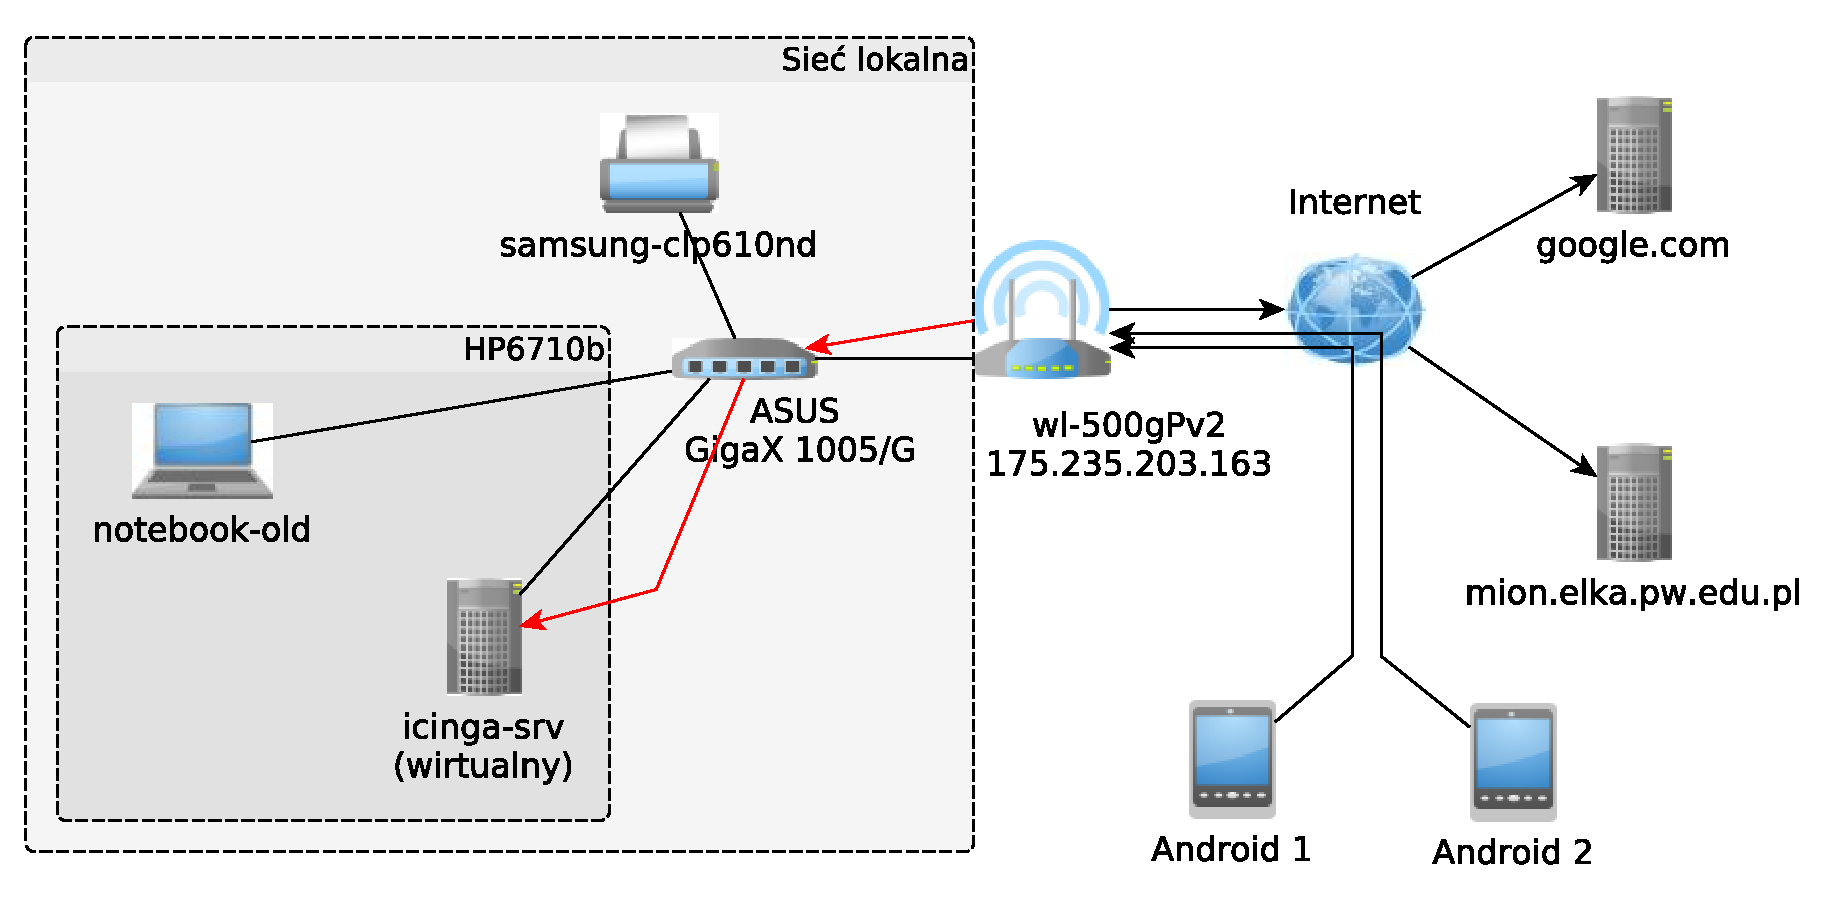
\includegraphics[width=1\textwidth]{img/schematSieci}
\end{figure}

\begin{table}
\centering
\caption{Objaśnienia nazw urządzeń wykorzystywanych w~infrastrukturze.}
\label{tab:devices}
\begin{tabular}{|p{4cm}||p{10cm}|}
  \hline
  Nazwa & Opis \\
  \hline \hline
  notebook-old & System zainstalowany natywnie na laptopie HP 6710b. \\
  \hline
  icinga-srv & System uruchomiony na maszynie wirtualnej na urządzeniu notebook-old. \\
  \hline
  samsung-clp610nd & Drukarka Samsung CLP-610ND znajdująca się w sieci lokalnej \\
  \hline
  \raggedright{wl-500gPv2 175.235.203.163} & \raggedright{Router ASUS WL-500GPv2 o zewnętrznym adresie IP 175.235.203.163}
  \tabularnewline
  \hline
  google.com & Serwer popularnej wyszukiwarki internetowej Google. \\
  \hline
  mion.elka.pw.edu.pl & Serwer mion zarządzany przez WEiTI PW. \\
  \hline
  Android 1 & Telefon Samsung Galaxy Note 3. \\
  \hline
  Android 2 & Telefon Samsung Galaxy S2 Plus. \\
  \hline
\end{tabular}
\end{table}

\section[Konfiguracja systemu monitorowania][Konfiguracja systemu
monitorowania]{Konfiguracja systemu monitorowania}

Monitorowana infrastruktura jest dość prosta i~mała. Pozwala to na
użycie jednego rdzenia monitorującego zarówno do monitorowania
infrastruktury statycznej, jak i~do przetwarzania danych pochodzących
od klientów mobilnych. W~celu zapewnienia konfiguracji zbliżonej do
warunków użytkowania systemu, wykonano konifgurację wraz z dodatkien
inGraph oraz baza danych dla systemu Icinga. Konfiguracja całego
systemu składa się z~następujących elementów:

\begin{itemize}
\item rdzeń monitorujący Icinga,
\item baza danych MySQL systemu Icinga,
\item dodatek inGraph,
\item baza danych MySQL dodatku inGraph,
\item interfejs icinga-web,
\item baza danych MySQL icinga-web\footnote{Ze względu na użycie
    nowego interfejsu konieczna jest dodatkowa baza danych, w~której
    przechowywane są dane warstwy prezentacji. Baza ta nie została
    wymieniona w~opisie, gdyż nie zawiera ona danych o stanie sieci,
    a~jedynie dane interfejsu graficznego.},
\item wykonany w~tej pracy dodatek NSCAv2,
\item aplikacja mobilna dla platformy Android, napisana przez Pana
  Kubika,
\item zestaw wtyczek.
\end{itemize}

Aby zapewnić możliwość łatwego przeniesienia wykonanej konfiguracji
testowej wszystkie elementy poza aplikacjom mobilną zostały utworzone
na systemie zainstalowanym na maszynie wirtualnej\footnote{Możliwa
  jest oczywiście separacja elementów zgodnie z~opisem zawartym w~
  \ref{chap:ProjektSystemu}. Wykonanie jej w~tym przypadku jest jednak
  nieuzasadnione i doprowadziłoby jedynie do licznych utrudnień
  w~przypadku przeniesienia na inne urządzenie.}. Schemat
rozmieszczenia oraz współpracy poszczególnych elementów został
przedstawiony na \ref{fig:deployment}. System monitorowania do
poprawnego funkcjonowania potrzebuje zarówno serwera bazy danych
MySQL, jak i~serwera http. W~wykorzystywanej wersji dystrybucji Ubuntu
wymagane pakiety zostały zainstalowane domyślnie podczas instalacji
systemu.

\begin{figure}[ht]
  \caption{Diagram rozmieszczenia i~współpracy elementów systemu
    monitorowania.}
 \label{fig:deployment}
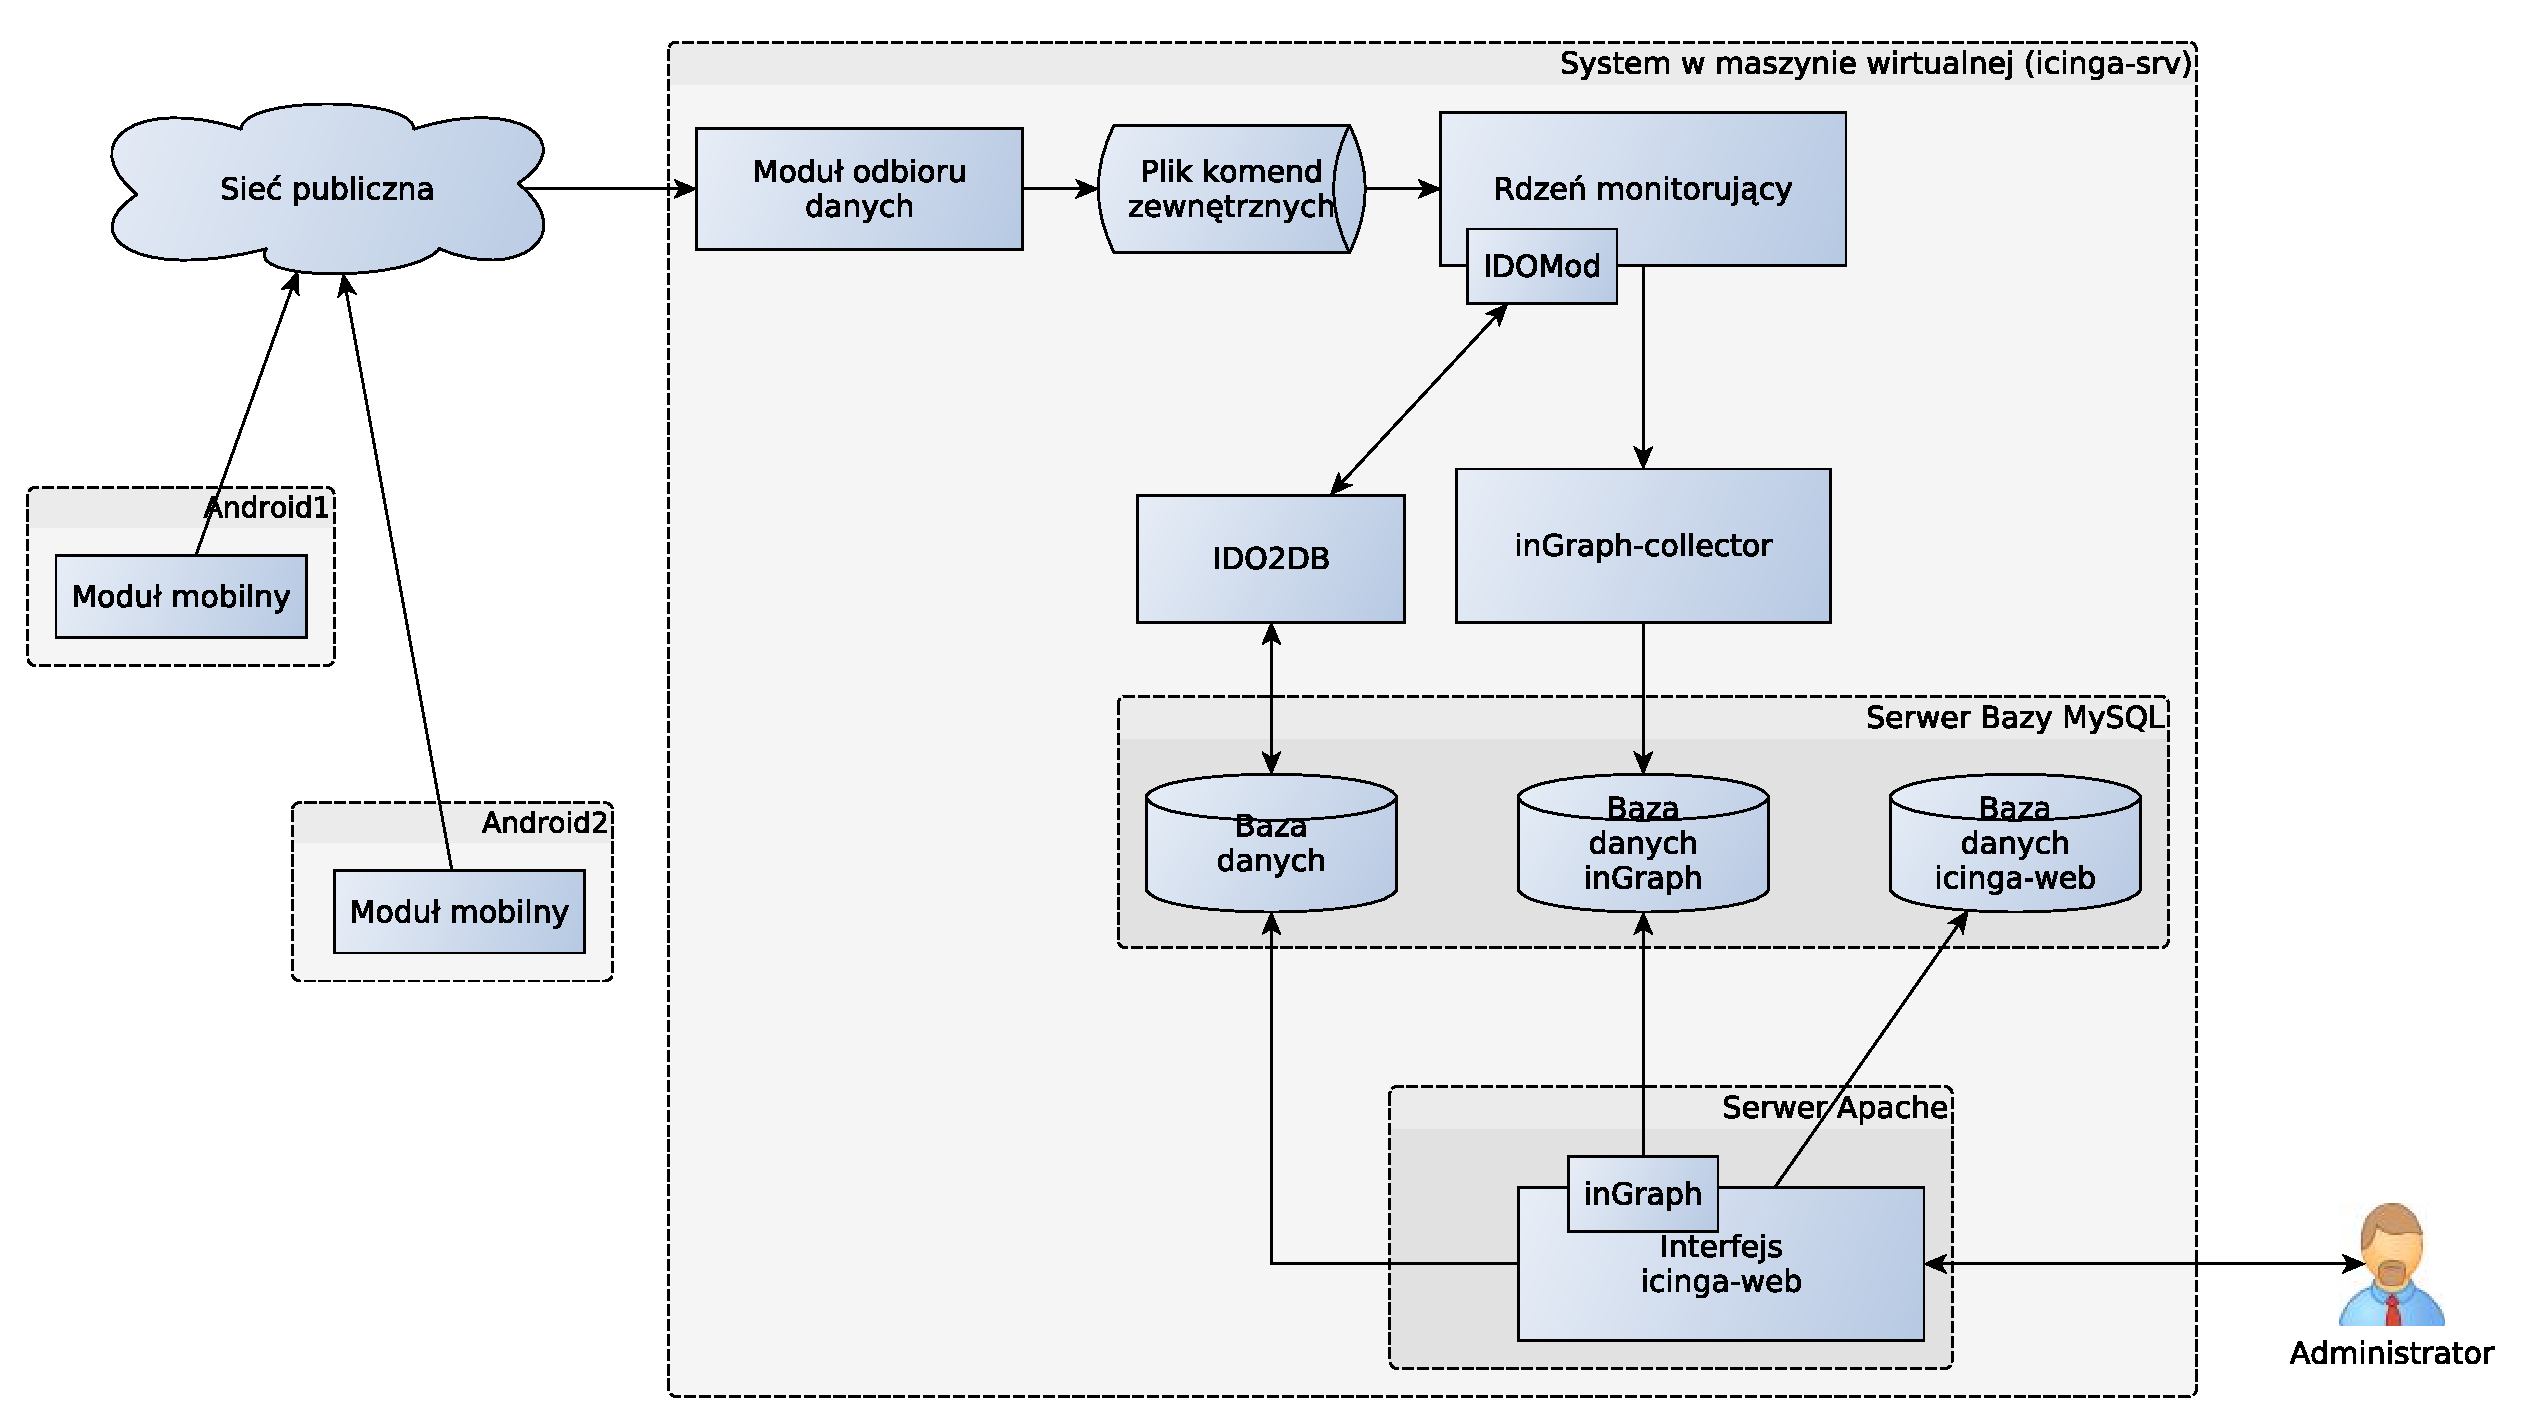
\includegraphics[width=1\textwidth]{img/deployment}
\end{figure}

Rdzeń systemu monitorowania został skonfigurowany tak, aby monitorować
w~sposób aktywny wszystkie usługi klientów statycznych. Do
monitorowania użyto zestawu standardowych wtyczek rozwijanych
pierwotnie dla systemu Nagios. Lista monitorowanych usług dla każdego
urządzenia została przedstawiona w~formie tabeli
\ref{tab:hostServiceStatic}. Niektóre z~monitorowanych wartości
wymagają użycia dodatkowego narzędzi - NRPE\footnote{ang. {\em Nagios
    Remote Plugin Executor} -- narzędzie do zdalnego uruchamiania
  wtyczek. Dokładny opis można znaleźć w~\cite{www:NRPE}.}. Jest to
narzędzie, które pozwala na uruchomienie wtyczki na zdalnej
maszynie. Jest on niezbędny do pomiaru parametrów wewnętrznych danego
urządzenia, takich jak zużycie procesora czy pamięci.

\begin{table}
\centering
\caption{Monitorowane usługi i parametry klientów statycznych}
\label{tab:hostServiceStatic}
\begin{tabular}{|p{2.5cm}|c|p{2cm}|p{2cm}|c|c|c|}
\hline
\raggedright{Wartość mierzona} & icinga-srv & \raggedright{notebook- -old} & \raggedright{samsung- -clp610nd} & wl-500gPv2 & google & mion \\
\hline
\raggedright{Liczba procesów} & \multicolumn{1}{|c|}{Tak} & \multicolumn{1}{|c|}{Tak}  &   &  &  &  \\
\hline

\raggedright{Użycie przestrzeni wymiany} & \multicolumn{1}{|c|}{Tak} &  &  &  &  &  \\
\hline

SSH & \multicolumn{1}{|c|}{Tak} & \multicolumn{1}{|c|}{Tak} &  &  &  & \multicolumn{1}{|c|}{Tak} \\
\hline

Użycie dysku & \multicolumn{1}{|c|}{Tak} &  &  &  &  &  \\
\hline

HTTP & \multicolumn{1}{|c|}{Tak} & \multicolumn{1}{|c|}{Tak} & \multicolumn{1}{|c|}{Tak} & \multicolumn{1}{|c|}{Tak} & \multicolumn{1}{|c|}{Tak} & \multicolumn{1}{|c|}{Tak} \\
\hline

\raggedright{Liczba zalogowanych użytkowników} & \multicolumn{1}{|c|}{Tak} & \multicolumn{1}{|c|}{Tak} &  &  &  &  \\
\hline

\raggedright{Bieżące obciążenie} & \multicolumn{1}{|c|}{Tak} & \multicolumn{1}{|c|}{Tak} &  &  &  &  \\
\hline

Ping & \multicolumn{1}{|c|}{Tak} & \multicolumn{1}{|c|}{Tak} & \multicolumn{1}{|c|}{Tak} & \multicolumn{1}{|c|}{Tak} & \multicolumn{1}{|c|}{Tak} & \multicolumn{1}{|c|}{Tak} \\
\hline

\raggedright{Liczba procesów} & \multicolumn{1}{|c|}{Tak} &  &  &  &  &  \\
\hline

IMAP z SSL &  &  &  &  &  & \multicolumn{1}{|c|}{Tak} \\
\hline

POP3 z SSL &  &  &  &  &  & \multicolumn{1}{|c|}{Tak} \\
\hline

SMTP &  &  &  &  &  & \multicolumn{1}{|c|}{Tak} \\
\hline

\raggedright{Liczba procesów zombie} &  & \multicolumn{1}{|c|}{Tak} &  &  &  &  \\
\hline
\end{tabular}
\end{table} 

W celu umożliwienia monitorowania klienta mobilnego konieczne było
również zdefiniowanie w~systemie Icinga urządzeń Android1 oraz
Android2, a~także odpowiednich usług. Udostępniona przez Pana Marcina
Kubika wersja aplikacji mobilnej posiada duży zbiór parametrów
urządzenia, które można monitorować. Spośród dostępnych parametrów
wybrano następujące:

\begin{itemize}
\item siła najmocniejszego sygnału Wi-Fi,
\item stan baterii,
\item liczba uruchomionych aplikacji,
\item obciążenie procesora.
\end{itemize}

Konieczna była również konfiguracja dodatku NSCAv2. Ponieważ telefony
posiadały różnych użytkowników, zostały utworzone dwa konta
klientów. Jako jedyną dopuszczalną metodę uwierzytelnienia wybrano
login oraz hasło. W~celu zapewnienia transportu danych konieczne było
również nadanie utworzonym użytkownikom uprawnień dotyczących urządzeń
i usług. W~celu umożliwienia przesłania danych od klienta konieczna
była konfiguracja dostawcy danych. Pierwszym jej etapem było
wygenerowanie pary kluczy RSA oraz umieszczenie klucza prywatnego
i~publicznego na serwerze, a~publicznego na urządzeniach
mobilnych. Konieczne było również podanie w~pliku konfiguracyjnym
dodatku NSCAv2 ścieżki do klucza prywatnego, a~także numeru portu na
którym powinien on czekać na przychodzące połączenia. Ponieważ plik
komend zewnętrznych w~wykonanej instalacji systemu Icinga znajduje się
w~standardowym miejscu, konieczna była jedynie bezparametrowa
deklaracja konsumenta danych. Ostatnim etapem konfiguracji było
zdefiniowanie ścieżki danych dla klientów, prowadzącej od dostawcy
danych do odbiorcy.

Przedstawiona na rys.~\ref{fig:schematSieci} topologia sieci wyraźnie
pokazuje, że istnieje w~sieci urządzenie, którego awaria może
spowodować utratę łączności z~wieloma urządzeniami. Elementem tym jest
router wl-500gpv2. Awaria tego urządzenia powoduje, że serwer icinga
traci możliwość wykonywania sprawdzeń zarówno tego urządzenia, jak
i~wszystkich urządzeń znajdujących się poza siecią lokalną. W~celu
ograniczenia liczby komunikatów otrzymywanych w~przypadku takiej
awarii konieczne było zdefiniowanie odpowiedniej struktury
sieci. Rysunek \ref{fig:logicznySchematSieci} przedstawia logiczną
strukturę połączeń. Została ona wygenerowane przez program Icinga na
podstawie plików konfiguracyjnych monitorowanych urządzeń. Łatwo
zauważyć, że jedyna ścieżka od systemu monitorującego do wszystkich
urządzeń spoza sieci lokalnej prowadzi przez router
wl-500gpv2. Odpowiada to oczywiście fizycznym zależnościom w~sieci
i~umożliwi precyzyjną diagnozę ewentualnej awarii.

\begin{figure}[ht]
  \caption{Logiczny schemat monitorowanej
    infrastruktury.}
  \label{fig:logicznySchematSieci}
  \centering
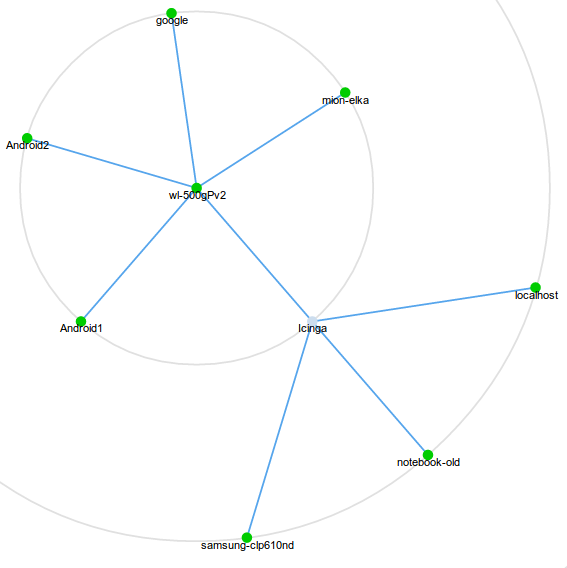
\includegraphics[width=0.8\textwidth]{img/logicznySchematSieci.png}
\end{figure}

\section[Klient statyczny][Rezultaty dla klientów statycznych]{Rezultaty dla klientów statycznych}

Monitorowanie infrastruktury statycznej zostało przeprowadzone
w~okresie trzech tygodni. Czas ten jest zdecydowanie wystarczający, aby
zgromadzić dane, będące wiarygodnym źródłem informacji o~sieci. Należy
zauważyć, że system monitorowania działał przez cały ten czas bez
żadnej awarii.

\subsection[Sieć lokalna][Sieć lokalna]{Sieć lokalna}

Testowanie monitorowania sieci lokalnej przebiegło zgodnie
z~oczekiwaniami. Zgromadzone dane wykazały stałą jakość usług
świadczonych w~sieci lokalnej. Ze względu na niski poziom
skomplikowania infrastruktury testowej, otrzymywane wartości czasu od
wysłania pakietu do jego powrotu były rzędu pojedynczych
milisekund. Dzięki wykorzystaniu dodatku inGraph możliwe było
przedstawienie zgromadzonych danych w~formie wykresów.

Przykładowy wykres czasu podróży pakietów oraz poziomu utraconych
podczas komunikacji pakietów dla router wl-500gPv2 przedstawiono na
rys.~\ref{fig:pingRoutera}. Na wykresie kolorem zielonym zostały
zaznaczone średnie czasy podróży dla zadanych przedziałów. Kolor szary
prezentuje natomiast wartości minimalne i~maksymalne dla bieżących
przedziałów agregacji. Kolor czerwony pokazuje udział utraconych
pakietów wobec wszystkich przesłanych.

\begin{figure}[ht]
  \caption{Wykres wartości czasu podróży pakietu oraz stopnia
    utraconych pakietów dla wl-500gPv2. Wykresy przedstawiają
    odpowiednio okres jednego dnia, tygodnia oraz miesiąca.}
  \label{fig:pingRoutera}
  \centering
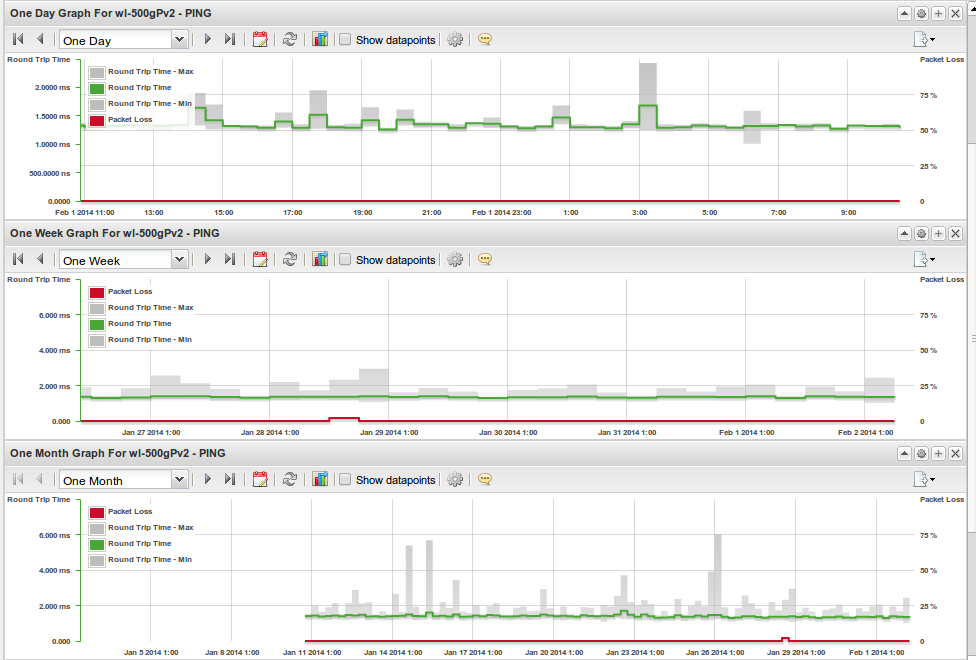
\includegraphics[width=1\textwidth]{img/pingRoutera.png}
\end{figure}

Przedstawiony wykres potwierdza prawidłowe wyniki przeprowadzonych
testów systemu. Średni czas podróży pakietu wynosi poniżej 2
ms. Uzyskane wartości maksymalne są rzędu 6 ms, co również jest
zjawiskiem normalnym w~sieciach komputerowych, ze względu na zmienne
obciążenie routera. Należy zauważyć, że na wykresie wystąpił chwilowy
wzrost stopnia utraconych pakietów w~okolicach 29 stycznia. Dodatek
inGraph pozwala administratorowi, po zauważeniu takiej sytuacji
wygenerować wykres dokładniejszych wartości we wskazanym
okresie. Funkcja szybkiego widoku, która pozwala na zaznaczenie
interesującego obszaru pozwoliła na łatwe przedstawienie dokładnych
danych z~okresu wystąpienia wzrostu mierzonej wartości. Wykres ten
został przedstawiony na \ref{fig:pingRouteraDokladny}. Na podstawie
tego wykresu można określić dokładny czas wystąpienia interesującego
zdarzenia. W~przypadku wystąpienia usterki może to zostać
wykorzystane do diagnozowania jej przyczyny poprzez badanie zdarzeń
tuż przed jej wystąpieniem.

\begin{figure}[ht]
  \caption{Wykres wartości czasu podróży pakietu oraz stopnia
    utraconych pakietów dla wl-500gPv2 w okresie, gdzie wystąpił wzrost stopnia utraconych pakietów.}
  \label{fig:pingRouteraDokladny}
  \centering
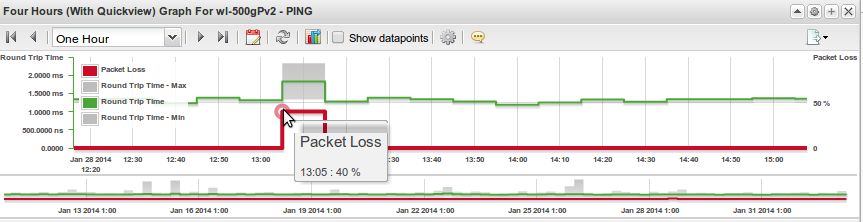
\includegraphics[width=1\textwidth]{img/pingiRouterDokladny.png}
\end{figure}

\subsection[Serwery zewnętrzne][Serwery zewnętrzne]{Serwery zewnętrzne}

Sieć lokalna jest wykorzystywana jedynie przez wąskie grono
użytkowników. Powoduje to niewielką zmienność monitorowanych w~niej
parametrów. Dzięki monitorowaniu serwerów zewnętrznych możliwe było
przetestowanie systemu w~dużo bardziej realistycznych warunkach.

Monitorowanie popularnego i~ogólnodostępnego serwera google.com
pozwoliło na przetestowanie systemu z~realnym systemem o~dużym
i~bardzo zmiennym obciążeniu. Rezultaty monitorowania serwisu zostały
przedstawione w~formie wykresu na rys.~\ref{fig:pingiGoogle}. Nawet
pobieżna analiza takiego wykresu pozwala zauważyć obecne w~nim
trendy. Na podstawie wykresu miesięcznego można zauważyć cykliczne
wzrosty wartości maksymalnej dla zadanych przedziałów
agregacji. Wykres ten pokazuje, iż występują one praktycznie
codziennie. Analiza wykresu tygodniowego pozwala dodatkowo na
określenie, że wspomniane skoki wartości maksymalnej występują
w~godzinach wieczornych. Ponadto łatwo zauważyć, że każdego dnia
w~godzinach popołudniowych i~wieczornych występuje znaczny wzrost
średniego czasu odpowiedzi serwera. Dzięki dynamicznemu charakterowi
wykresów programu inGraph możliwe jest dokonanie dokładnej analizy
widocznych na wykresie tendencji.

\begin{figure}[ht]
  \caption{Wykres wartości czasu podróży pakietu oraz stopnia
    utraconych pakietów dla google.com.  Wykresy przedstawiają
    odpowiednio okres jednego dnia, tygodnia oraz miesiąca.}
  \label{fig:pingiGoogle}
  \centering
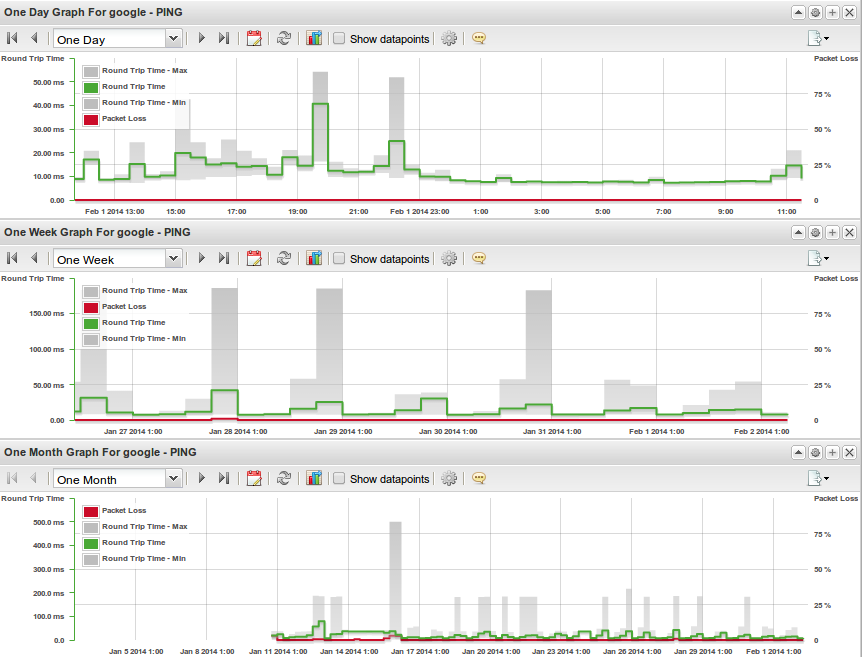
\includegraphics[width=1\textwidth]{img/pingiGoogle.png}
\end{figure}


Rysunki \ref{fig:google3001}, \ref{fig:google2801} oraz
\ref{fig:google2701} przedstawiają dokładniejsze dane z~przedziałów,
w~których notowano wzrosty czasu odpowiedzi. Analiza tych wykresów
pozwoliła na potwierdzenie tezy o~powtarzającej się tendencji. Łatwo
można zauważyć, że w~każdym z~pokazanych przedziałów notowany jest
stopniowy wzrost czasu odpowiedzi serwera od godziny 15. Godziny
wieczorne to na każdym z~wykresów zdecydowany wzrost czasu odpowiedzi,
a~także jego chwilowe piki. Od około godziny 12 w~nocy pojawia się
spadek czasu odpowiedzi serwera, który utrzymuje się na niskim
poziomie aż do godziny 15. Uzyskane rezultaty są zgodne
z~oczekiwanymi. Okres, w~którym czas odpowiedzi serwera znacząco
wzrasta, przypada na tak zwane internetowe godziny szczytu, czyli
okres pomiędzy godziną 19 i 21. Zjawisko to zostało opisane
w~\cite{www:RushHours}.


\begin{figure}[H]
  \caption{Wykres wartości czasu podróży pakietu oraz stopnia
    utraconych pakietów dla google.com dnia 30.01.2014.}
  \label{fig:google3001}
  \centering
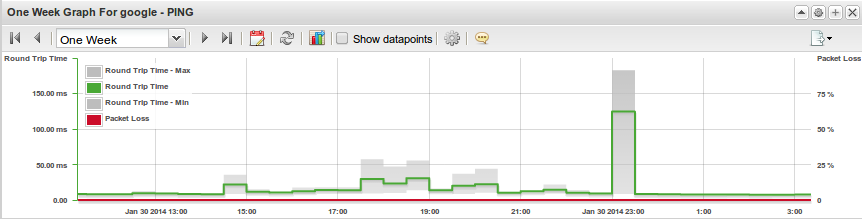
\includegraphics[width=1\textwidth]{img/google3001.png}
\end{figure}

\begin{figure}[H]
  \caption{Wykres wartości czasu podróży pakietu oraz stopnia
    utraconych pakietów dla google.com dnia 28.01.2014.}
  \label{fig:google2801}
  \centering
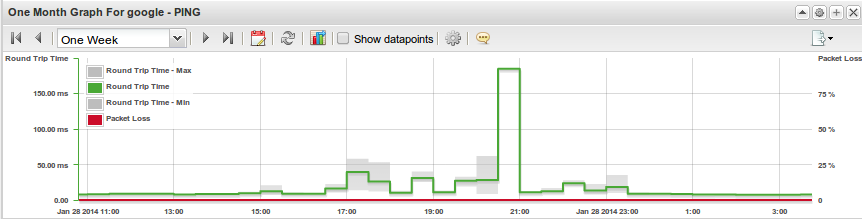
\includegraphics[width=1\textwidth]{img/google2801.png}
\end{figure}

\begin{figure}[H]
  \caption{Wykres wartości czasu podróży pakietu oraz stopnia
    utraconych pakietów dla google.com dnia 27.01.2014.}
  \label{fig:google2701}
  \centering
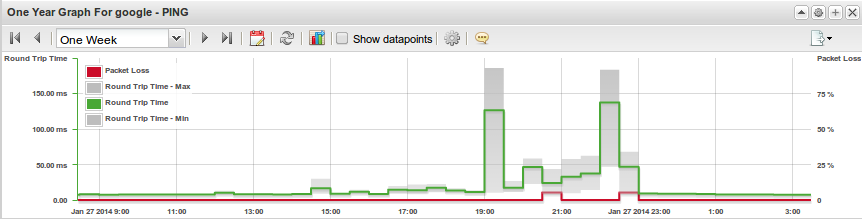
\includegraphics[width=1\textwidth]{img/google2701.png}
\end{figure}


\section[Klient mobilny][Rezultaty dla klientów mobilnych]{Rezultaty dla klientów mobilnych}

Monitorowanie klienta mobilnego odbyło się w~czasie jednego
tygodnia. Okres ten jest już znacznej długości, a~codzienne używanie
monitorowanych telefonów pozwoliło na wiarygodną symulację prawdziwych
warunków funkcjonowania systemu.

Przeprowadzone testy pozwoliły wykazać poprawność działania wszystkich
pożądanych mechanizmów. Pierwszym z~przetestowanych mechanizmów było
zapewnienie monitorowania stanu bieżącego usług i~parametrów urządzeń
mobilnych w~sposób analogiczny jak urządzeń statycznych. System
działał zgodnie z~oczekiwaniami, dzięki czemu wszystkie ostrzeżenia
były odpowiednio generowane. Przykładem takiego komunikatu jest
powiadomienie administratora o~stanie krytycznym baterii, które
zostało przedstawione na~\ref{fig:criticalBat}.

\begin{figure}[ht]
  \caption{Pulpit stanów poszczególnych usług i~parametrów klientów
    mobilnych.}
  \label{fig:criticalBat}
  \centering
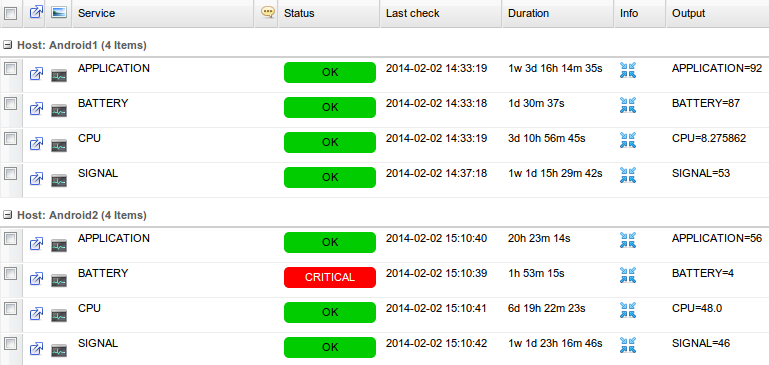
\includegraphics[width=1\textwidth]{img/criticalBat.png}
\end{figure}

Kolejną istotną funkcjonalnością, która była w~tym czasie testowana,
jest gromadzenie danych historycznych pochodzących od klienta
mobilnego. Mechanizm gromadzenia tych danych i~ich analizy działały
podczas testów bez zarzutu. Pozwoliło to na wykonanie wykresów
mierzonych wartości. Przykładowy wykres stanu baterii dla obu urządzeń
wygenerowany na podstawie danych zebranych w~czasie testów zawarto na
\ref{fig:baterie}.
 
\begin{figure}[ht]
  \caption{Wykres stanu baterii urządzeń mobilnych w okresie
    testowania systemu. Pierwszy wykres (u góry) pokazuje stan baterii
    urządzenia Android 1, drugi (na dole) --- urządzenia Android2.}
  \label{fig:baterie}
  \centering
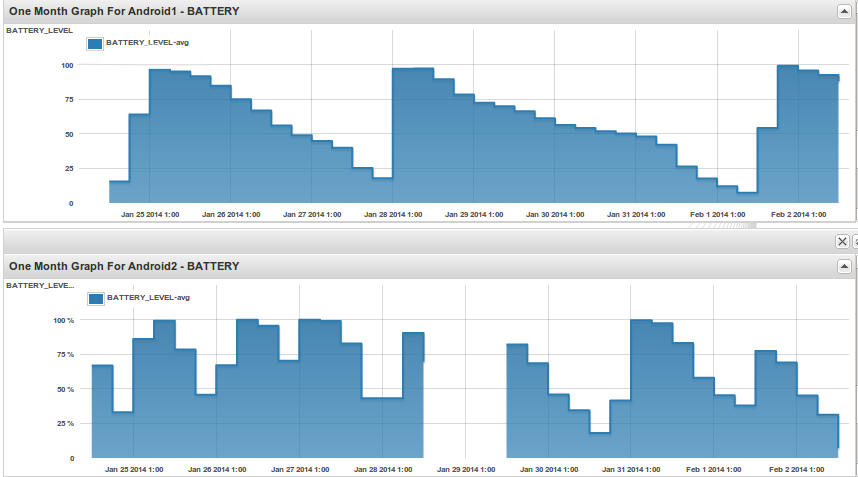
\includegraphics[width=1\textwidth]{img/battery.png}
\end{figure}

Widoczna na jednym z~wykresów przerwa wynika z~braku danych w~tym
okresie. Ze względu na równolegle powstawanie pracy inżynierskiej Pana
Marcina Kubika, który jest właścicielem tego urządzenia, konieczne było
wyłączenie go na jeden dzień z~testów systemu. Na przedstawionych
wykresach można wyróżnić dwie fazy. Pierwsza z~nich to rozładowywanie
baterii. Okres ten można rozpoznać po zmniejszającym się pomiędzy
kolejnymi pomiarami stanem baterii. Okres ładowania widoczny jest na
wykresie jako czas gwałtownego wzrostu stanu baterii. Na podstawie
wykresu można oszacować, iż bateria urządzenia Android1 była ładowana
3 razy, natomiast urządzenia Android2 co najmniej 6 razy. Wskazuje to
na znaczne zużycie baterii w~drugim urządzeniu lub jego bardzo
intensywne użytkowanie.

Ponadto na podstawie przedstawionego wykresu można wnioskować o~stylu
użytkowania obu telefonów. Urządzenie Android1 ładowane jest do bardzo
wysokiego poziomu baterii, a~następnie użytkownik oczekuje z jego
ładowaniem aż poziom baterii spadnie poniżej 20\%. Użytkownik
urządzenia Android2 natomiast bardzo często wykonuje ładowanie swojego
telefonu nawet przy stanie powyżej 50\%. W~zależności od typu baterii
znajdującej się w urządzeniu, takie działanie może skracać jej
żywotność.

Możliwość analizy sposobu użytkowania danego urządzenia może być dla
Administratora bardzo pomocne. Może to zostać wykorzystane np. do
lepszego zarządzania rozdziałem urządzeń mobilnych w firmie. Ponadto
jeśli monitorowane urządzenia mobilne posiadają znaczną wartość, to
śledzenie stylu ich użytkowania również jest niezwykle istotne, aby
zapewnić ich długą żywotność.

W~trakcie testów monitorowano również siłę sygnały Wi-Fi. Rezultaty
pomiarów przedstawiono na rysunku \ref{fig:signals}. Ponownie na
wykresie dla urządzenia drugiego widoczna jest przerwa wynikająca
z~chwilowego wyłączenia urządzenia z~testów. Na podstawie tych
wykresów łatwo można zauważyć, że urządzenie Android1 posiada znacznie
częstszy i~znacznie lepszy dostęp do sieci Wi-Fi niż urządzenie
Android2. Można wręcz zauważyć, iż urządzenie Android2 jest typowym
klientem mobilnym, który dostęp do sieci uzyskuje bardzo
sporadycznie. Słaba siła sygnału sieci Wi-Fi powoduje oczywiście
zwiększone zużycie baterii, co jest widoczne na wykresie
\ref{fig:baterie}.

\begin{figure}[ht]
  \caption{Wykres sygnału sieci Wi-Fi w okresie testowania
    systemu. Pierwszy wykres (u góry) pokazuje sygnał dla urządzenia
    Android1, drugi (na dole) --- urządzenia Android2.}
  \label{fig:signals}
  \centering
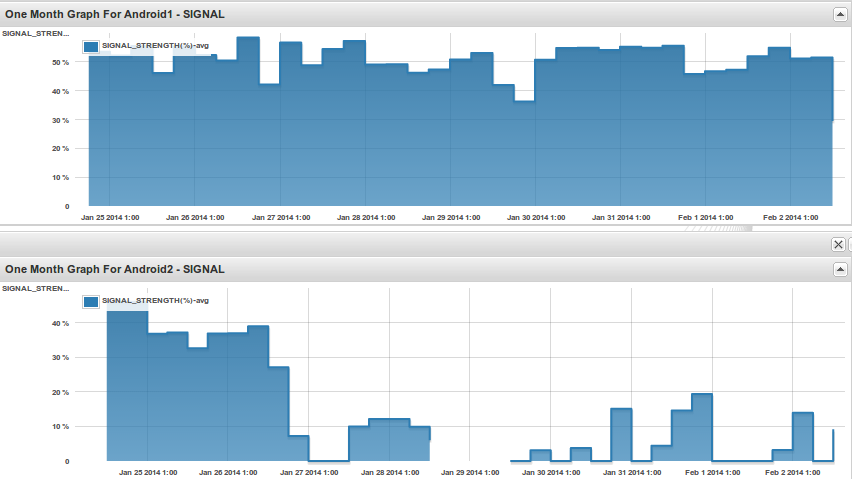
\includegraphics[width=1\textwidth]{img/wifi.png}
\end{figure}

W~zastosowaniu produkcyjnym analiza takich danych jak dostępność sieci
Wi-Fi w~miejscu codziennego użytku urządzenia mobilnego jest niezwykle
istotna. Firmy wydają bardzo duże pieniądze na zakup pakietów danych
u~operatorów sieci komórkowych w~celu zapewnienia swoim pracownikom
łączności z~Internetem. Na podstawie analizy siły sygnału sieci dla
każdego klienta można w~dużo lepszy sposób zarządzać limitami danych
otrzymanymi od operatora. Jeśli część klientów mobilnych przebywa
przez większość czasu w~zasięgu sieci Wi-Fi, to być może należy
ograniczyć przyznane dla nich limity na rzecz zwiększenia
przepustowości sieci bezprzewodowej. Ponadto dane o~sile sygnałów
pochodzące z~wielu urządzeń pozwalają na badanie wpływu rozmieszczenia
punktów dostępowych na zasięg sieci w~siedzibie firmy.

\chapter{Podsumowanie}
\label{chap:Podsumowanie}

W~ramach tej pracy wykonano projekt oraz implementację rozszerzenia
systemu Icinga na potrzeby monitorowania klientów mobilnych.
Zaprojektowany system został oparty na istniejących już elementach,
których wykorzystanie pozwoliło na uzyskanie bardzo rozbudowanej
funkcjonalności stosunkowo ograniczając nakład niezbędnej pracy.

Przed wykonaniem projektu przeprowadzono analizę dostępnych na rynku
systemów monitorujących. Zidentyfikowane problemy monitorowania
klientów statycznych oraz szczególny charakter klientów mobilnych
wskazały na potrzebę opracowania nowych rozwiązań.  W~ramach analizy
przedstawiono podstawowe możliwości otwartoźódłowych systemów {\em
  Cacti}, {\em Nagios} oraz {\em Icinga}. Porównanie tych systemów
wykazało, że najlepszym systemem do rozbudowy w~ramach tej pracy
będzie system {\em Icinga}.  Przedstawiono wymagania, jakie powinny
zostać spełnione przez projektowany system monitorujący, aby
umożliwiał on efektywne monitorowanie systemów mobilnych.

Kolejnym etapem przygotowania projektu była dokładna analiza
możliwości systemu {\em Icinga} w~kontekście zdefiniowanych
wymagań. W~ramach tej analizy przedstawiono ogólną architekturę
systemu oraz zestaw dopuszczalnych jego konfiguracji. Dokonano również
analizy dostępnych dodatków w~kontekście ich funkcjonalności i~jakości
ich wykonania. Ze względu na brak gotowych rozwiązań pozwalających na
monitorowanie klienta mobilnego zdefiniowano własny bezpieczny
protokół komunikacyjny. Zapewnia on bezpieczny transport danych
pomiędzy urządzeniem mobilnym a~serwerem monitorującym. Konieczne było
również wykonanie odpowiedniego dodatku do systemu {\em Icinga}, który
umożliwiłby odbiór danych od klientów mobilnych i~przekazanie ich do
miejsc zgodnych z~polityką całego systemu
monitorującego. 

Na podstawie projektu wykonano w~języku C++ implementację dodatku
NSCAv2. W~trakcie prac wykorzystany został szkielet aplikacji {\em
  Qt}, a~także biblioteka {\em boost}. Wszystkie algorytmy
kryptograficzne wymagane do implementacji protokółu komunikacyjnego
zostały zaimplementowane z~użyciem biblioteki {\em Crypto++}.

Końcowym etapem tej pracy było wdrożenie przykładowej konfiguracji
systemu {\em Icinga} zgodnie z~przedstawionym projektem i~z~użyciem
zaimplementowanego dodatku. Środowisko testowe zostało wykonane
w~domowej sieci lokalnej, jednak monitorowaniu podlegały również
publiczne serwery {\em google.com} oraz {\em
  mion.elka.pw.edu.pl}. Dzięki życzliwości Pana Marcina Kubika, który
wykonał implementację aplikacji mobilnej przeznaczonej na platformę
Android, możliwe było włączenie do środowiska testowego również dwóch
urządzeń pracujących pod kontrolą tego systemu.

Instancja systemu {\em Icinga} funkcjonowała nieprzerwanie przez trzy
tygodnie, co zapewniło zgromadzenie reprezentatywnego zbioru
danych. Wykorzystanie zewnętrznej infrastruktury zarówno do
monitorowania publicznych serwerów, jak i~przekazywania danych od
klientów mobilnych pozwoliło na symulację rzeczywistych warunków pracy
takiego systemu.

Zebrane dane potwierdziły przydatność zaprojektowanego systemu. Na ich
podstawie wskazano istotne trendy występujące w~sieciach
publicznych. Przeprowadzone testy wykazały również przydatność systemu
monitorującego klienta mobilnego. Dane zebrane w~trakcie monitorowania
takiego urządzenia mogą posłużyć dużym firmom do redukcji kosztów
utrzymania tych urządzeń i~optymalizacji posiadanej infrastruktury
sieciowej.

Jest bardzo wiele możliwych dróg rozwoju wykonanego projektu. Pierwszą
z~nich jest wykonanie narzędzia umożliwiającego w~łatwy i~intuicyjny
sposób zarządzanie konfiguracją systemu monitorującego i~jego
dodatków. Drugą, zdecydowanie ważniejszą i~dającą większe możliwości
rozwoju systemu, jest wykonanie systemu eksperckiego. System taki
mógłby na podstawie zgromadzonych danych historycznych (awariach,
parametrach wydajnościowych, zdarzeniach itp.) wykrywać z
wyprzedzeniem i~ostrzegać o~możliwości zaistnienia określonych
sytuacji. Pozwoliłoby to administratorowi podejmować odpowiednie kroki
zaradcze.


\appendix

% tutaj załączniki

%\chapter*{Bibliografia}
\nocite{*}
\bibliographystyle{plplain}
%\bibliographystylebk{plplain}
%\bibliographystylest{plplain}
%\bibliographystyledoc{plplain}
% \bibliographystyleweb{plplain}
%\bibliographybk{BIB/books}
%\bibliographyst{BIB/books}
%\bibliographydoc{BIB/books}
% \bibliographyweb{BIB/books}

% \bibliography{bib/verificard,bib/jml,bib/daikon}
%\bibliography{bib/daikon,bib/statistics,bib/other}
\bibliography{bib/www}
\end{document}

% ex: set tabstop=4 shiftwidth=4 softtabstop=4 noexpandtab fileformat=unix filetype=tex spelllang=pl,en spell:

